% +++
% latex="texfot lualatex-dev"
% +++
\documentclass[aspectratio=149,9pt,fleqn]{beamer}
\usetheme[numbering=fraction,block=fill]{metropolis}
\usefonttheme{professionalfonts}

\usepackage{luatexja,luatexja-adjust}
\usepackage[no-math,match,deluxe]{luatexja-fontspec}

\hypersetup{unicode,colorlinks}
\hypersetup{linkcolor=blue,urlcolor=teal,citecolor=olive}
% \hypersetup{linkcolor=black,urlcolor=black,citecolor=black}

\usepackage{pxrubrica}
\usepackage{autobreak}
\usepackage{tikz,pgfplots,tcolorbox}
\usetikzlibrary{calc}
\pgfplotsset{compat=1.16}

\usepackage[version=4,arrows=pgf]{mhchem}
\mhchemoptions{textfontcommand=\sffamily,mathfontcommand=\mathsf}
\newcommand*\cec[1]{\cesplit{{\,\ }{\0}}{#1}}

\usepackage{tabularray}
\SetTblrDefault{rowsep=0pt}

\usepackage[loadonly,]{enumitem}
\newlist{desc}{description}{5}
\setlist[desc]{labelindent=2\zw,labelsep*=1\zw,labelwidth=3\zw}
\newlist{enu}{enumerate}{5}
\setlist[enu]{label*=\arabic*.}

\ltjsetparameter{jacharrange={-2,-3,-8}}
\usepackage[no-math,match,deluxe,fontspec]{luatexja-preset}

% \usepackage[osf]{newpxtext}\usepackage{classico}
\usepackage[nowidering]{yhmath}
\usepackage{newpxmath,amsmath,mathtools,amssymb,mleftright}
\usepackage[T1]{fontenc}
\usepackage[notrig,italicdiff]{physics}
\mleftright

\usepackage[scr=boondoxo,frak=pxtx,bb=mth]{mathalfa}
\DeclareMathAlphabet{\mathnormal}{T1}{pplx}{m}{it}
\DeclareMathAlphabet{\mathrm}{T1}{pplx}{m}{n}
\DeclareMathAlphabet{\mathit}{T1}{pplx}{m}{it}
\DeclareMathAlphabet{\mathtt}{T1}{lmtt}{m}{n}
\DeclareMathAlphabet{\mathsf}{T1}{kurier}{m}{n}
\DeclareMathAlphabet{\mathbsf}{T1}{kurier}{b}{n}
\DeclareMathAlphabet{\mathbold}{T1}{pplx}{b}{it}
\DeclareMathAlphabet{\mathbf}{T1}{pplx}{b}{n}
\DeclareMathAlphabet{\mathscr}{U}{BOONDOX-calo}{m}{n}
\DeclareMathAlphabet{\mathbscr}{U}{BOONDOX-calo}{b}{n}
%\DeclareMathAlphabet{\mathcal}{OT1}{eusm10}{m}{n}
%\DeclareMathAlphabet{\mathbcal}{OT1}{eusm10}{b}{n}
\DeclareMathAlphabet{\mathfrak}{OT1}{tx-frak}{m}{n}
\DeclareMathAlphabet{\mathbfrak}{OT1}{tx-frak}{b}{n}
\DeclareMathAlphabet{\mathbb}{U}{dsss}{m}{n}
\DeclareSymbolFont{operators}{T1}{uop}{m}{n}

\DeclareSymbolFont{numbers}{T1}{pplx}{m}{n}
\DeclareMathSymbol{0}\mathalpha{numbers}{`0}
\DeclareMathSymbol{1}\mathalpha{numbers}{`1}
\DeclareMathSymbol{2}\mathalpha{numbers}{`2}
\DeclareMathSymbol{3}\mathalpha{numbers}{`3}
\DeclareMathSymbol{4}\mathalpha{numbers}{`4}
\DeclareMathSymbol{5}\mathalpha{numbers}{`5}
\DeclareMathSymbol{6}\mathalpha{numbers}{`6}
\DeclareMathSymbol{7}\mathalpha{numbers}{`7}
\DeclareMathSymbol{8}\mathalpha{numbers}{`8}
\DeclareMathSymbol{9}\mathalpha{numbers}{`9}

\DeclareFontFamily{U}{mathastro}{}
\DeclareFontShape{U}{mathastro}{m}{n}{<->mathastrotest10}{}
\DeclareSymbolFont{astro}{U}{mathastro}{m}{n}
\DeclareMathSymbol\Sun\mathord{astro}{'300}
\DeclareMathSymbol\Mercury\mathord{astro}{'301}
\DeclareMathSymbol\Venus\mathord{astro}{'302}
\DeclareMathSymbol\Earth\mathord{astro}{'303}
\DeclareMathSymbol\Mars\mathord{astro}{'304}
\DeclareMathSymbol\Jupiter\mathord{astro}{'305}
\DeclareMathSymbol\Saturn\mathord{astro}{'306}
\DeclareMathSymbol\Uranus\mathord{astro}{'307}
\DeclareMathSymbol\Neptune\mathord{astro}{'310}
\DeclareMathSymbol\Pluto\mathord{astro}{'311}
\DeclareMathSymbol\varEarth\mathord{astro}{'312}
\DeclareMathSymbol\Moon\mathord{astro}{'313}
\DeclareMathSymbol\leftmoon\mathord{astro}{'313}
\DeclareMathSymbol\rightmoon\mathord{astro}{'314}
\DeclareMathSymbol\fullmoon\mathord{astro}{'315}
\DeclareMathSymbol\newmoon\mathord{astro}{'316}
\DeclareMathSymbol\newmoon\mathord{astro}{'316}

\setmainfont[
	Ligatures=TeX,
	Scale=0.98,
	BoldFont=FOT-RodinNTLGPro-B,
	ItalicFont=FOT-RodinNTLGPro-B,
]{Palatino}
\setsansfont[
	Ligatures=TeX,
	Scale=0.98,
	BoldFont=FOT-RodinNTLGPro-B,
	BoldItalicFont=FOT-RodinNTLGPro-B,
	%ItalicFont=FOT-RodinNTLGPro-B,
]{Palatino}
\setmainjfont[
	Ligatures=TeX,
	JFM=jlreq,
	BoldFont=FOT-RodinNTLGPro-B,
	ItalicFont=FOT-RodinNTLGPro-B,
]{FOT-ModeMinBLargePro-M}
\setsansjfont[
	Ligatures=TeX,
	JFM=jlreq,
	BoldFont=FOT-RodinNTLGPro-B,
	ItalicFont=FOT-RodinNTLGPro-B,
]{FOT-ModeMinBLargePro-M}
\setmonofont[
	Ligatures=TeXReset,
]{HackGen}
\setmonojfont[
	Ligatures=TeXReset,
]{HackGen}

\allowdisplaybreaks[4]
\ltjenableadjust[lineend=extended,priority=true,profile=true,linestep=false]

%%%%%%%%%%%%自作マクロ
\newcommand{\hmvec}{\mathbold}
\newcommand{\hmeqdef}{\stackrel{\mathrm{def}}{=}}
\newcommand{\hmeqq}{\stackrel{\mathrm{?}}{=}}
\newcommand{\centeralign}[1]{\rule{0pt}{0pt}\hfill#1\hfill\rule{0pt}{0pt}}
\NewDocumentCommand\hmu{s m}{\IfBooleanF{#1}{\,}\ifmmode\mathrm{#2}\else\(\mathrm{#2}\)\fi}
\newcommand{\hmemph}[1]{\textbf{#1}}
\newcommand{\hme}[1]{\times10^{#1}}
\newcommand{\hmfnc}[1]{\(\mathrm{#1}\)}
\newcommand{\hmfconv}{F_\mathrm{conv}}
\NewDocumentCommand\etal{s}{\textit{et al.}\IfBooleanF{#1}{\ }}

\institute{北海道大学大学院理学院 地球流体力学研究室 M2}
\author{人見祥磨}
\title{水惑星における南北熱輸送の太陽定数への依存性}

\begin{document}

\maketitle

\begin{frame}
	\frametitle{背景}
	\begin{itemize}
		\item 系外惑星に生命が存在するためには、惑星表面に液体の水があることが
			重要だと考えられる (Kopparapu \etal*, 2013)
		\item 惑星表面に液体の水が存在しうる領域は、ハビタブルゾーン (HZ)と呼ばれる
		\item HZ より内側では、水が蒸発しきってしまうほど太陽定数が大きいと考えられる
		\item ここでは太陽定数を増やした時に気候がどう変化するか着目する
	\end{itemize}
	\begin{figure}
		\centering\scriptsize
		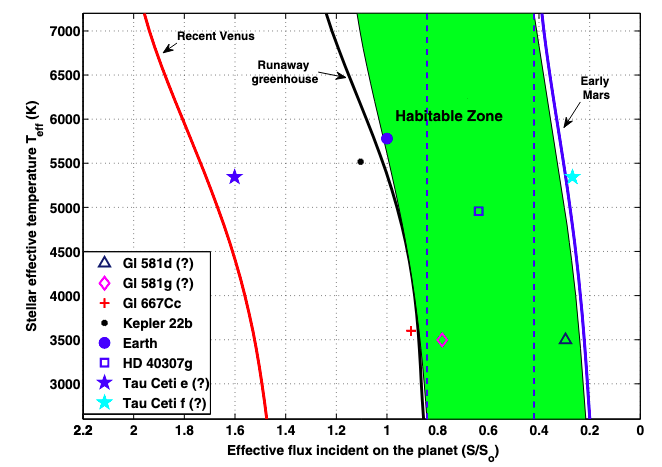
\includegraphics[width=.5\textwidth]{kopparapu8.png}\\
		様々な中心星の有効温度ごとに、雲がない場合の HZ を示したもの。
		(Kopparapu \etal*, 2013; Fig.\ 8)
	\end{figure}
\end{frame}

\begin{frame}
	\frametitle{暴走温室状態}
	\begin{itemize}
		\item HZ の内側境界を決定する重要な概念として、暴走温室状態がある
			\begin{itemize}
				\item 灰色 1 次元モデルでは惑星大気が射出できる放射に
					上限が存在する(放射上限)
				\item 放射上限を超えて恒星放射の入射がある状態が暴走温室状態
					である (Nakajima \etal 1992)
				\item 灰色 3 次元モデルでも放射上限は現れる (IshiwatAri \etal 2002)
			\end{itemize}
		\item 非灰色の 3 次元モデルでは暴走温室に関する議論は学会発表程度しかなかった
	\end{itemize}
	\begin{columns}[b,onlytextwidth]
		\begin{column}{.45\textwidth}
				\centering\scriptsize
				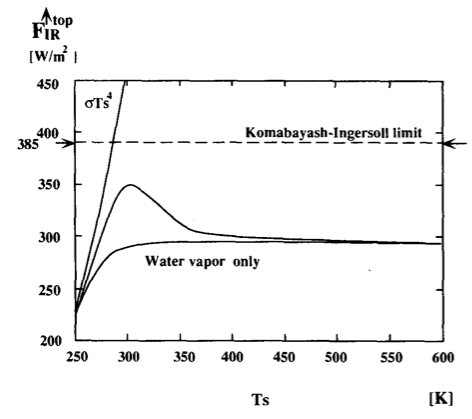
\includegraphics[width=.8\textwidth]{nf4.png}\\
				灰色 1 次元放射対流平衡モデルでの\\
				地表面温度と OLR の関係\\
				(Nakajima \etal*, 1992; Fig.\ 4)
		\end{column}
		\begin{column}{.45\textwidth}
			\begin{figure}
				\centering\scriptsize
				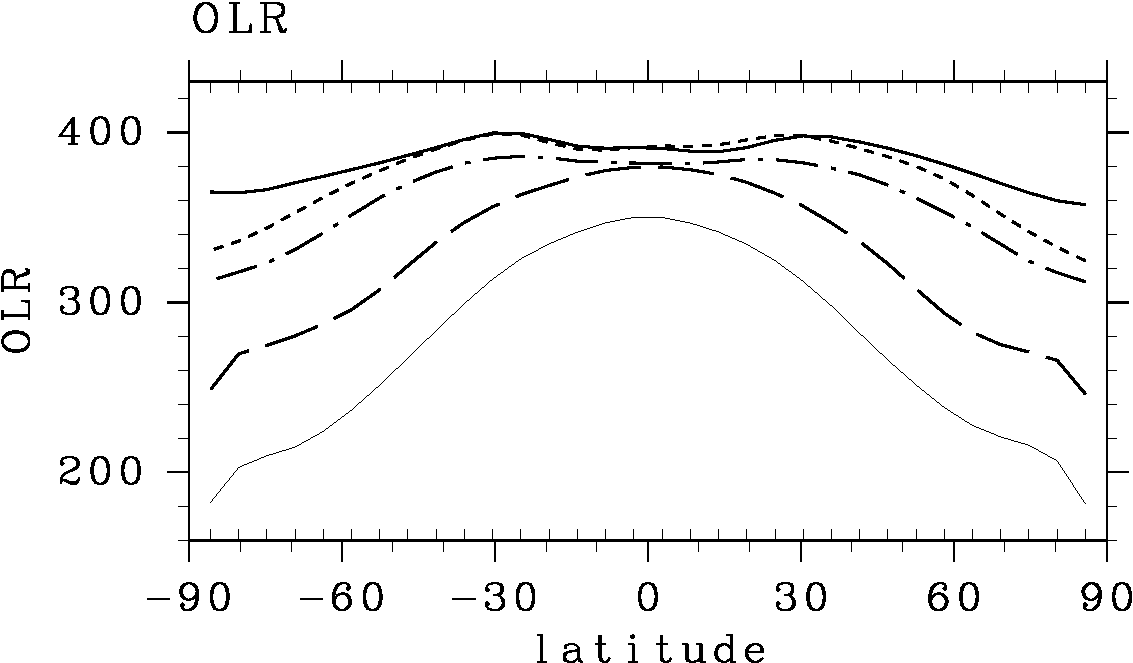
\includegraphics[width=.8\textwidth]{i20024a.pdf}\\
				灰色 3 次元モデルでの\\
				太陽定数と OLR の関係\\
				(\(S=1570, 1550, 1500, 1380, 1200\hmu{W/m^2}\))\\
				(Ishiwatari \etal*, 2002; Fig.\ 4a)
			\end{figure}
		\end{column}
	\end{columns}
\end{frame}


\begin{frame}
	\frametitle{研究目的}
	\begin{itemize}
		\item 非灰色の 3 次元モデルで太陽定数を変えて計算する
		\item 南北熱輸送に関して考察する
	\end{itemize}
\end{frame}

\begin{frame}
	\frametitle{モデル}
	\begin{columns}[T,onlytextwidth]
		\begin{column}{.45\textwidth}
			\begin{itemize}
				\item 利用したモデル
					\begin{itemize}
						\item DCPAM5
					\end{itemize}
				\item 基礎方程式
					\begin{itemize}
						\item 以下の 3 次元球殻上プリミティヴ方程式
					\end{itemize}
			\end{itemize}
		\end{column}
		\begin{column}{.45\textwidth}
		\end{column}
	\end{columns}
	\tiny
	\begin{gather*}
		\pdv{\pi}{t}+\hmvec{v}_H\cdot\nabla_\sigma\pi=-D-\pdv{\dot \sigma}{\sigma}\tag{連続の式}\\
		\pdv{\Phi}{\sigma}=-\frac{RT_v}{\sigma}\tag{静水圧の式}\\
		\pdv{\zeta}{t}=\frac{1}{a}\qty(\frac{1}{1-\mu^2}\pdv{V_A}{\lambda}-\pdv{U_A}{\mu})+\mathcal{D}[\zeta],\qquad
		\pdv{D}{t}=\frac{1}{a}\qty(\frac{1}{1-\mu^2}\pdv{U_A}{\lambda})
			-\nabla^2_\sigma(\Phi+R\bar T\pi+KE)+\mathcal{D}[D]\tag{運動方程式}\\
		\pdv{T}{t}=-\frac{1}{a}\qty(\frac{1}{1-\mu^2}\pdv{UT'}{\lambda}+\pdv{VT'}{\mu})+T'D-\dot\sigma\pdv{T}{\sigma}
			+\kappa T_v\qty(\pdv{\pi}{t}+\hmvec{v}_H\cdot\nabla_\sigma\pi+\frac{\dot\sigma}{\sigma})
			+\frac{Q}{C_p}+\mathcal{D}[T]+\mathcal{D}'[\hmvec{v}]\tag{熱力学の式}\\
		\pdv{q}{t}=-\frac{1}{a}\qty(\frac{1}{1-\mu^2}\pdv{U_q}{\lambda}+\pdv{V_q}{\mu})
			+qD-\dot\sigma\pdv{q}{\sigma}+S_q+\mathcal{D}[q]\tag{水蒸気の式}\\
	\end{gather*}
	\(\varphi,\lambda\): 緯度経度; \(\sigma:=p/p_s\): \(\sigma\) 座標高度; \(t\): 時間;
	\(\pi:=\ln[p_s]\); \(T\): 気温; \(q\): 比湿; \(a\): 惑星半径;\\
	\(\zeta:=(1/a)((1/(1-\mu^2))(\pdv*{V}{\lambda})-\pdv*{U}{\mu})\): 渦度;
	\(\zeta:=(1/a)((1/(1-\mu^2))(\pdv*{U}{\lambda})+\pdv*{V}{\mu})\): 発散;\\
	\(u,v\): 東西・南北風速; \((U,V):=(u\cos\varphi,v\cos\varphi)\);
	\(\mathcal{D}\): 水平拡散; \(\mathcal{D}'[\hmvec{v}]\): 摩擦熱;
\end{frame}

\begin{frame}
	\frametitle{実験設定}
	\begin{itemize}
		\item 水惑星
		\item 解像度 T42L26
		\item 太陽定数 \(S\) と積分時間
			\begin{center}
				\begin{tblr}{colspec={lrrrrr},hlines}
					\(S\hmu{[W/m^2]}\)&\(1366\)&\(1500\)&\(1600\)&\(1800\)&\(2000\)\\
					積分時間(年)&40&3&10&10&20\\
				\end{tblr}
			\end{center}
	\end{itemize}
\end{frame}

\begin{frame}
	\frametitle{結果 (OLRA の時間推移)}
	\begin{columns}[T]
		\begin{column}{.3\textwidth}
			\centering
			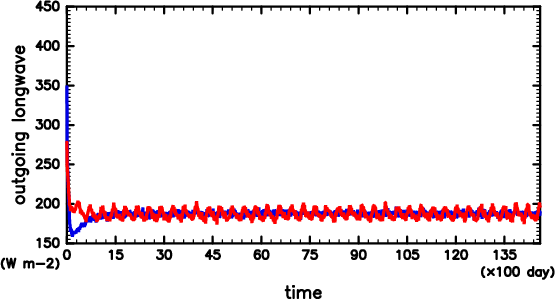
\includegraphics[width=\textwidth]{S1366/S1300_OLRA-OSRA_horimean_time0.0-14600.0-crop.png}
			\(S=1366\hmu{W/m^2}\)\\
			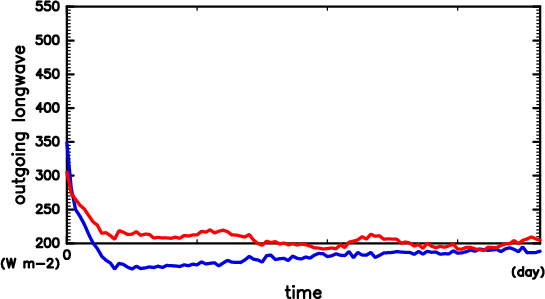
\includegraphics[width=\textwidth]{S1500/S1500_OLRA-OSRA_horimean_time0.0-1095.0-crop.png}
			\(S=1500\hmu{W/m^2}\)
		\end{column}
		\begin{column}{.3\textwidth}
			\centering
			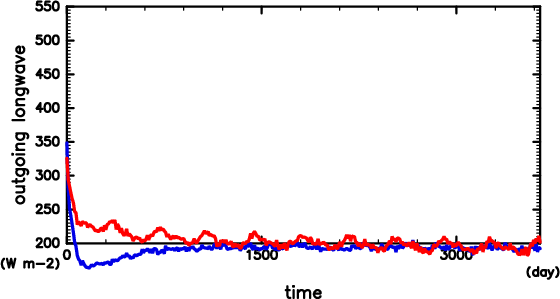
\includegraphics[width=\textwidth]{S1600/S1600_OLRA-OSRA_horimean_time0.0-3650.0-crop.png}
			\(S=1600\hmu{W/m^2}\)\\
			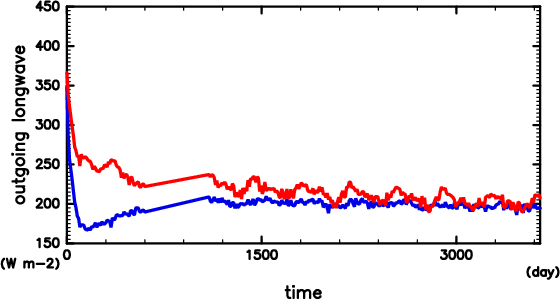
\includegraphics[width=\textwidth]{S1800/S1800_OLRA-OSRA_horimean_time0.0-3650.0-crop.png}
			\(S=1800\hmu{W/m^2}\)
		\end{column}
		\begin{column}{.3\textwidth}
			\centering
			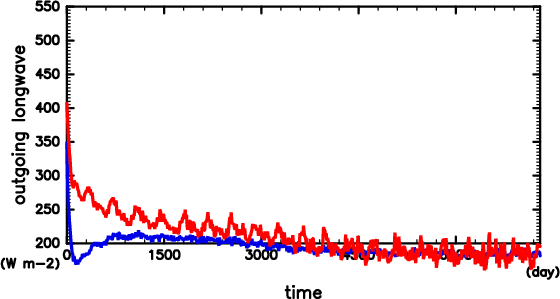
\includegraphics[width=\textwidth]{S2000/S2000_OLRA-OSRA_horimean_time0.0-7300.0-crop.png}
			\(S=2000\hmu{W/m^2}\)
		\end{column}
	\end{columns}
\end{frame}
%\begin{frame}
%	\frametitle{結果 (OLRA の時間推移)}
%	\begin{columns}[T]
%		\begin{column}{.3\textwidth}
%			\centering
%			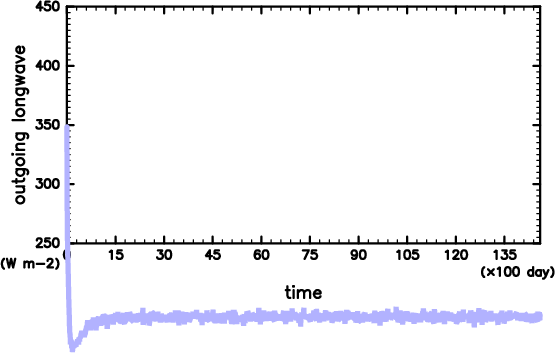
\includegraphics[width=\textwidth]{S1366/S1300_OLRA_horimean_time0.0-14600.0-crop.png}
%			\(S=1366\hmu{W/m^2}\)\\
%			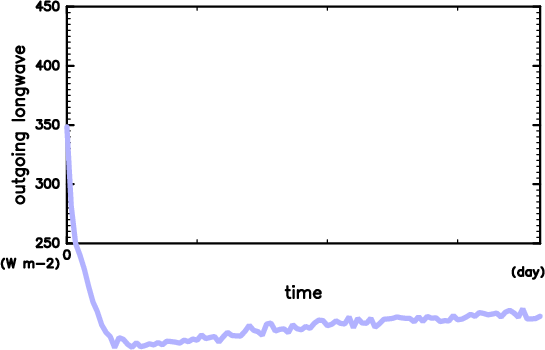
\includegraphics[width=\textwidth]{S1500/S1500_OLRA_horimean_time0.0-1095.0-crop.png}
%			\(S=1500\hmu{W/m^2}\)
%		\end{column}
%		\begin{column}{.3\textwidth}
%			\centering
%			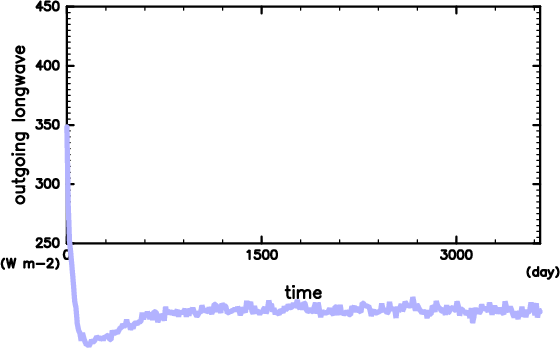
\includegraphics[width=\textwidth]{S1600/S1600_OLRA_horimean_time0.0-3650.0-crop.png}
%			\(S=1600\hmu{W/m^2}\)\\
%			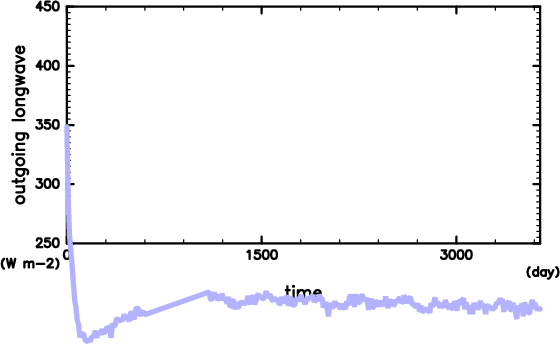
\includegraphics[width=\textwidth]{S1800/S1800_OLRA_horimean_time0.0-3650.0-crop.png}
%			\(S=1800\hmu{W/m^2}\)
%		\end{column}
%		\begin{column}{.3\textwidth}
%			\centering
%			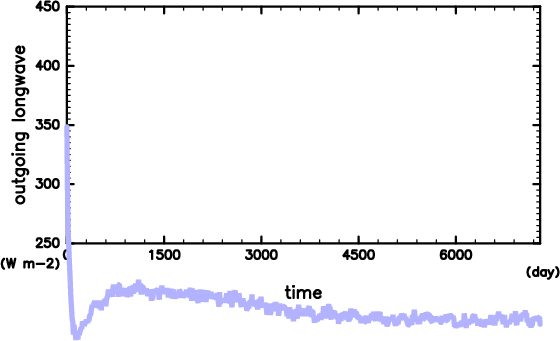
\includegraphics[width=\textwidth]{S2000/S2000_OLRA_horimean_time0.0-7300.0-crop.png}
%			\(S=2000\hmu{W/m^2}\)
%		\end{column}
%	\end{columns}
%\end{frame}

\begin{frame}
	\frametitle{結果 (地表面温度; 計算終了年での平均)}
	\begin{columns}[T]
		\begin{column}{.3\textwidth}
			\centering
			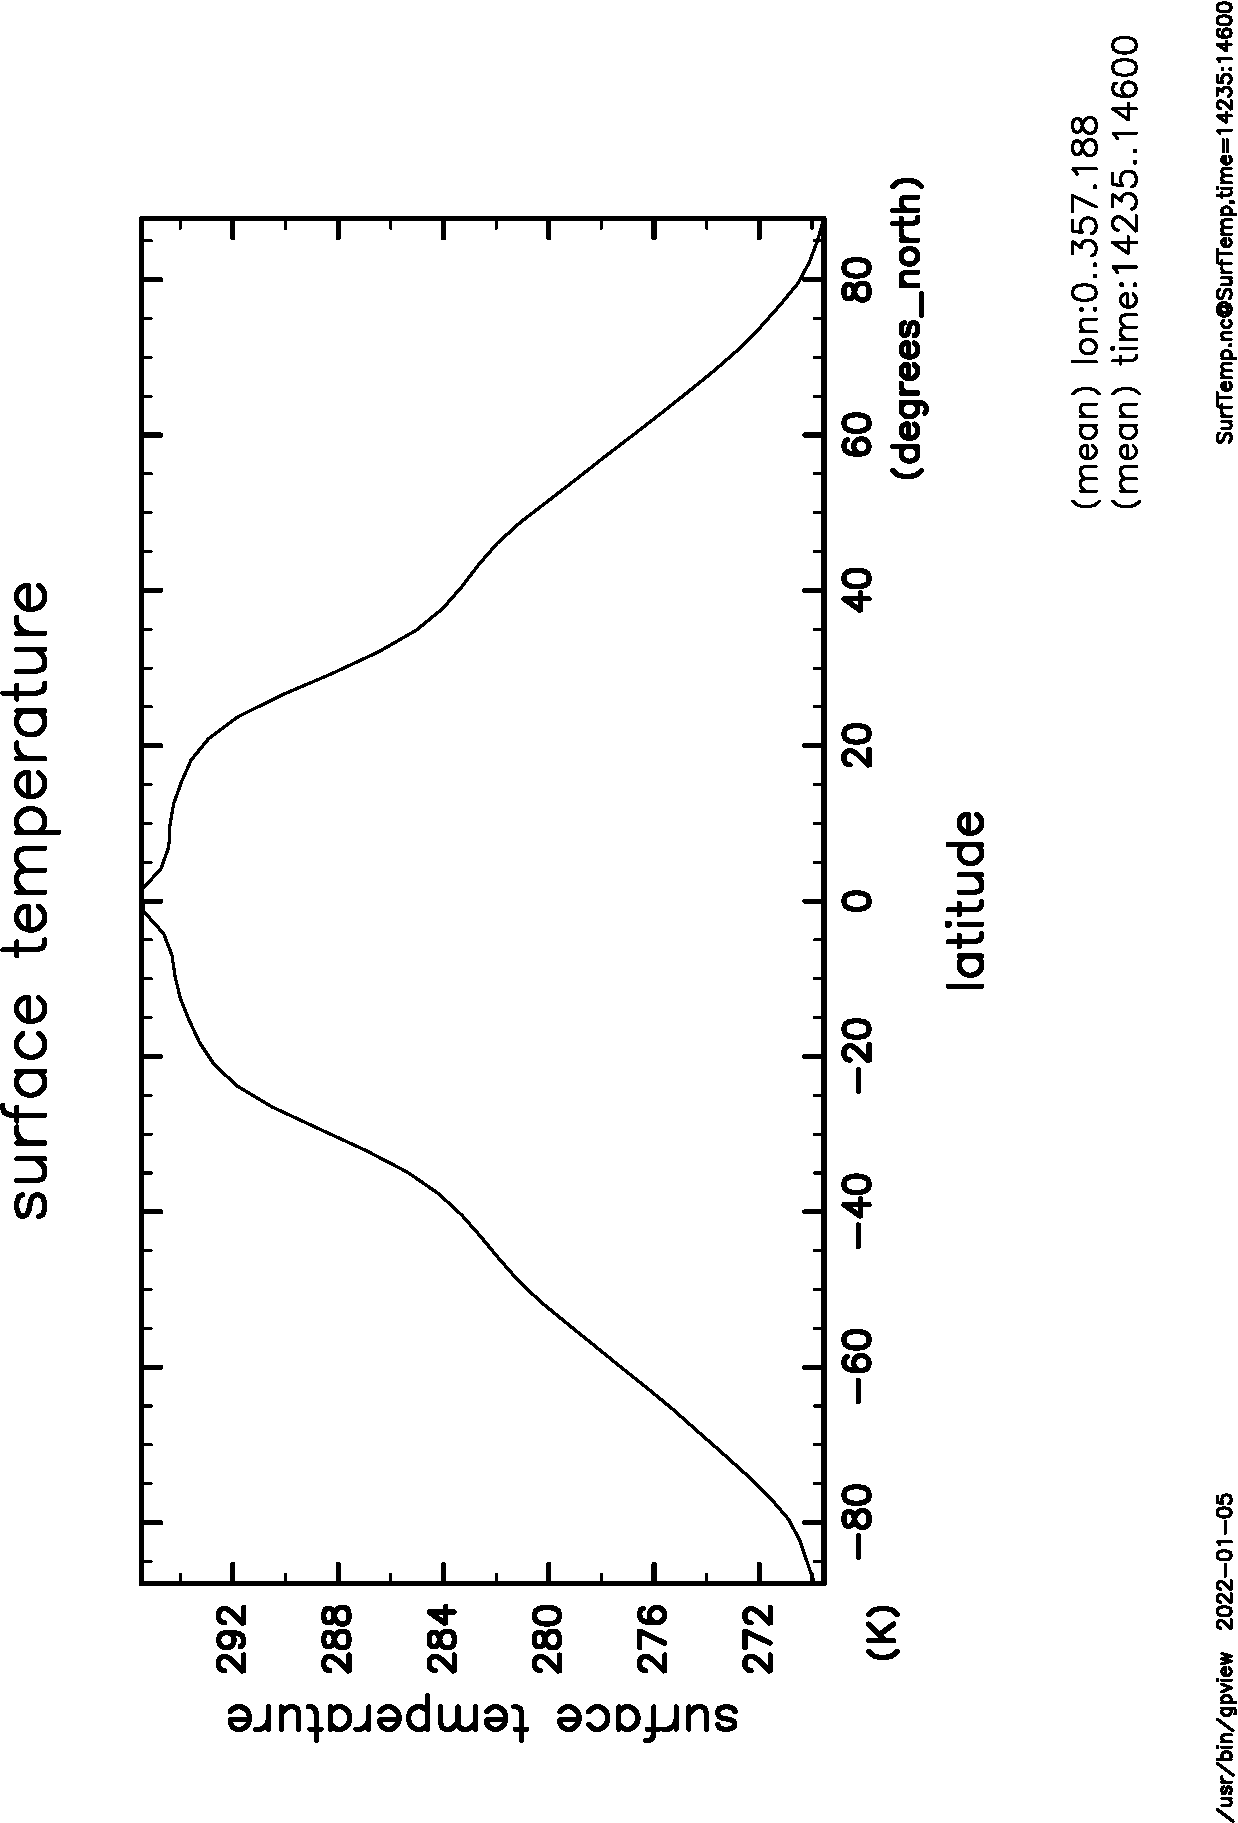
\includegraphics[height=\textwidth,angle=-90]{S1366/SurfTemp,time=14235:14600-crop.pdf}
			\(S=1366\hmu{W/m^2}\)\\
			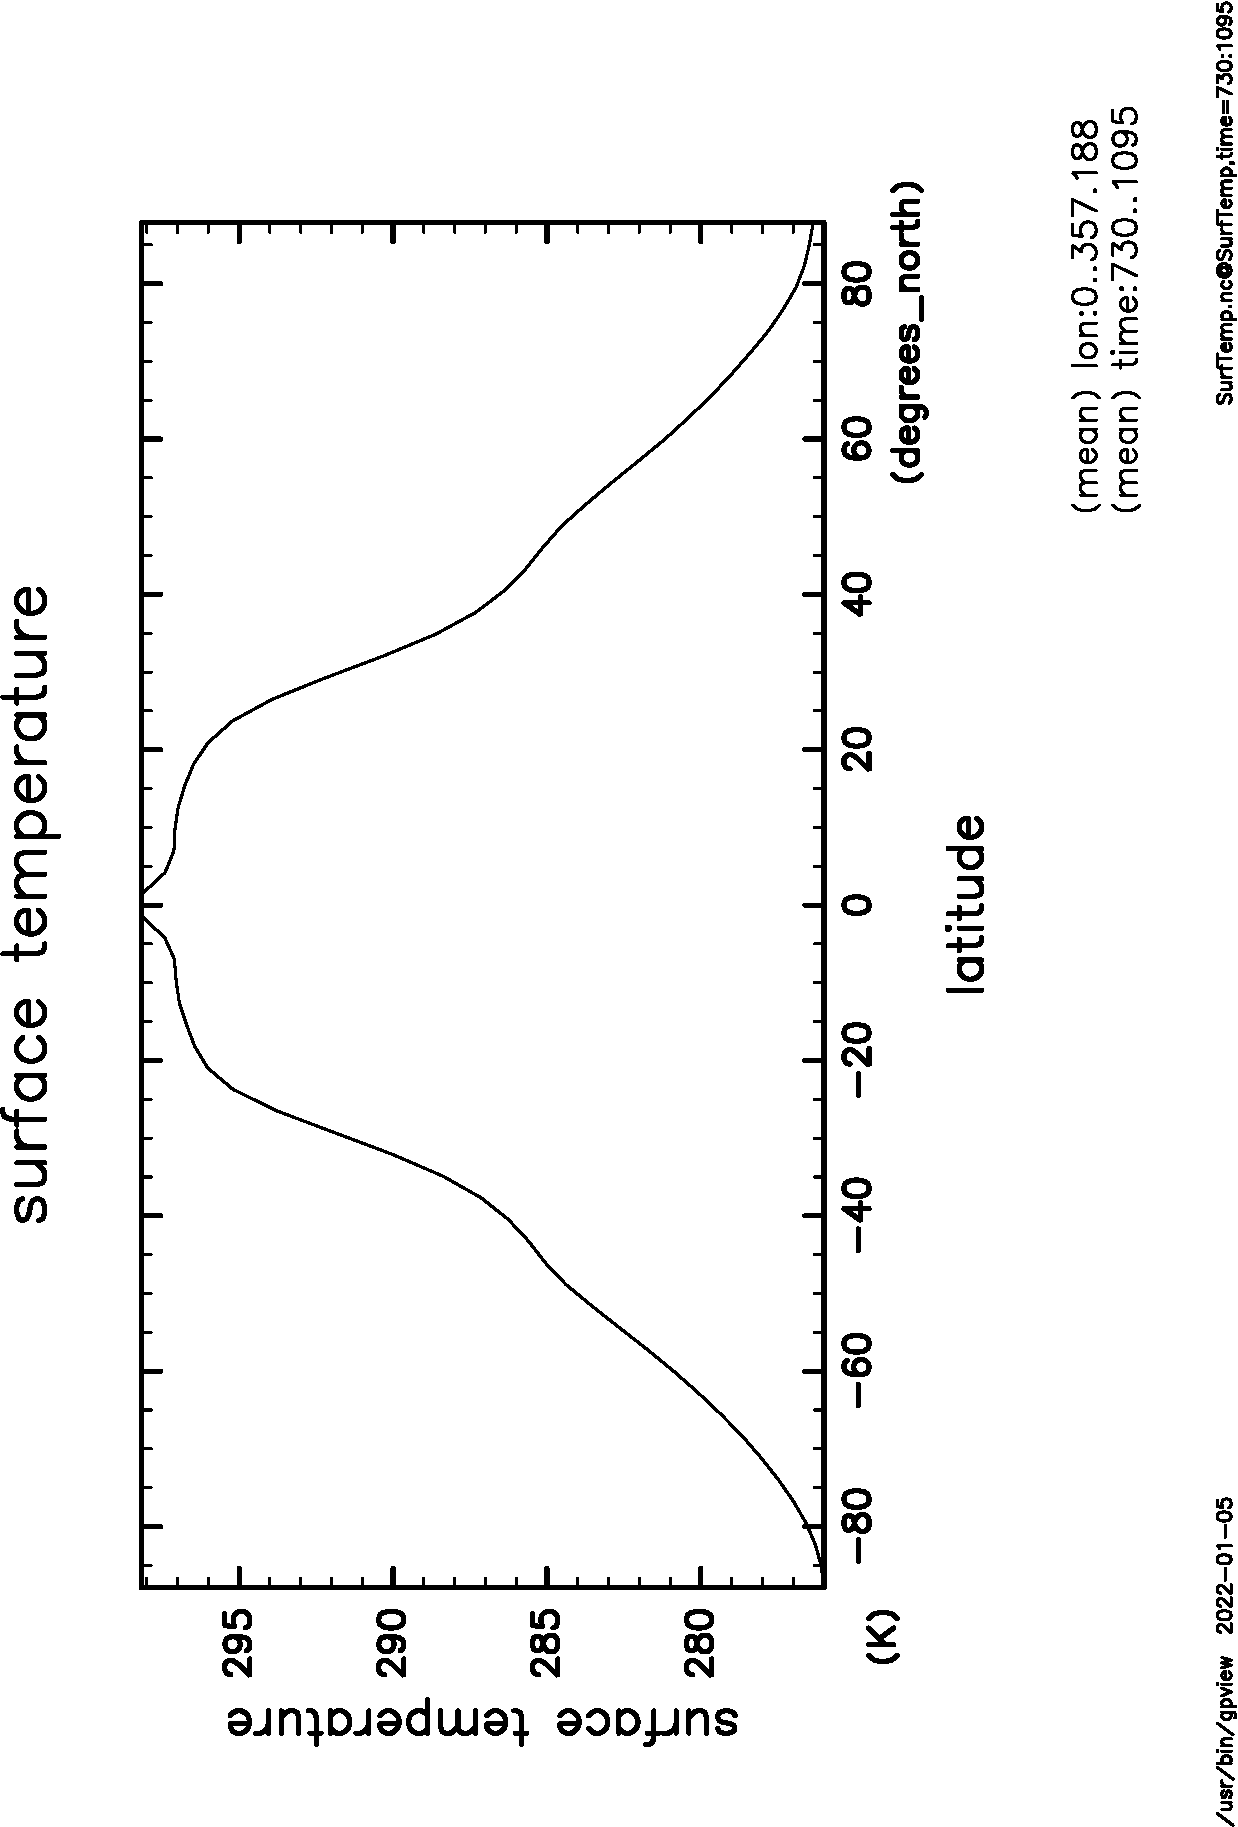
\includegraphics[height=\textwidth,angle=-90]{S1500/SurfTemp,time=730:1095-crop.pdf}
			\(S=1500\hmu{W/m^2}\)
		\end{column}
		\begin{column}{.3\textwidth}
			\centering
			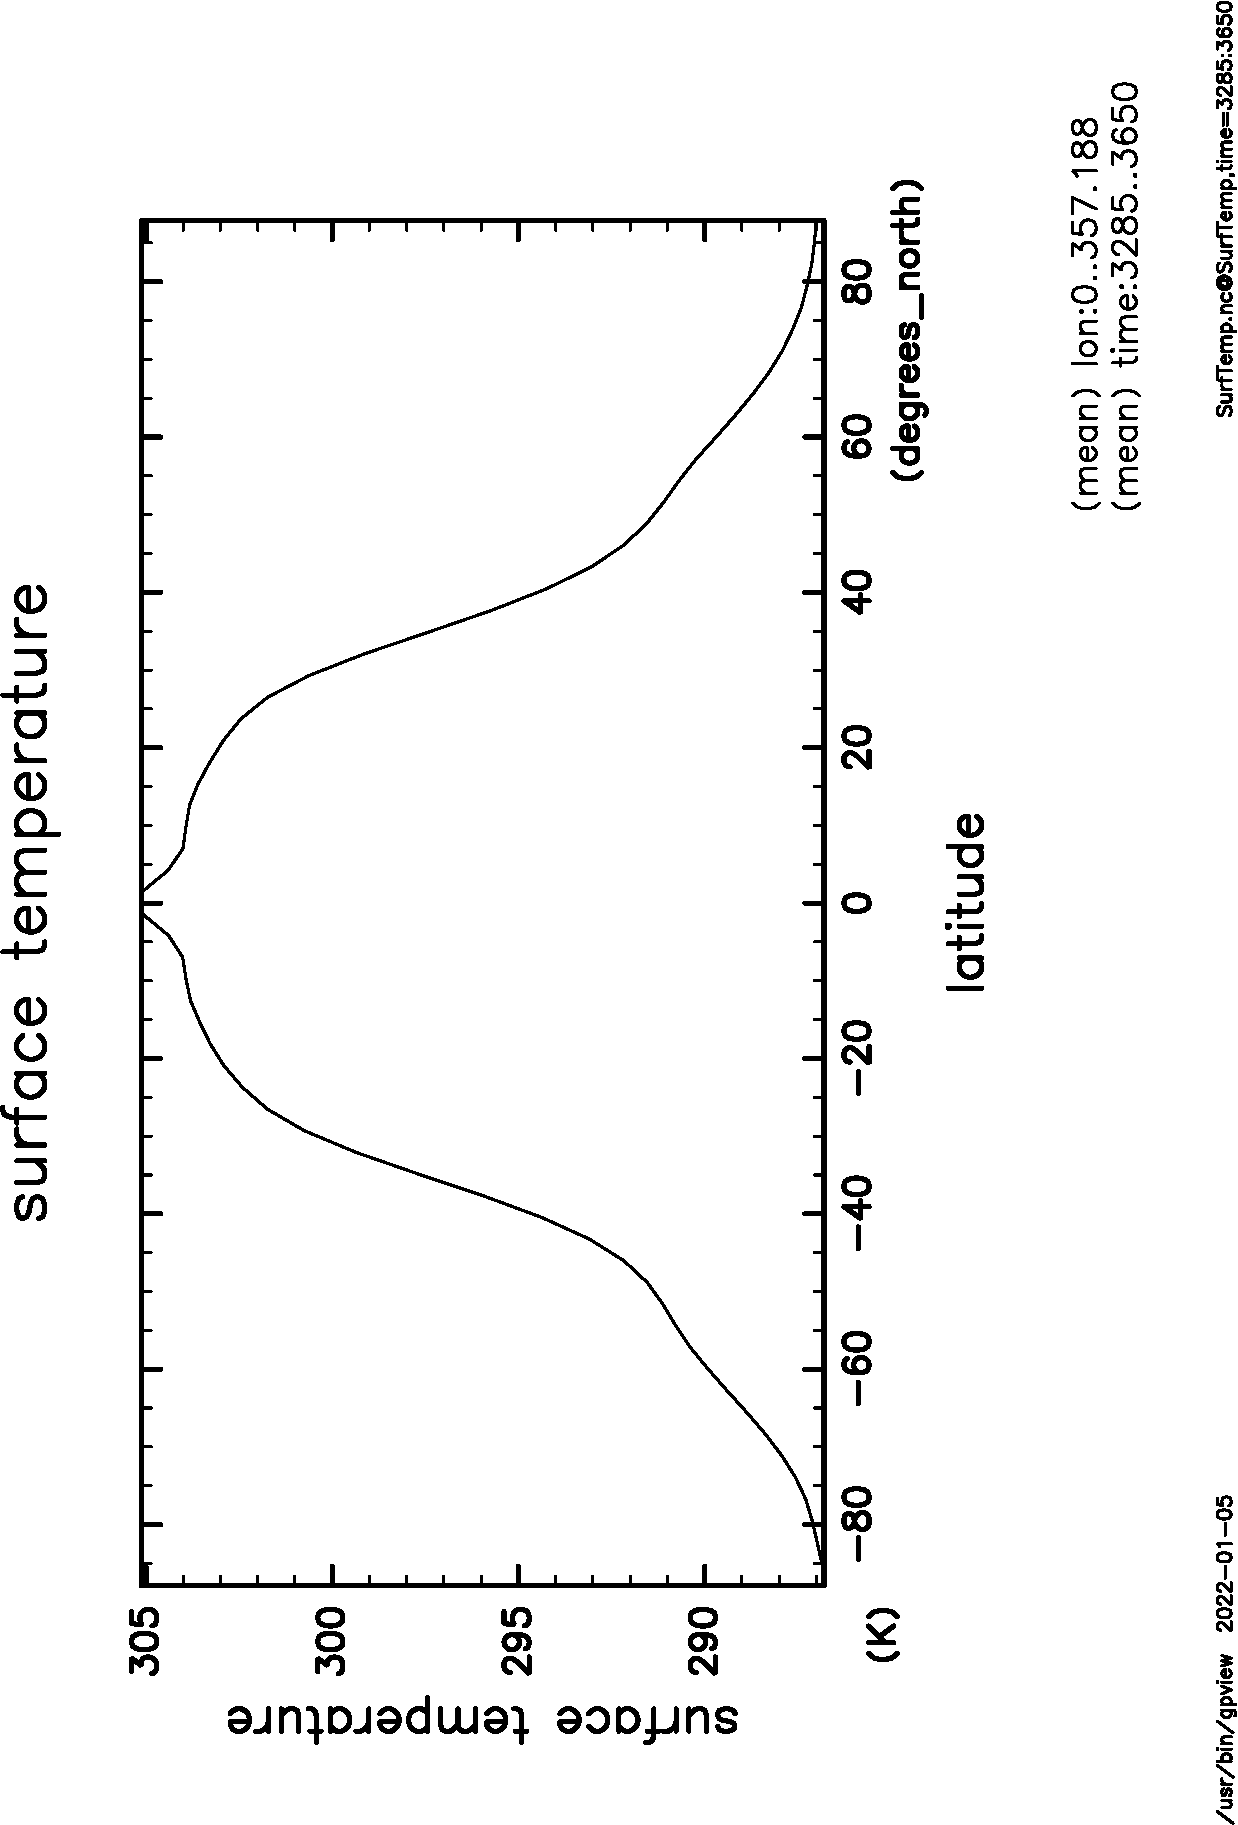
\includegraphics[height=\textwidth,angle=-90]{S1600/SurfTemp,time=3285:3650-crop.pdf}
			\(S=1600\hmu{W/m^2}\)\\
			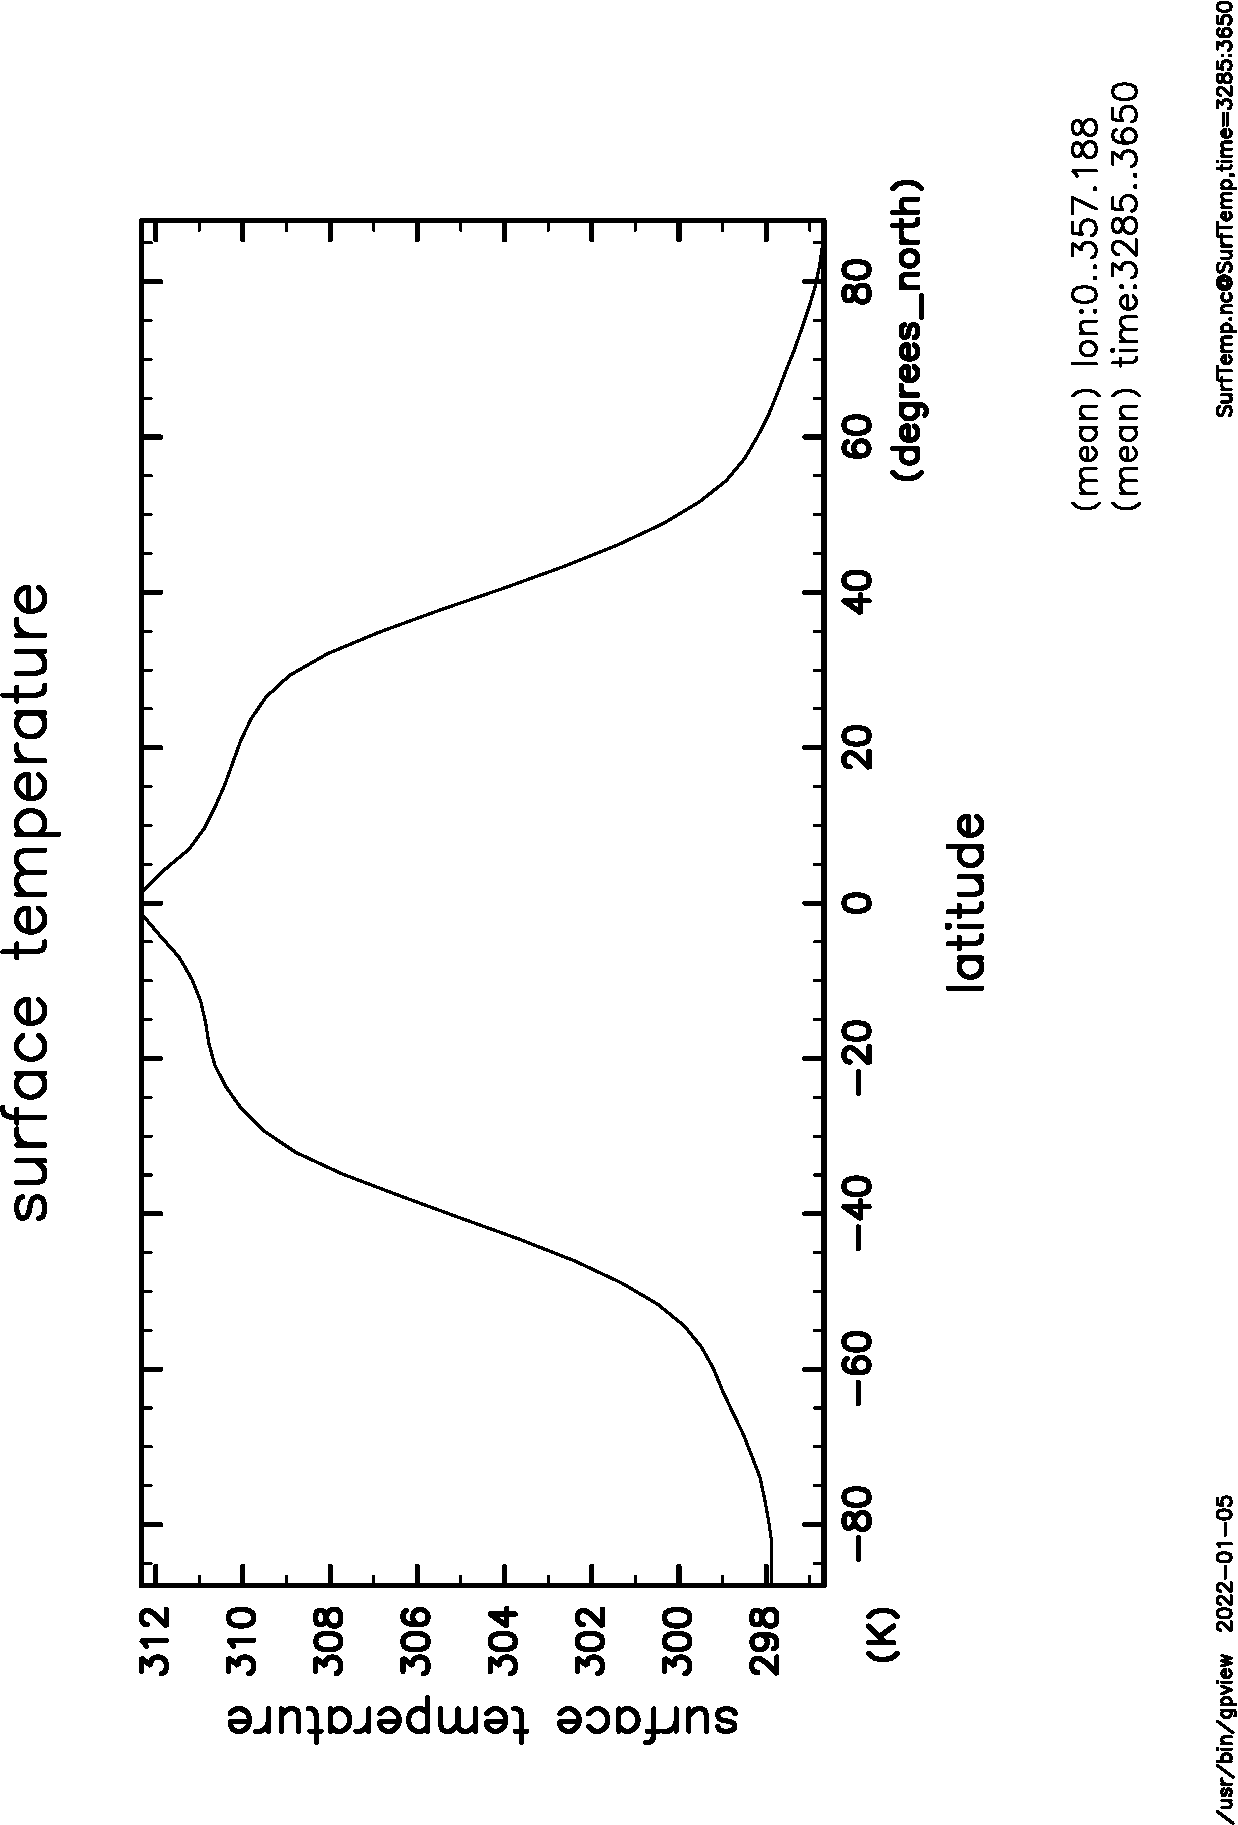
\includegraphics[height=\textwidth,angle=-90]{S1800/SurfTemp,time=3285:3650-crop.pdf}
			\(S=1800\hmu{W/m^2}\)
		\end{column}
		\begin{column}{.3\textwidth}
			\centering
			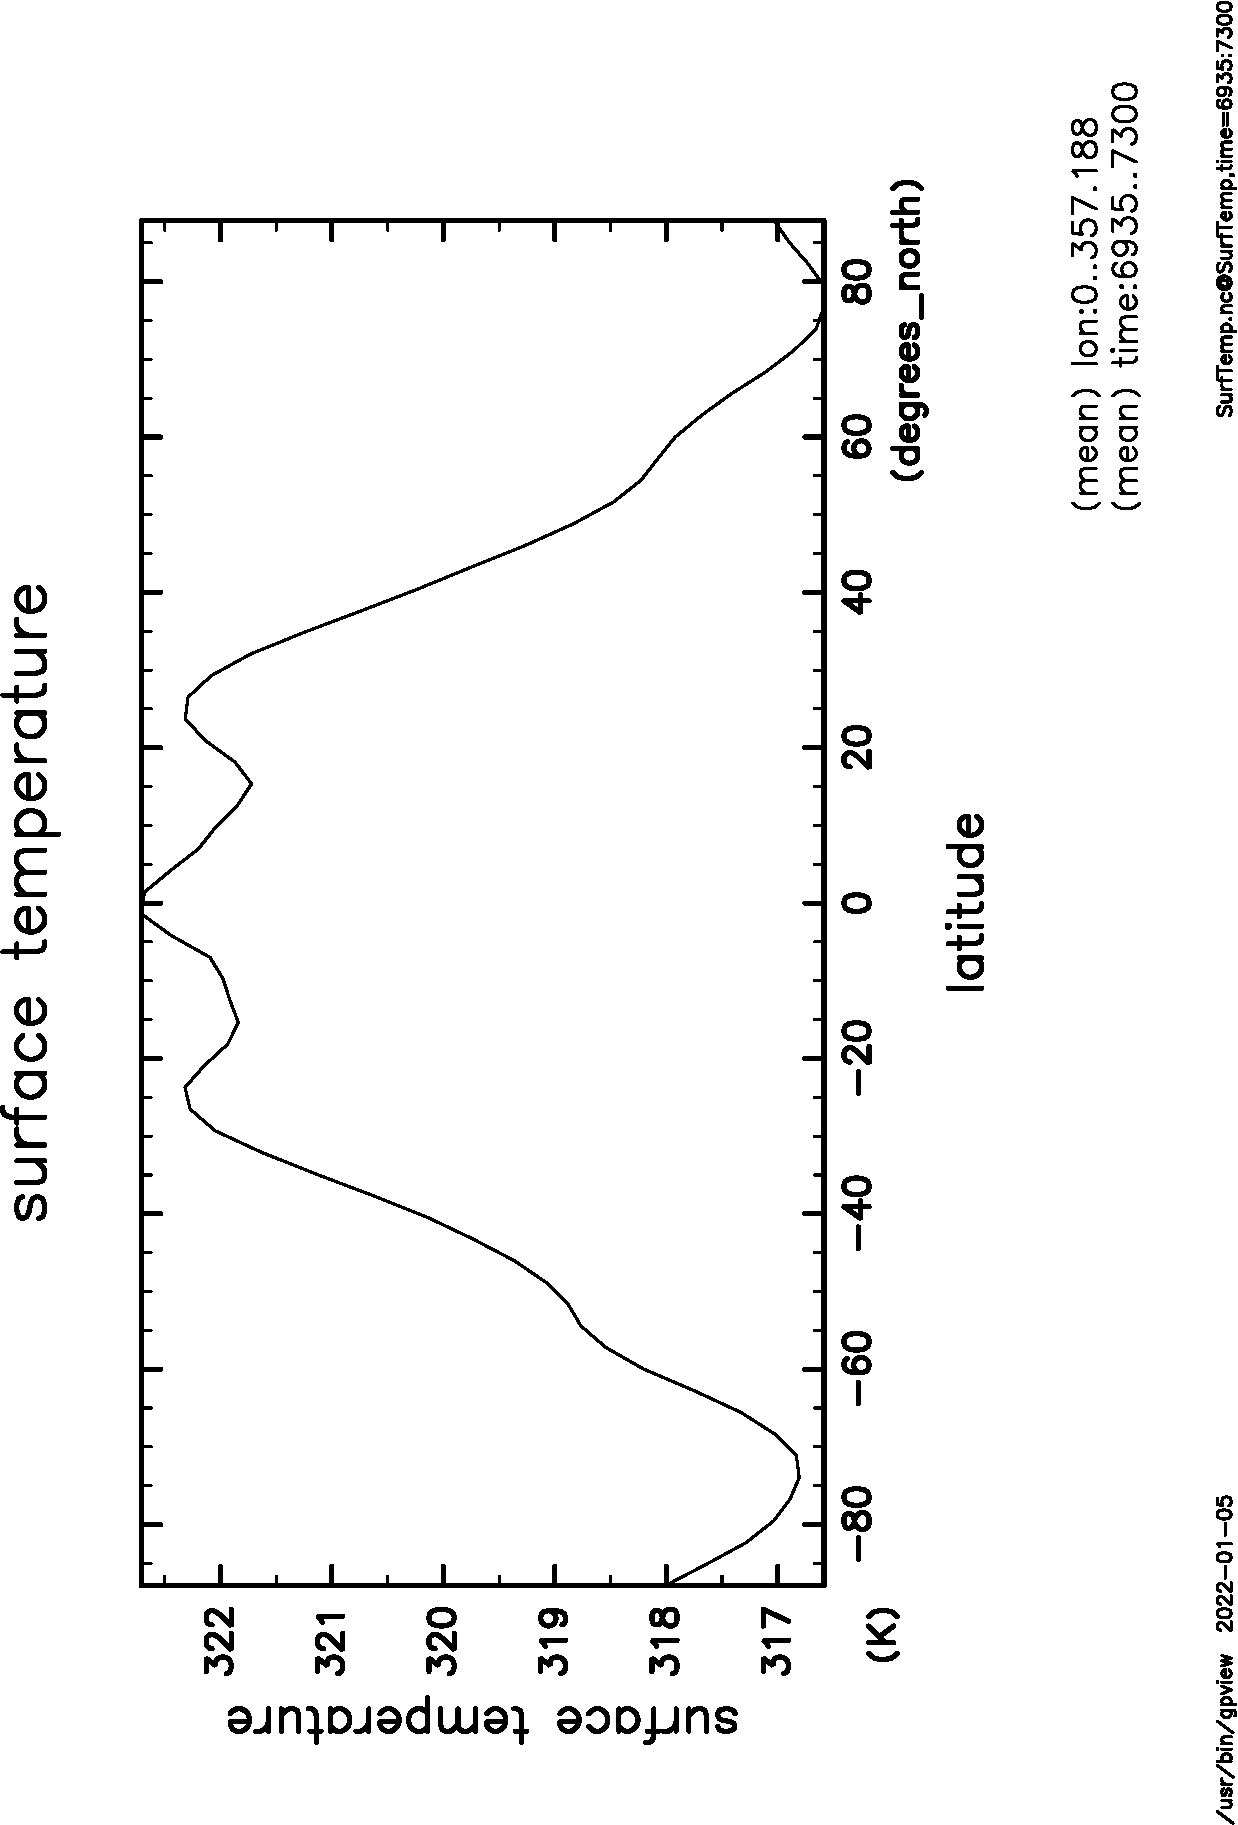
\includegraphics[height=\textwidth,angle=-90]{S2000/SurfTemp,time=6935:7300-crop.pdf}
			\(S=2000\hmu{W/m^2}\)
		\end{column}
	\end{columns}
\end{frame}

\begin{frame}
	\frametitle{結果 (東西風; 計算終了年での平均)}
	\begin{columns}[T]
		\begin{column}{.3\textwidth}
			\centering
			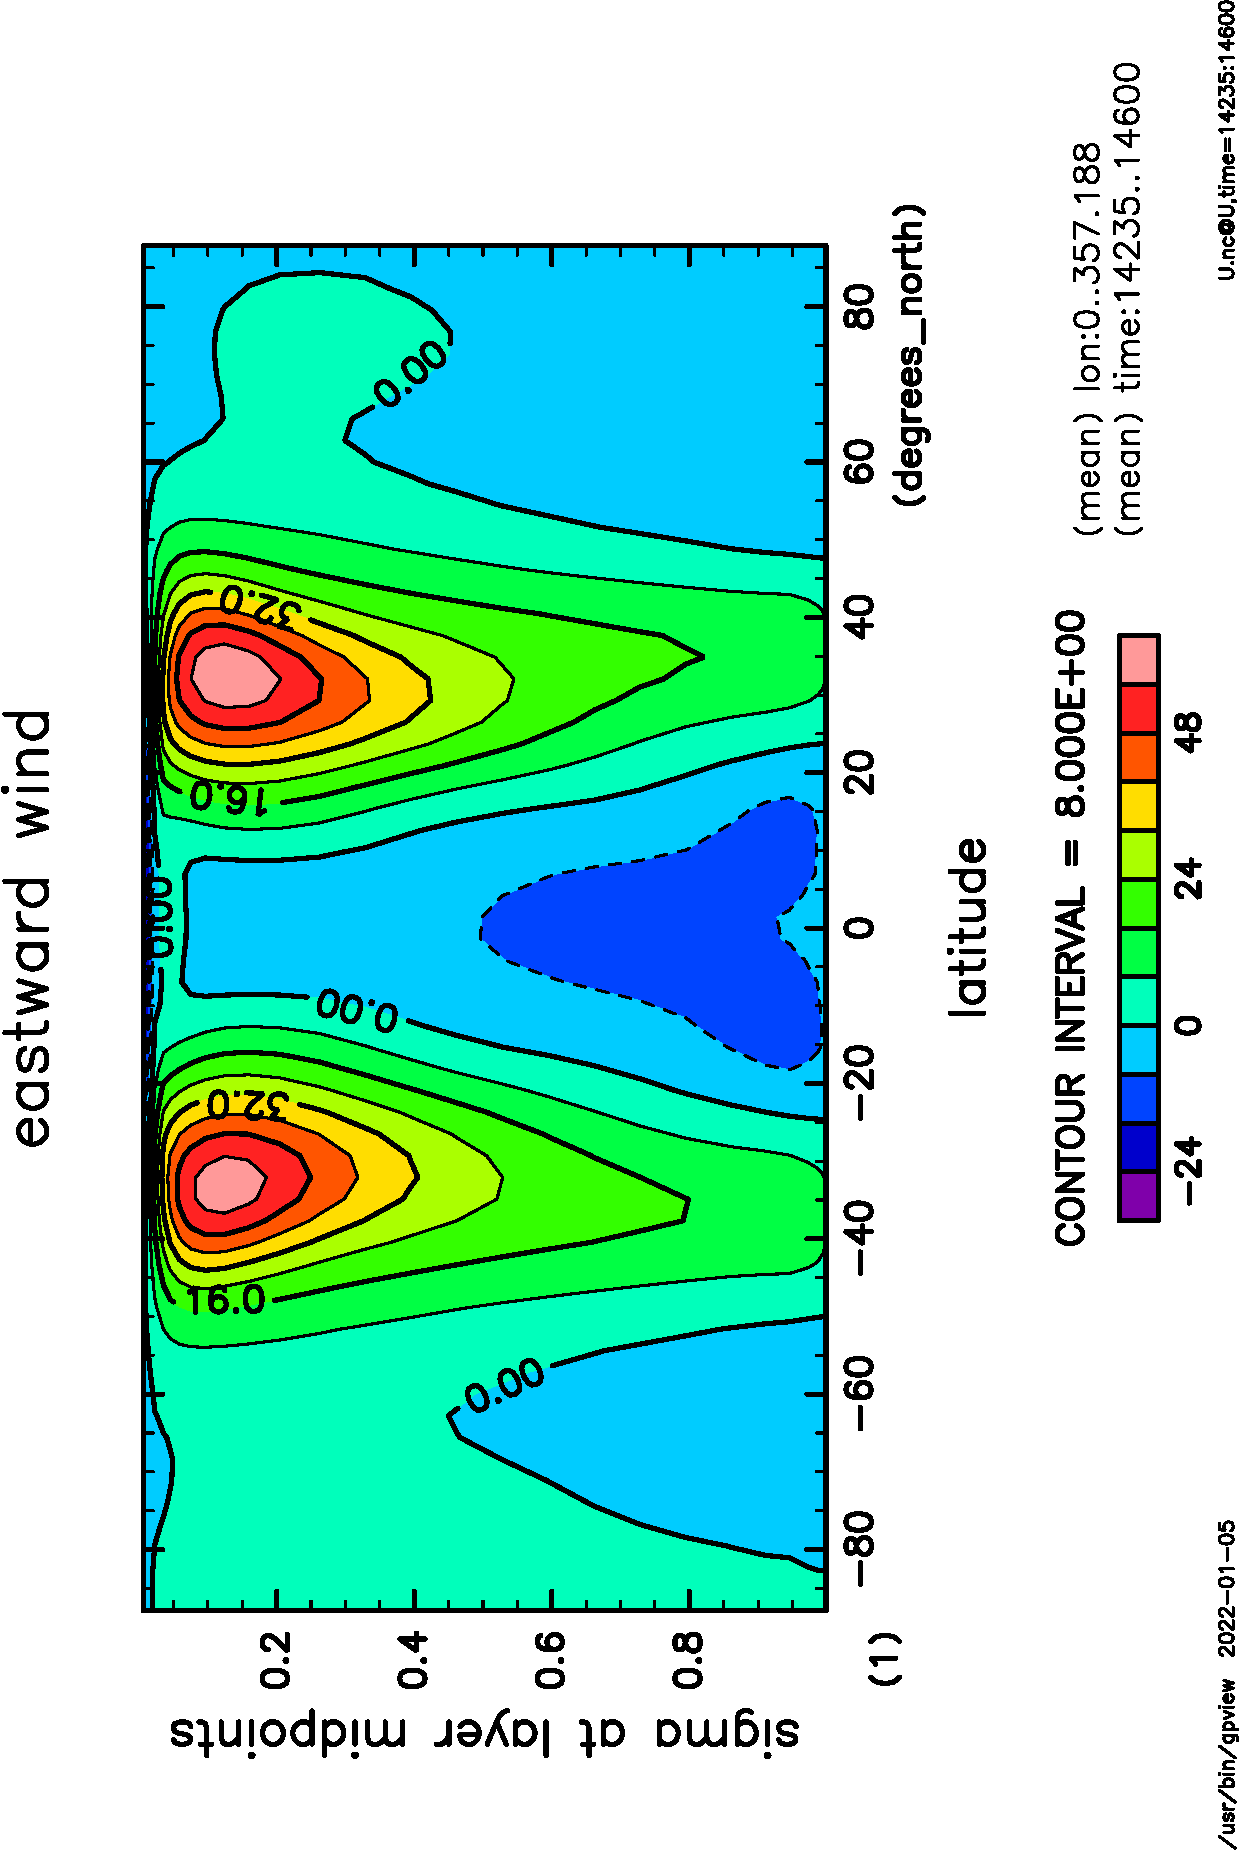
\includegraphics[height=\textwidth,angle=-90]{S1366/U,time=14235:14600-crop.pdf}
			\(S=1366\hmu{W/m^2}\)\\
			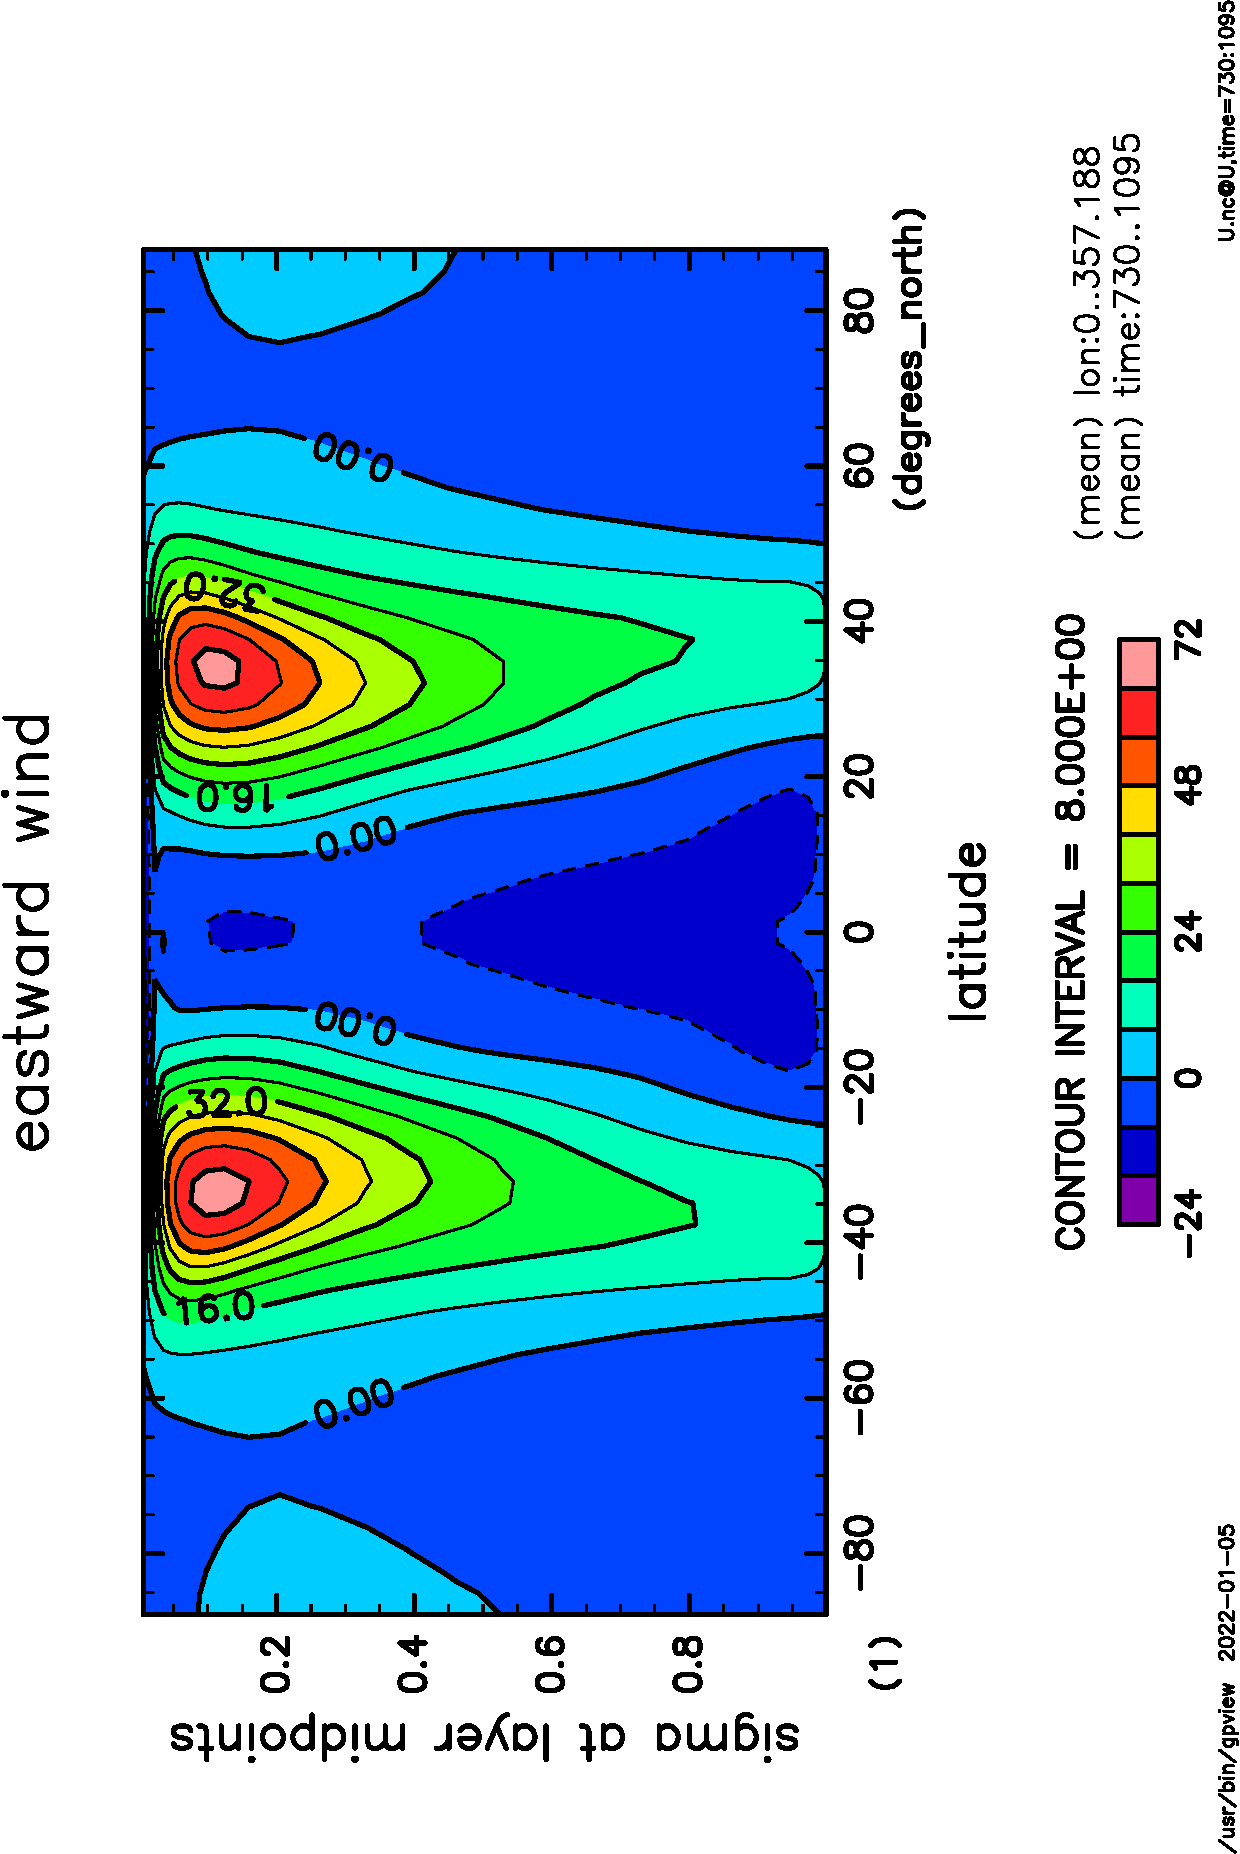
\includegraphics[height=\textwidth,angle=-90]{S1500/U,time=730:1095-crop.pdf}
			\(S=1500\hmu{W/m^2}\)
		\end{column}
		\begin{column}{.3\textwidth}
			\centering
			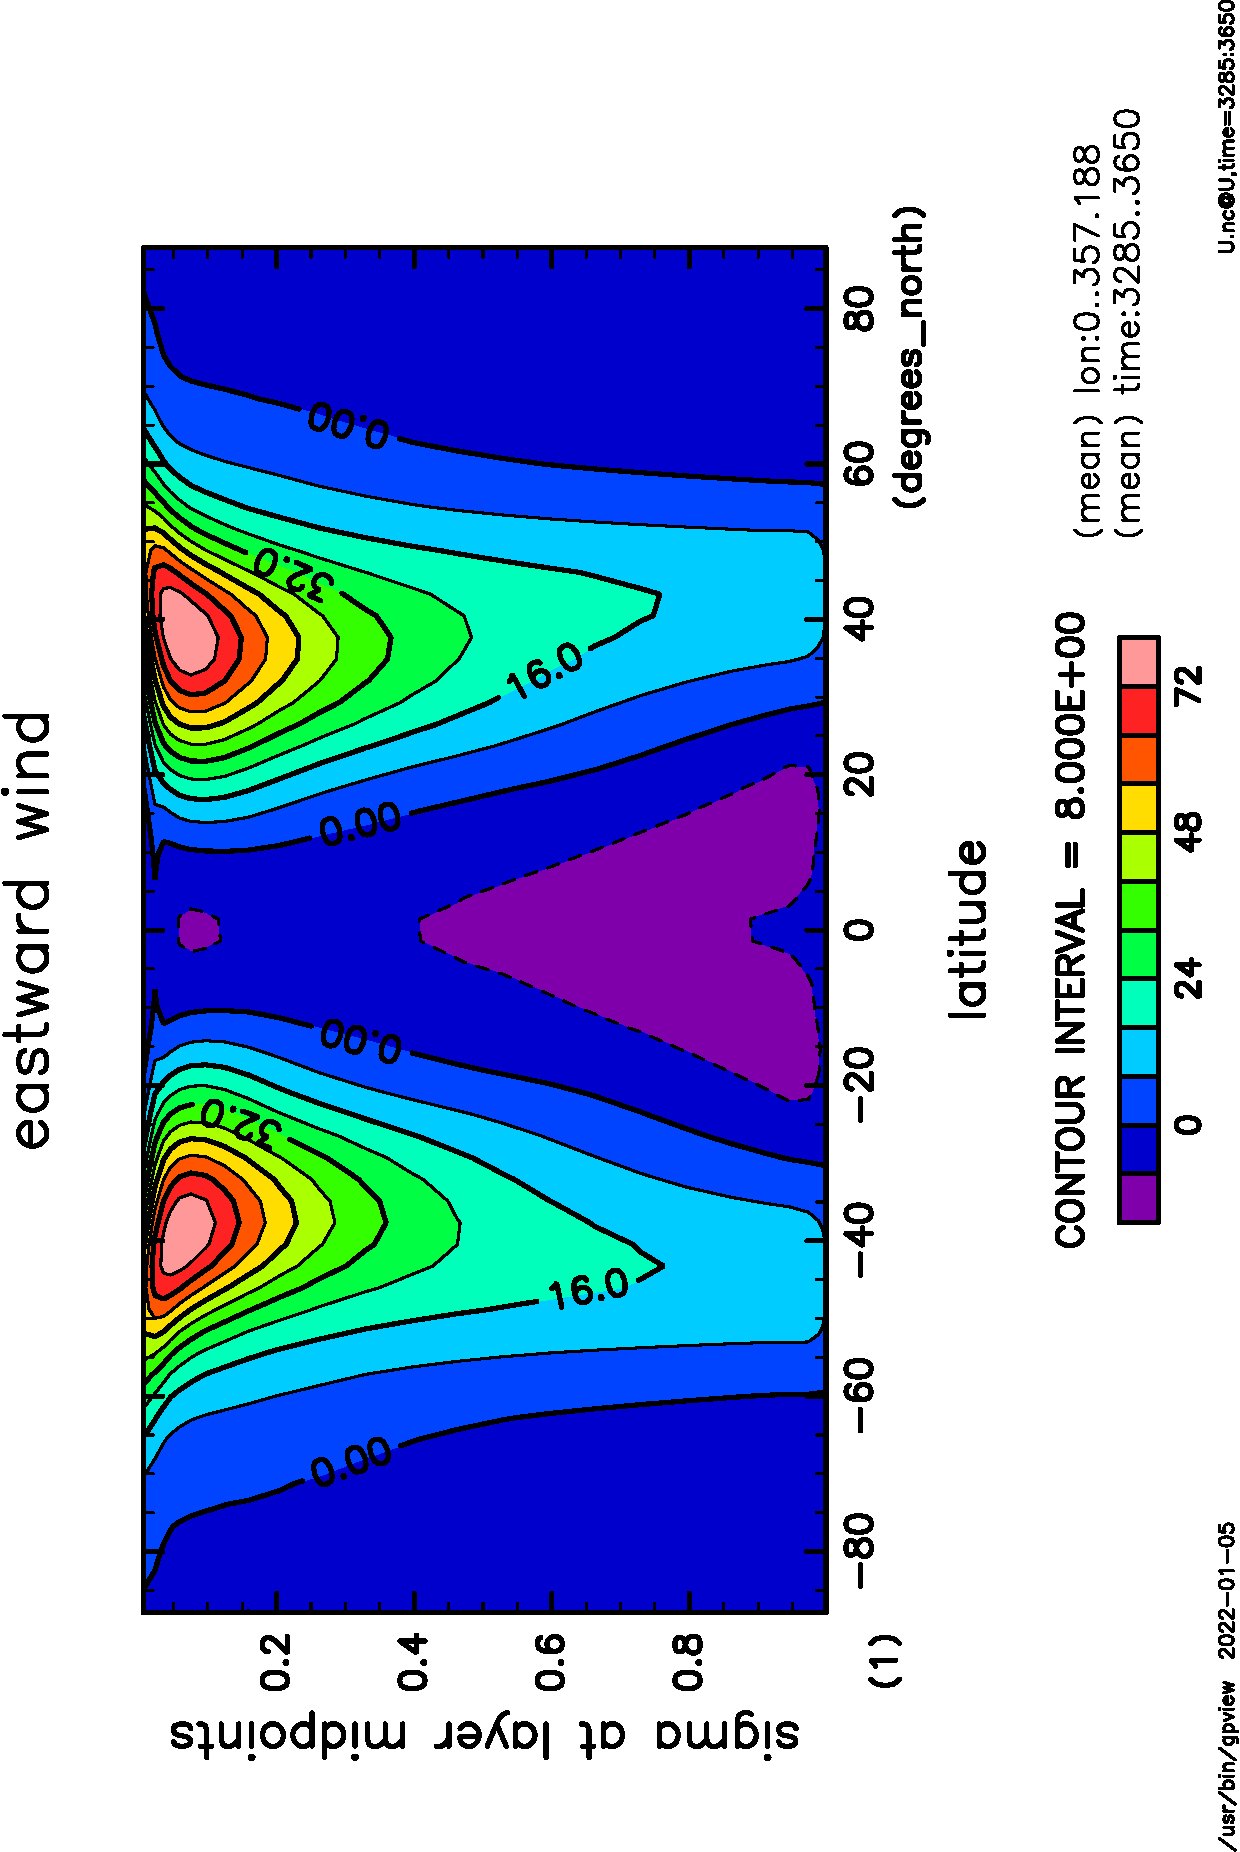
\includegraphics[height=\textwidth,angle=-90]{S1600/U,time=3285:3650-crop.pdf}
			\(S=1600\hmu{W/m^2}\)\\
			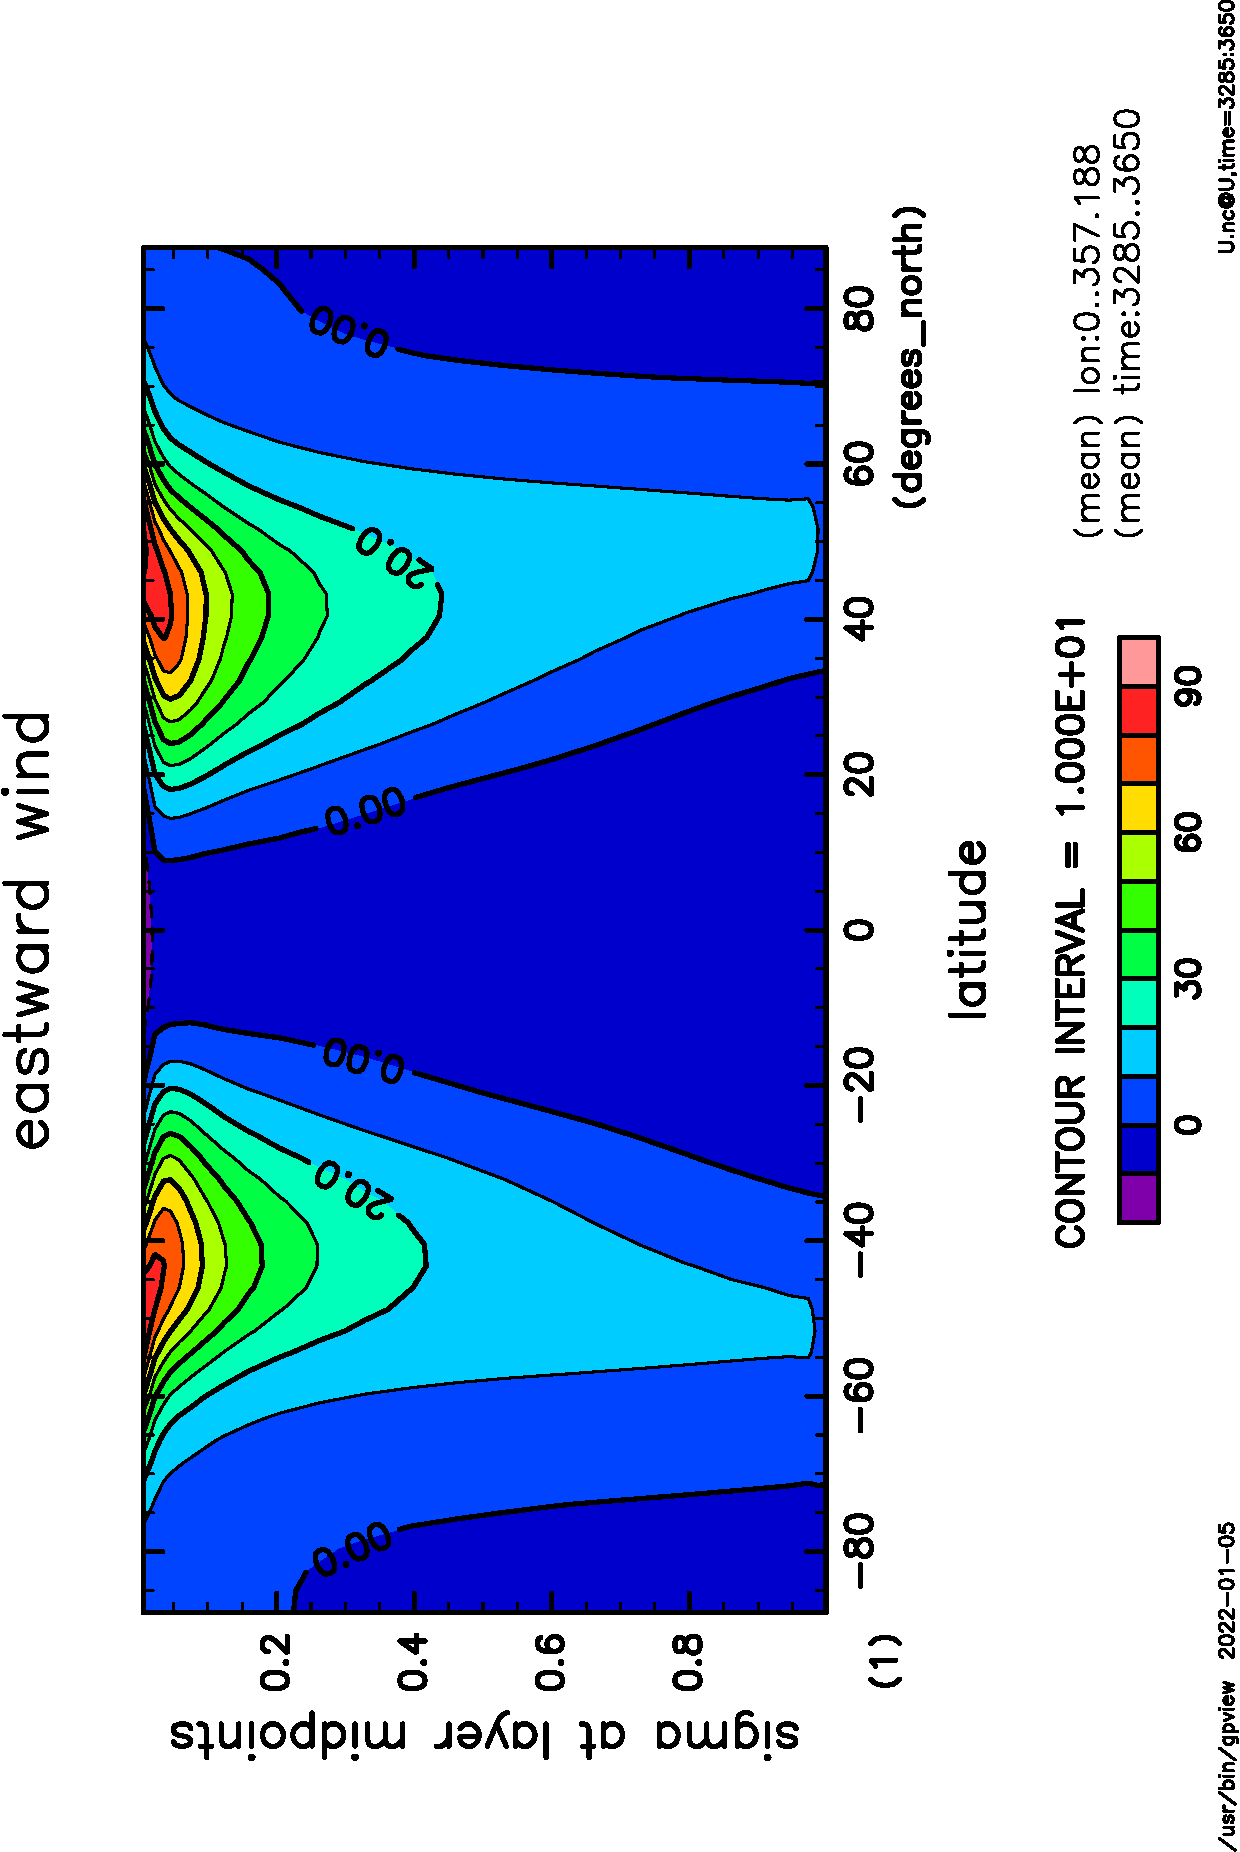
\includegraphics[height=\textwidth,angle=-90]{S1800/U,time=3285:3650-crop.pdf}
			\(S=1800\hmu{W/m^2}\)
		\end{column}
		\begin{column}{.3\textwidth}
			\centering
			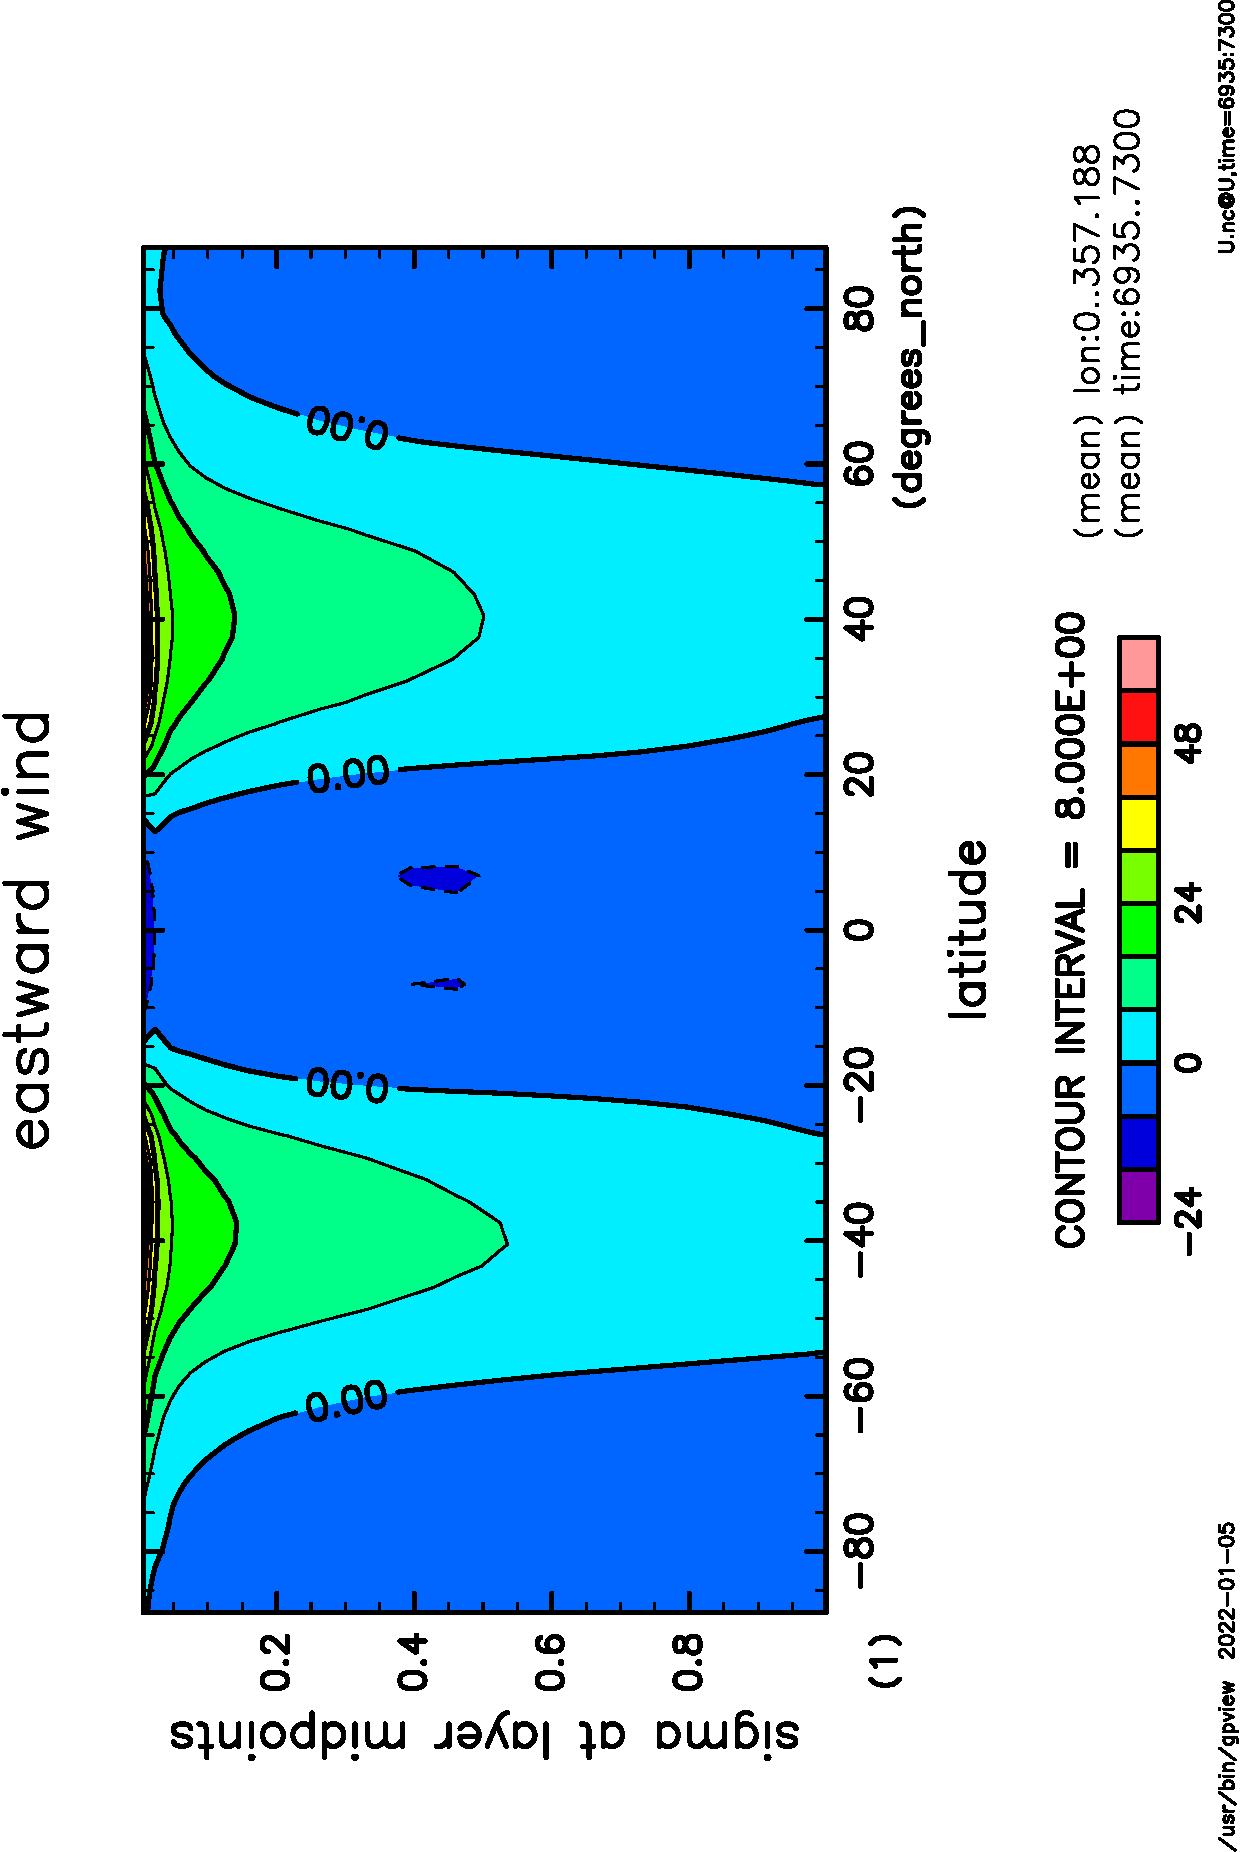
\includegraphics[height=\textwidth,angle=-90]{S2000/U,time=6935:7300-crop.pdf}
			\(S=2000\hmu{W/m^2}\)
		\end{column}
	\end{columns}
\end{frame}

\begin{frame}
	\frametitle{南北熱輸送}
	\begin{gather*}
		\mathrm{latentEnFlxLat}=\int Lqv\,dp\tag{潜熱輸送}\\
		\mathrm{dryStatEnFlxLat}=\int (C_pT+gh)v\,dp\tag{乾燥静的エネルギー}\\
		\mathrm{moistStatEnFlxLat}=(\mathrm{dryStatEnFlxLat}+\mathrm{latentEn})\tag{湿潤静的エネルギー}
	\end{gather*}
\end{frame}

\begin{frame}
	\frametitle{結果 (南北熱輸送; 計算終了年での平均)}
	\begin{columns}[T]
		\begin{column}{.3\textwidth}
			\centering
			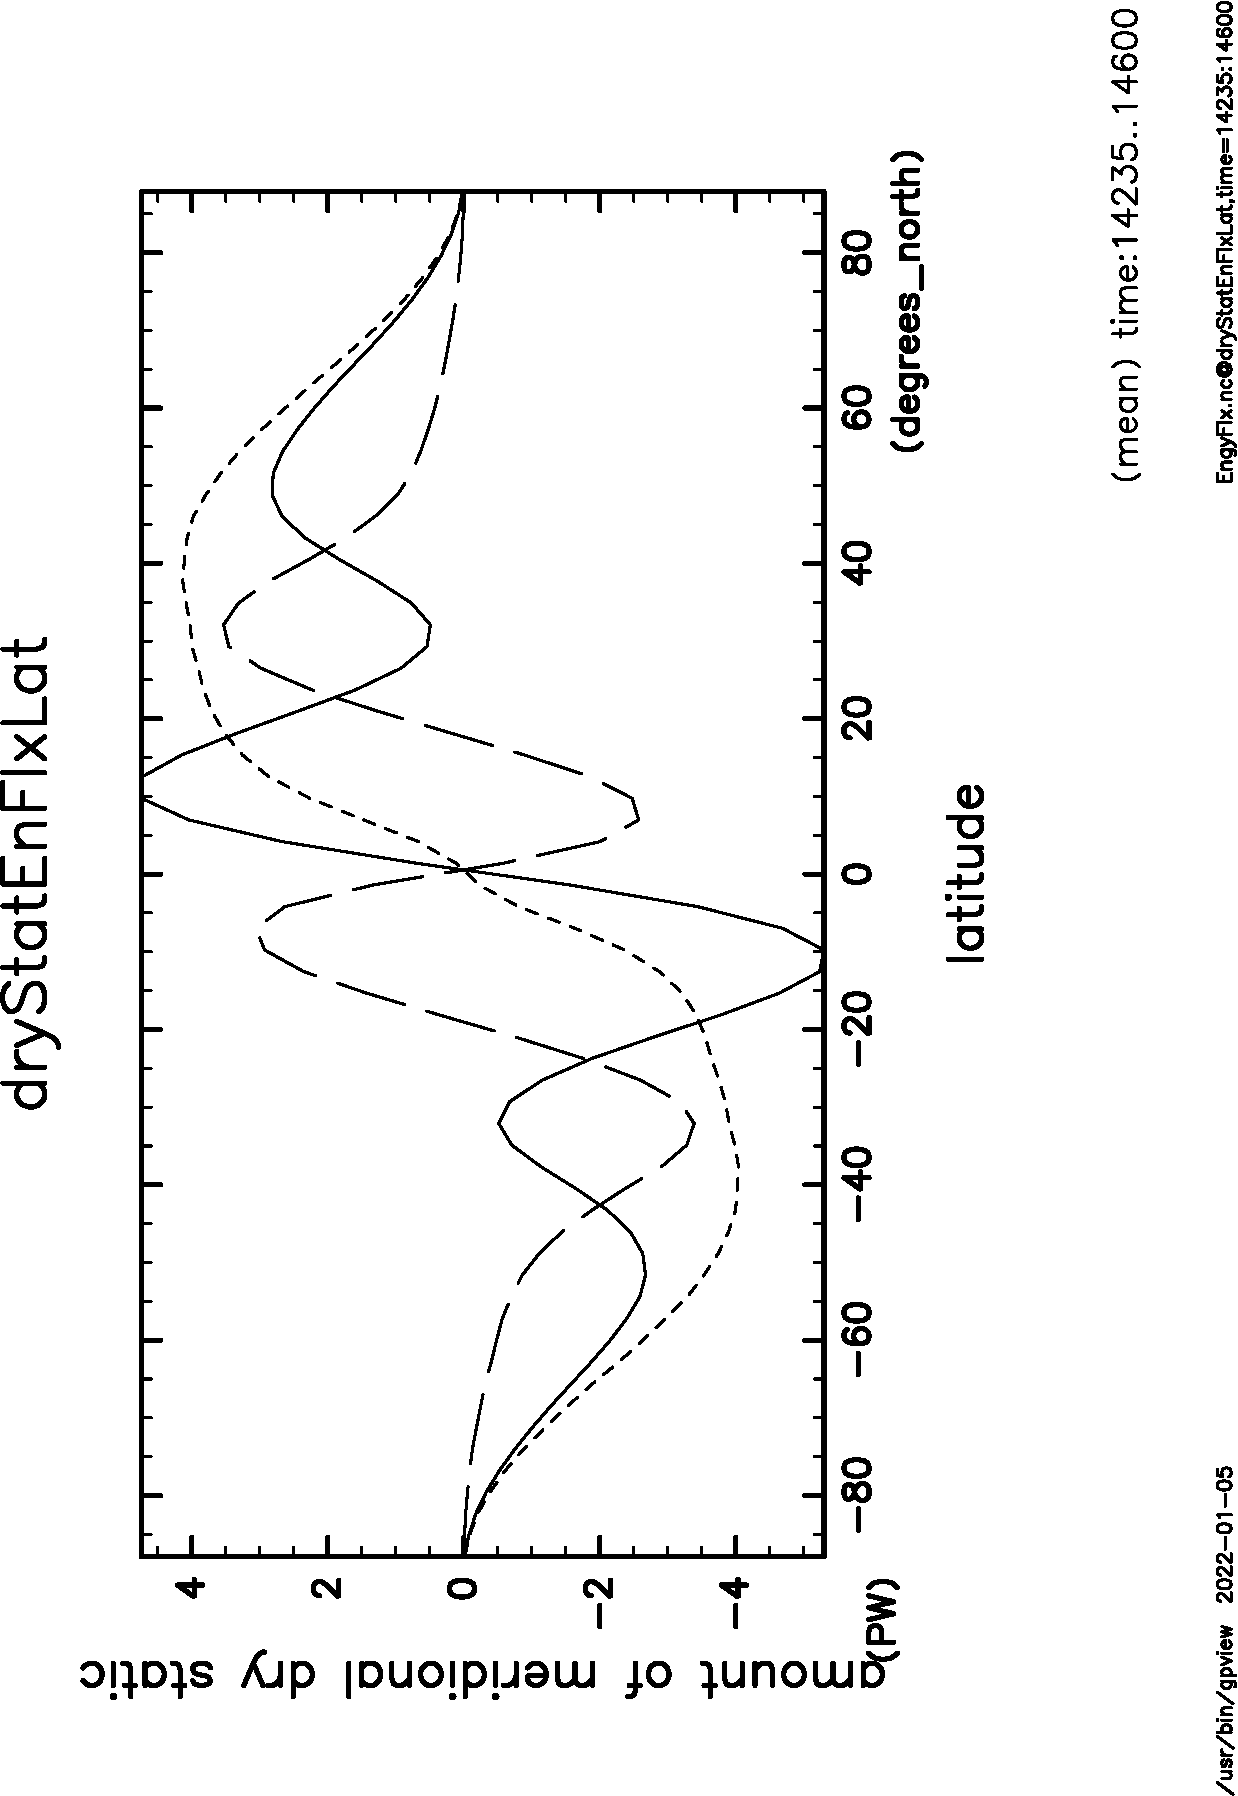
\includegraphics[height=\textwidth,angle=-90]{S1366/EngyFlx,time=14235:14600-crop.pdf}
			\(S=1366\hmu{W/m^2}\)\\
			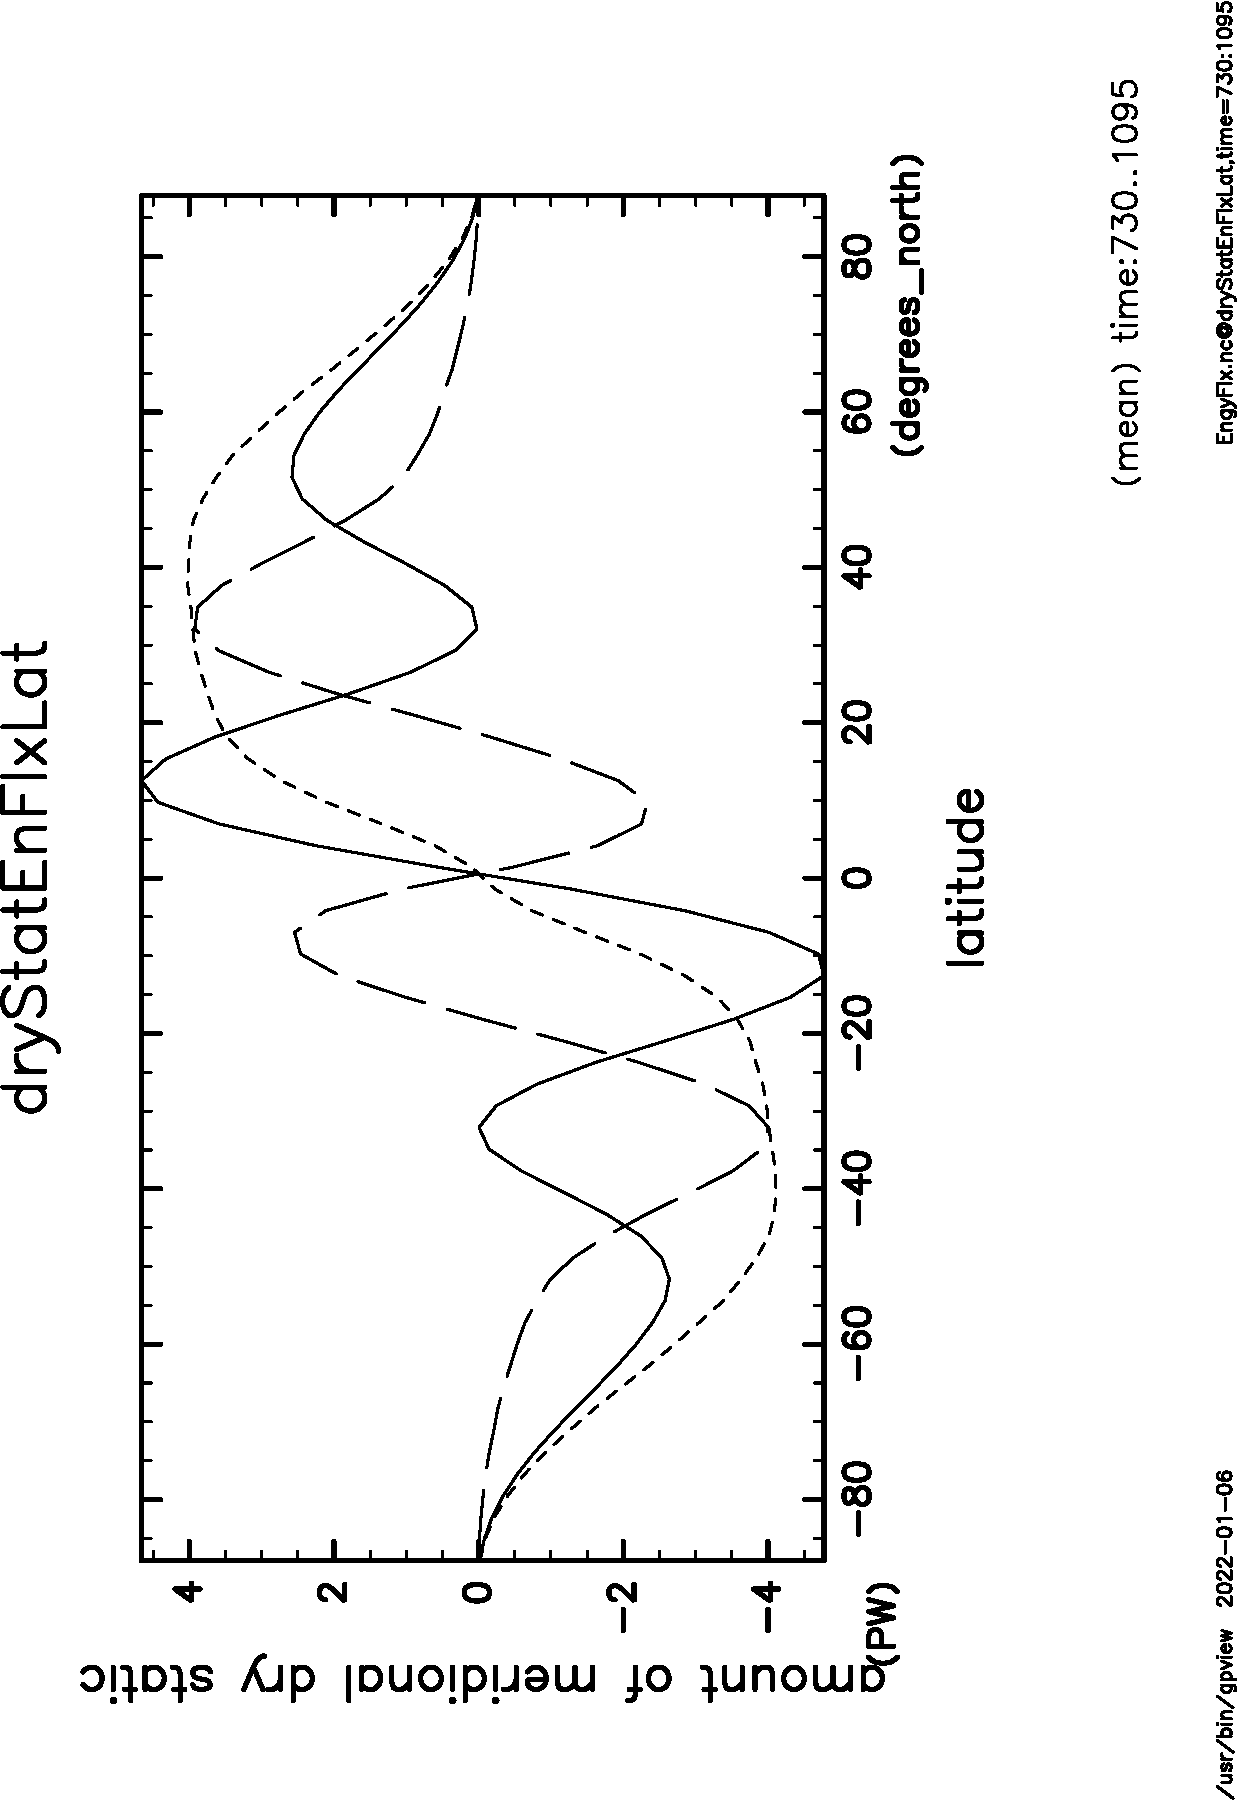
\includegraphics[height=\textwidth,angle=-90]{S1500/EngyFlx,time=730:1095-crop.pdf}
			\(S=1500\hmu{W/m^2}\)
		\end{column}
		\begin{column}{.3\textwidth}
			\centering
			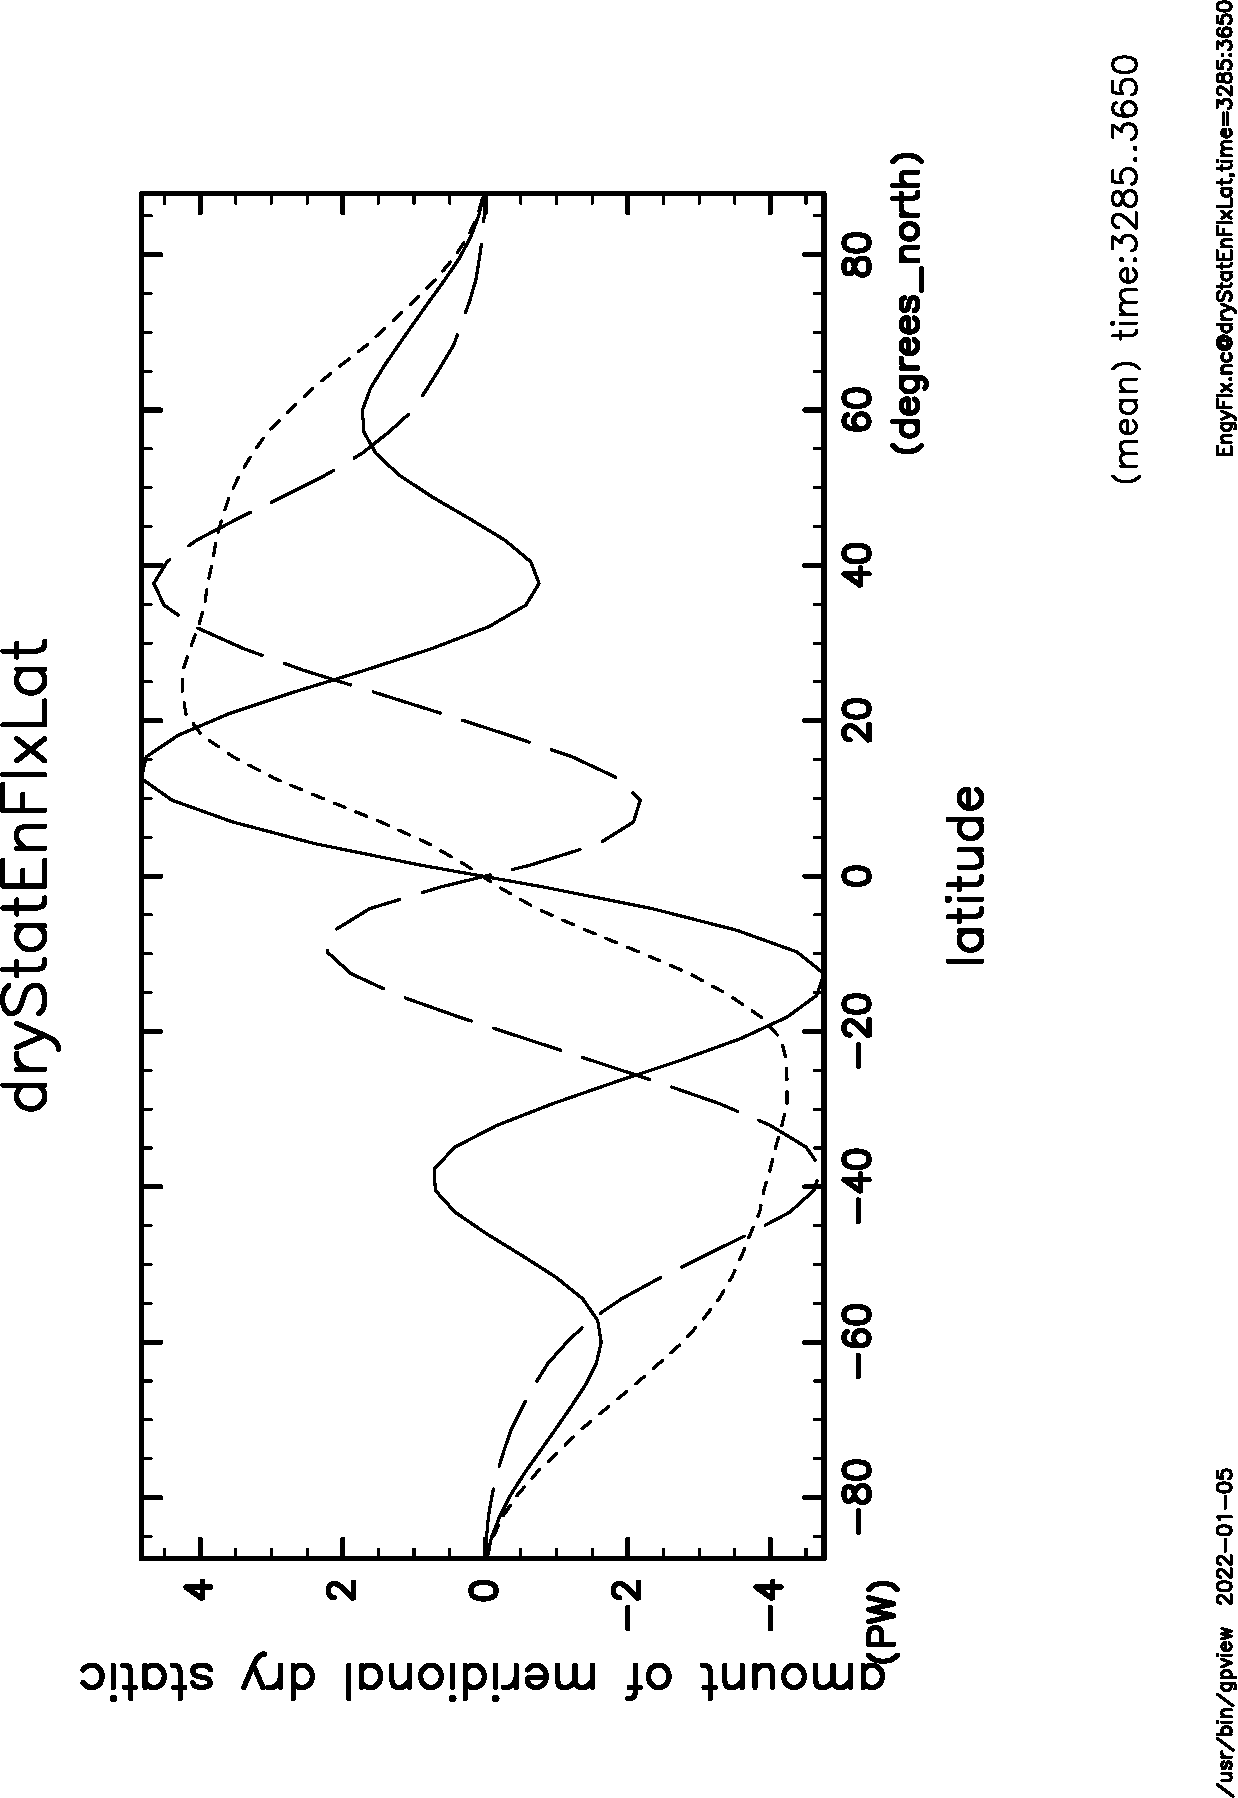
\includegraphics[height=\textwidth,angle=-90]{S1600/EngyFlx,time=3285:3650-crop.pdf}
			\(S=1600\hmu{W/m^2}\)\\
			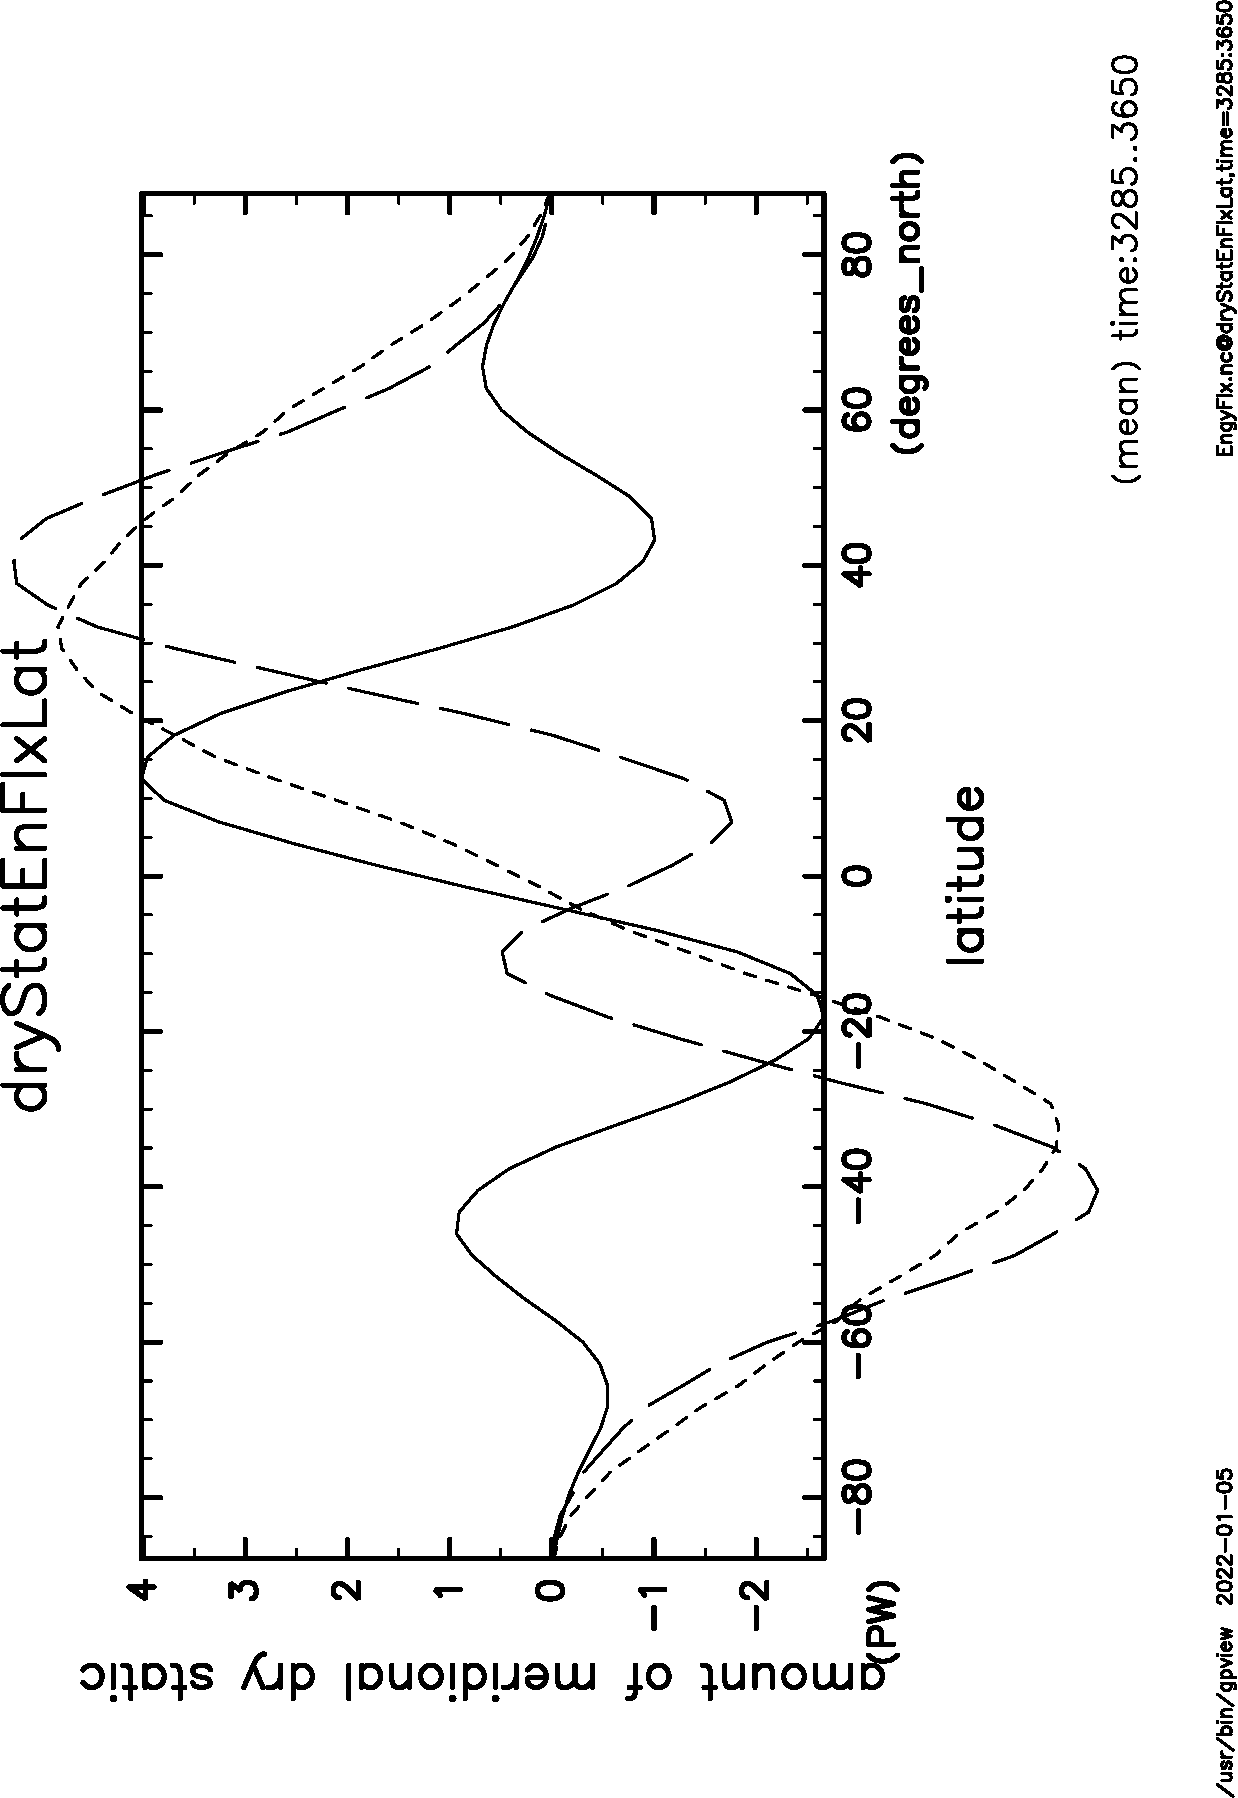
\includegraphics[height=\textwidth,angle=-90]{S1800/EngyFlx,time=3285:3650-crop.pdf}
			\(S=1800\hmu{W/m^2}\)
		\end{column}
		\begin{column}{.3\textwidth}
			\centering
			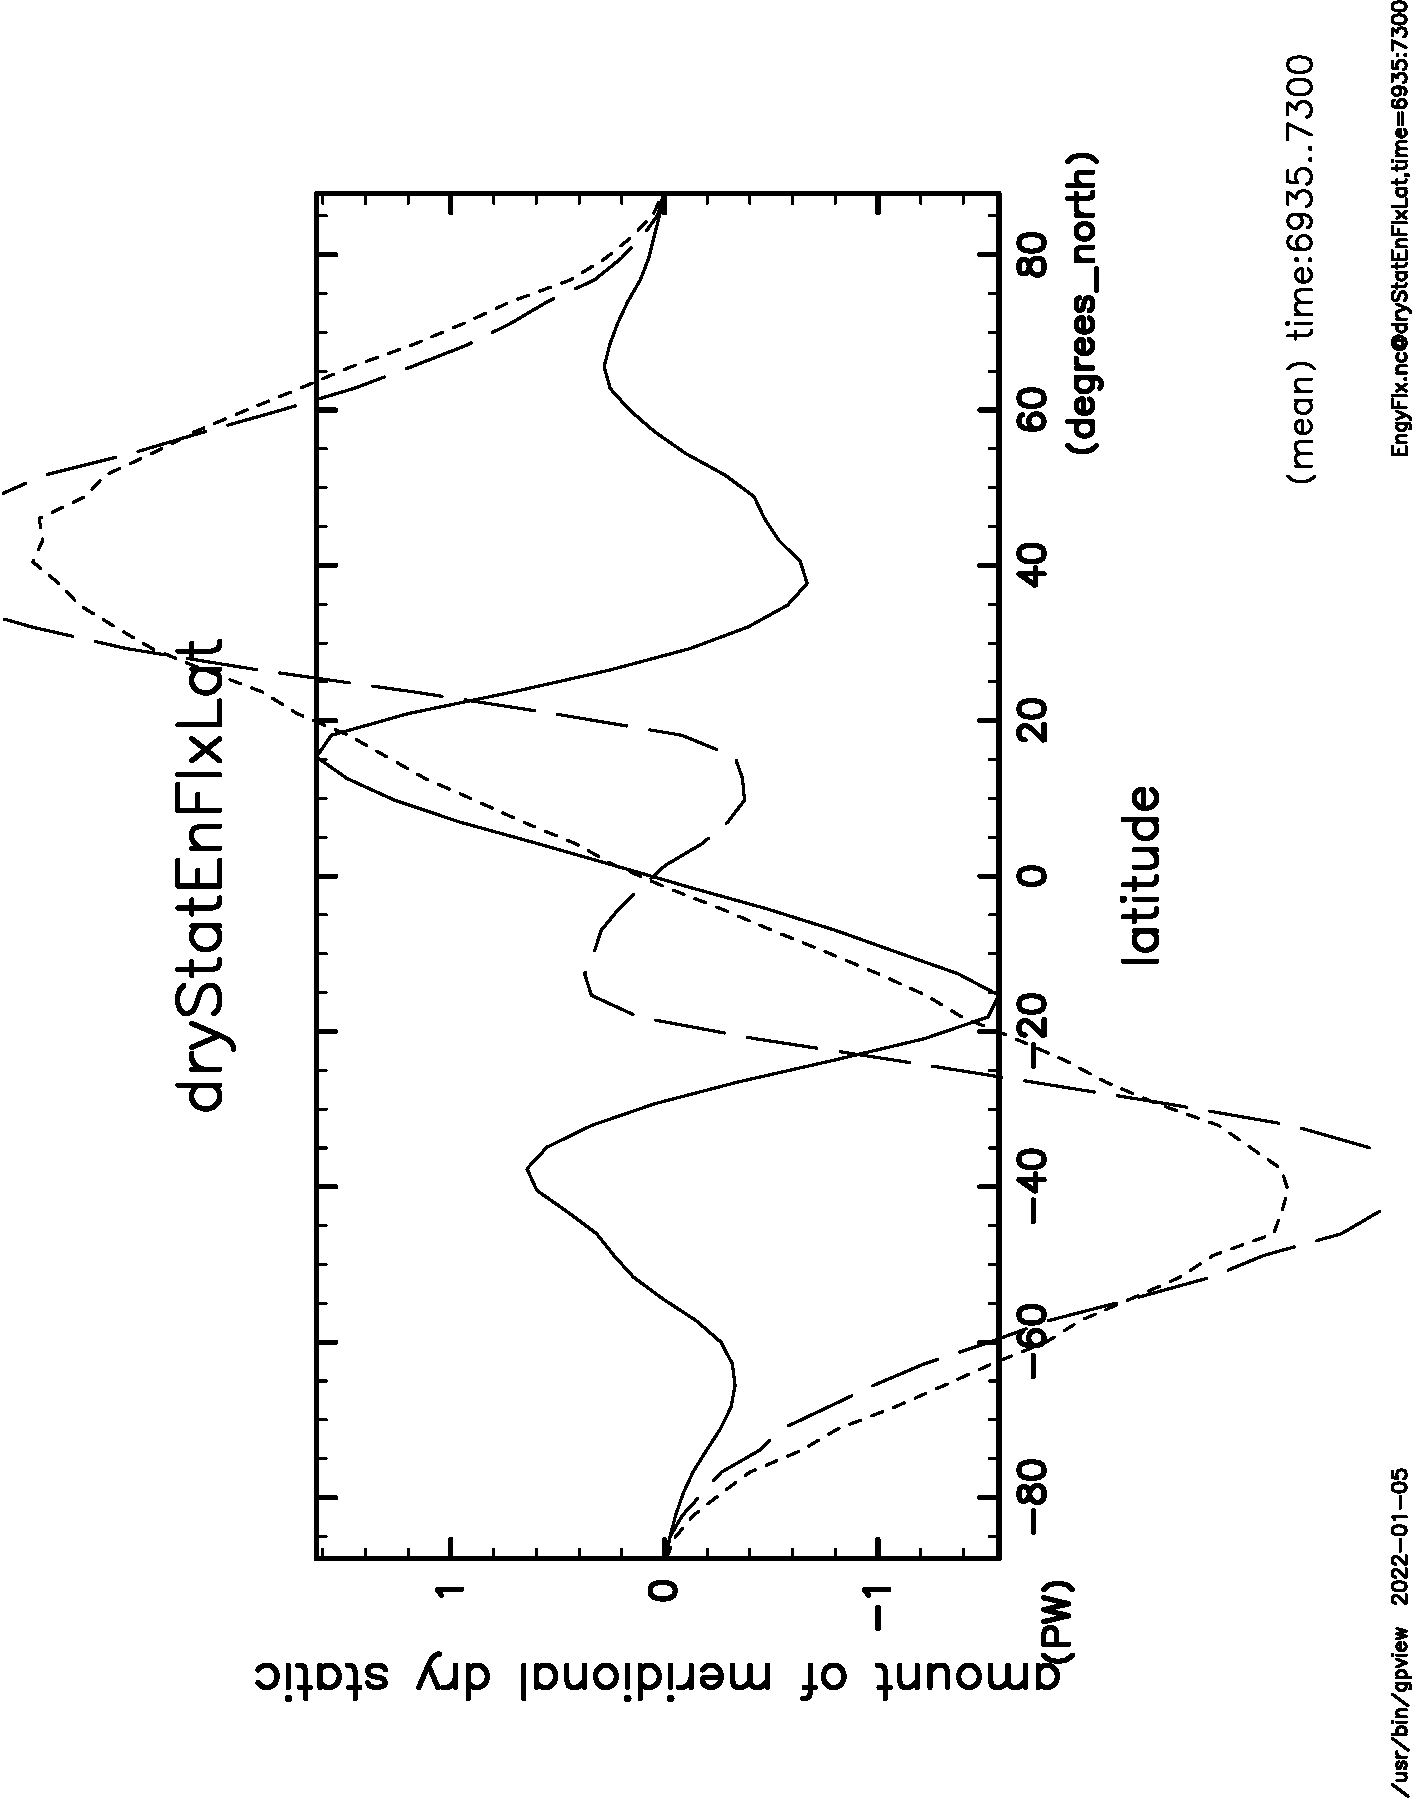
\includegraphics[height=\textwidth,angle=-90]{S2000/EngyFlx,time=6935:7300-crop.pdf}
			\(S=2000\hmu{W/m^2}\)
		\end{column}
	\end{columns}
	実線: dryStatEnFlxLat; 破線: latentEnFlxLat; 鎖線: moistStatFlxLat;
\end{frame}

\begin{frame}
	\frametitle{結果 (南北風; 計算終了年での平均)}
	\begin{columns}[T]
		\begin{column}{.3\textwidth}
			\centering
			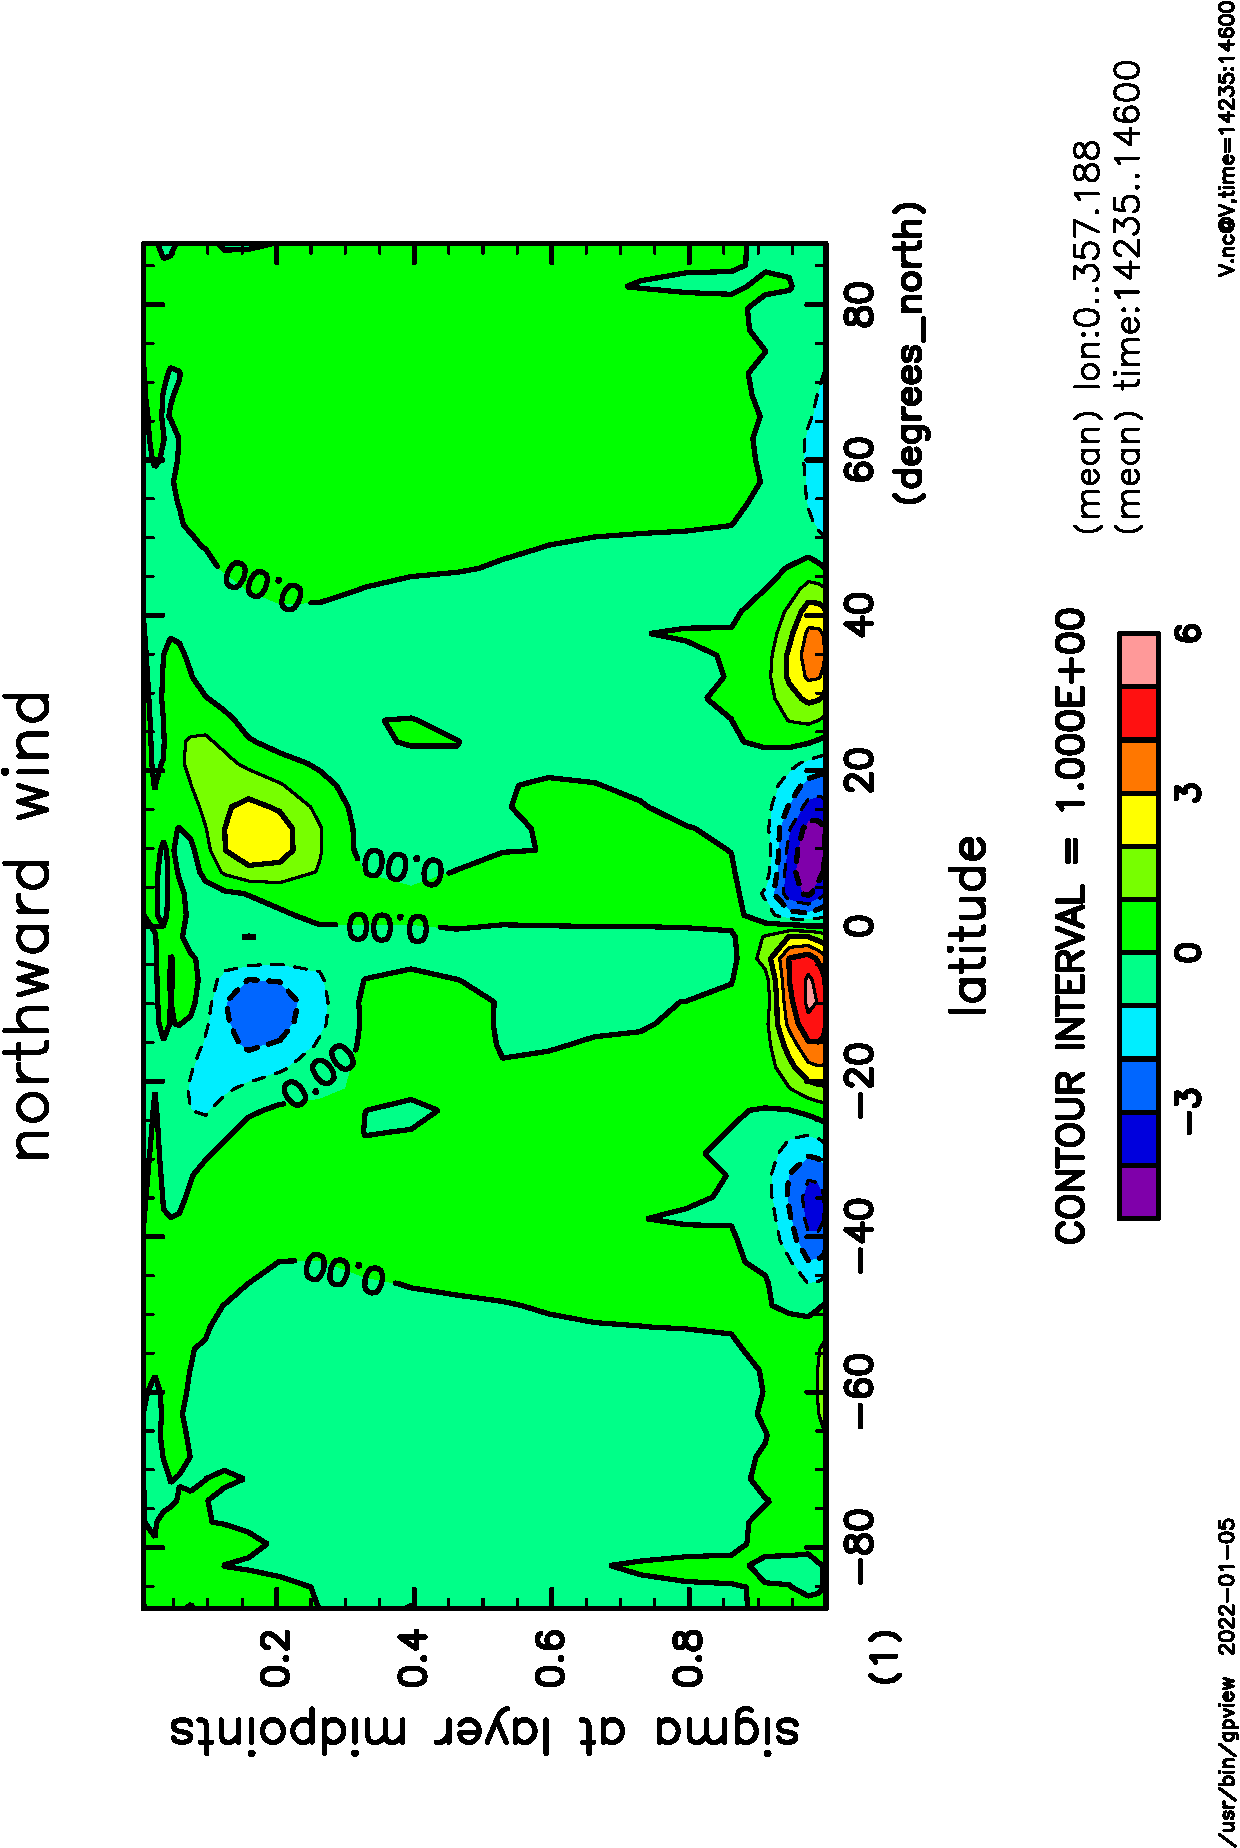
\includegraphics[height=\textwidth,angle=-90]{S1366/V,time=14235:14600-crop.pdf}
			\(S=1366\hmu{W/m^2}\)\\
			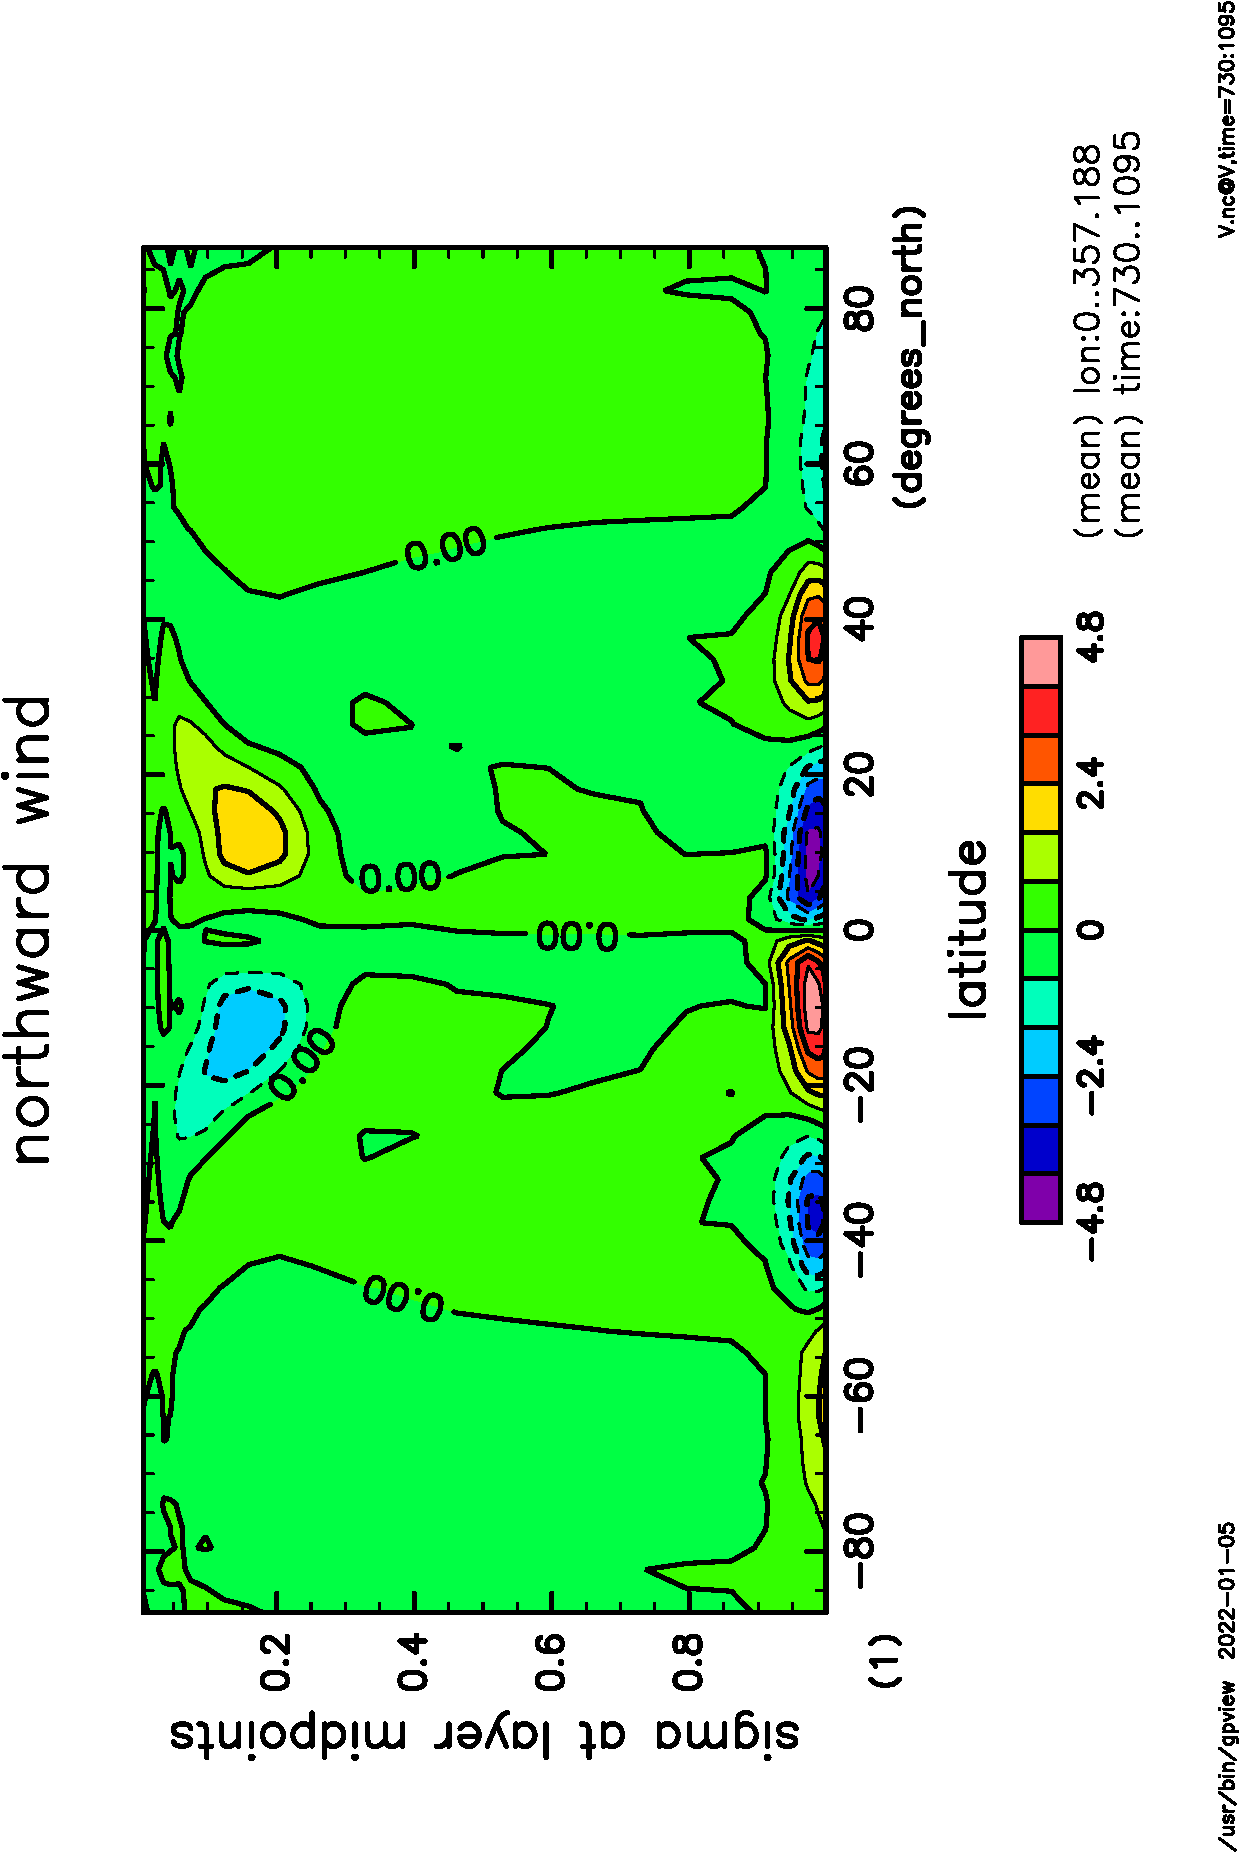
\includegraphics[height=\textwidth,angle=-90]{S1500/V,time=730:1095-crop.pdf}
			\(S=1500\hmu{W/m^2}\)
		\end{column}
		\begin{column}{.3\textwidth}
			\centering
			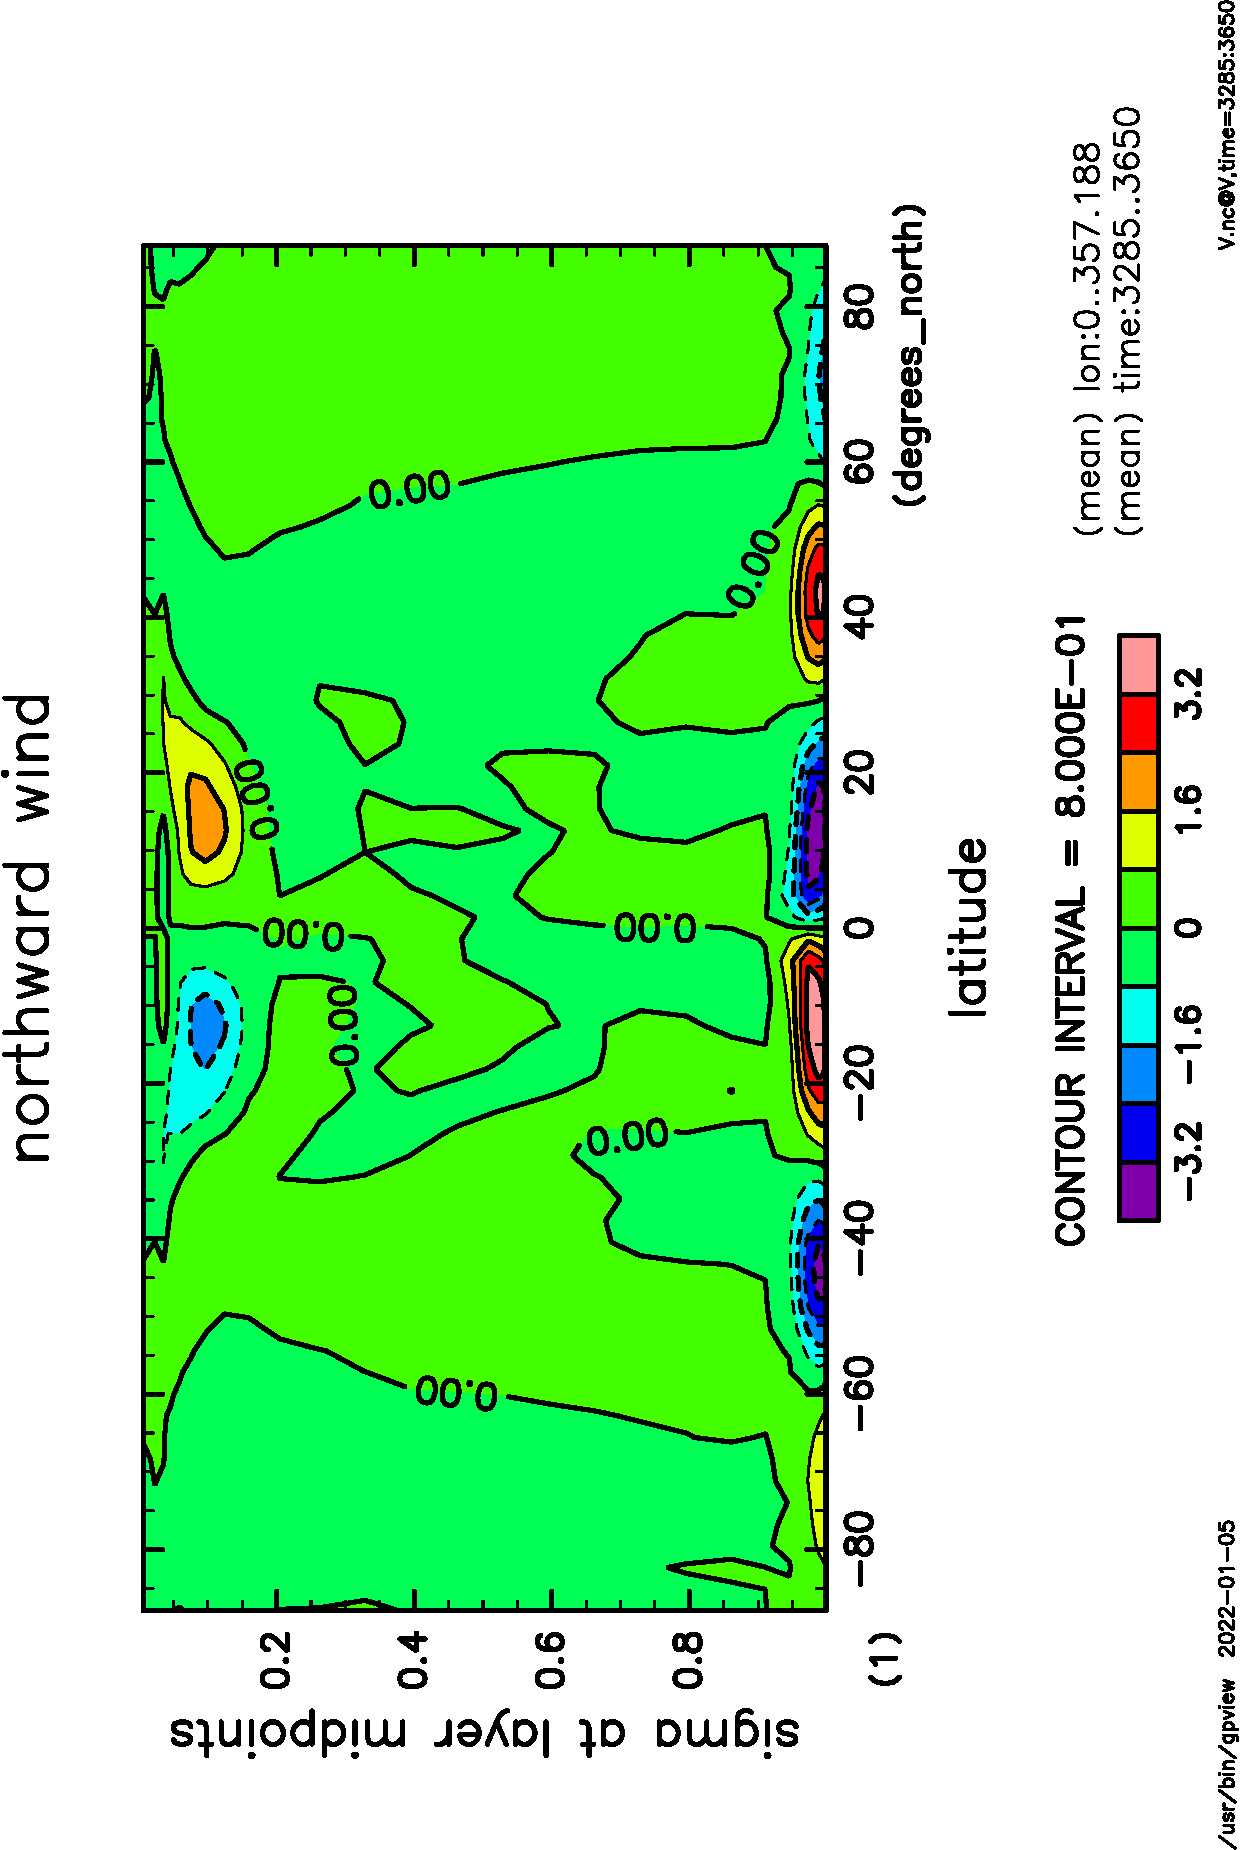
\includegraphics[height=\textwidth,angle=-90]{S1600/V,time=3285:3650-crop.pdf}
			\(S=1600\hmu{W/m^2}\)\\
			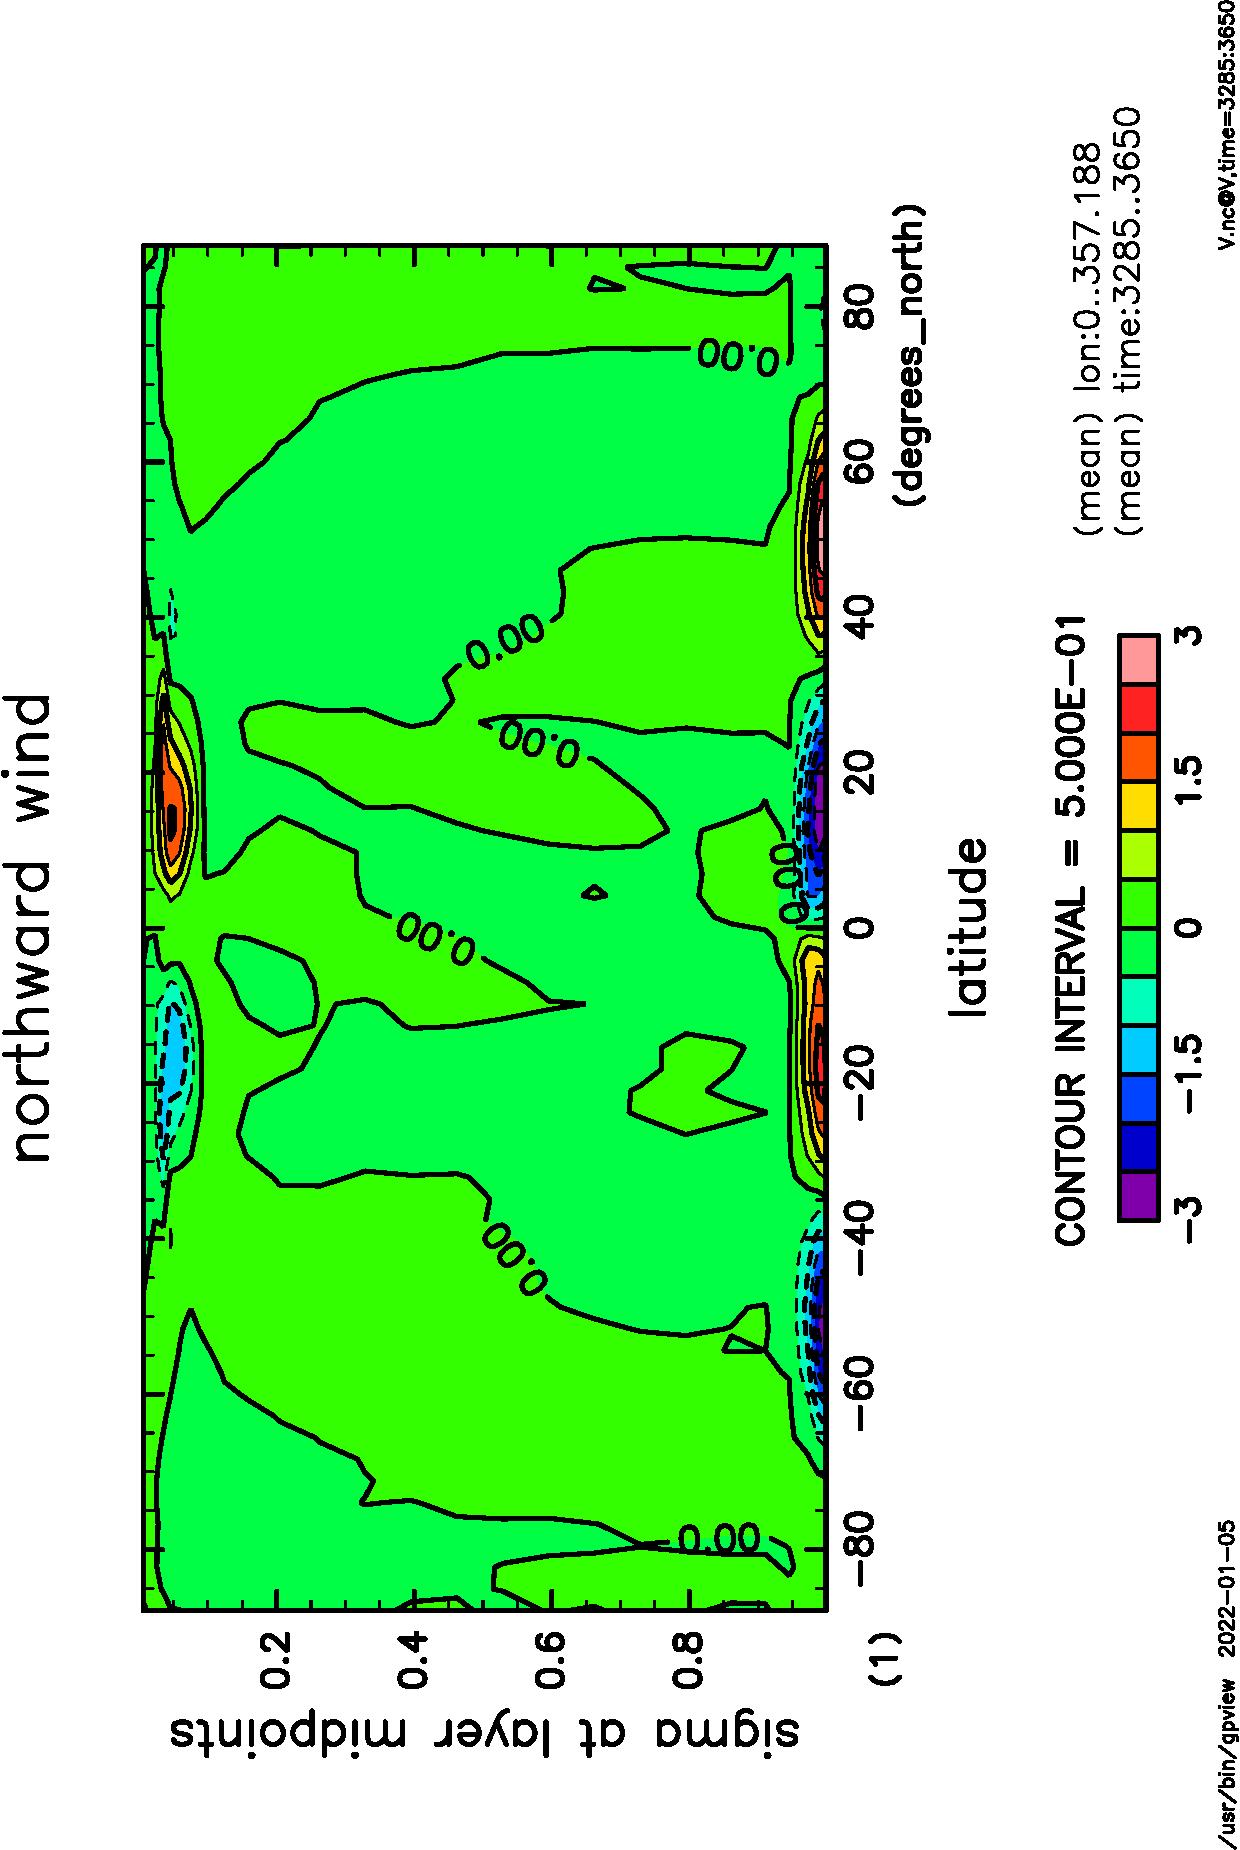
\includegraphics[height=\textwidth,angle=-90]{S1800/V,time=3285:3650-crop.pdf}
			\(S=1800\hmu{W/m^2}\)
		\end{column}
		\begin{column}{.3\textwidth}
			\centering
			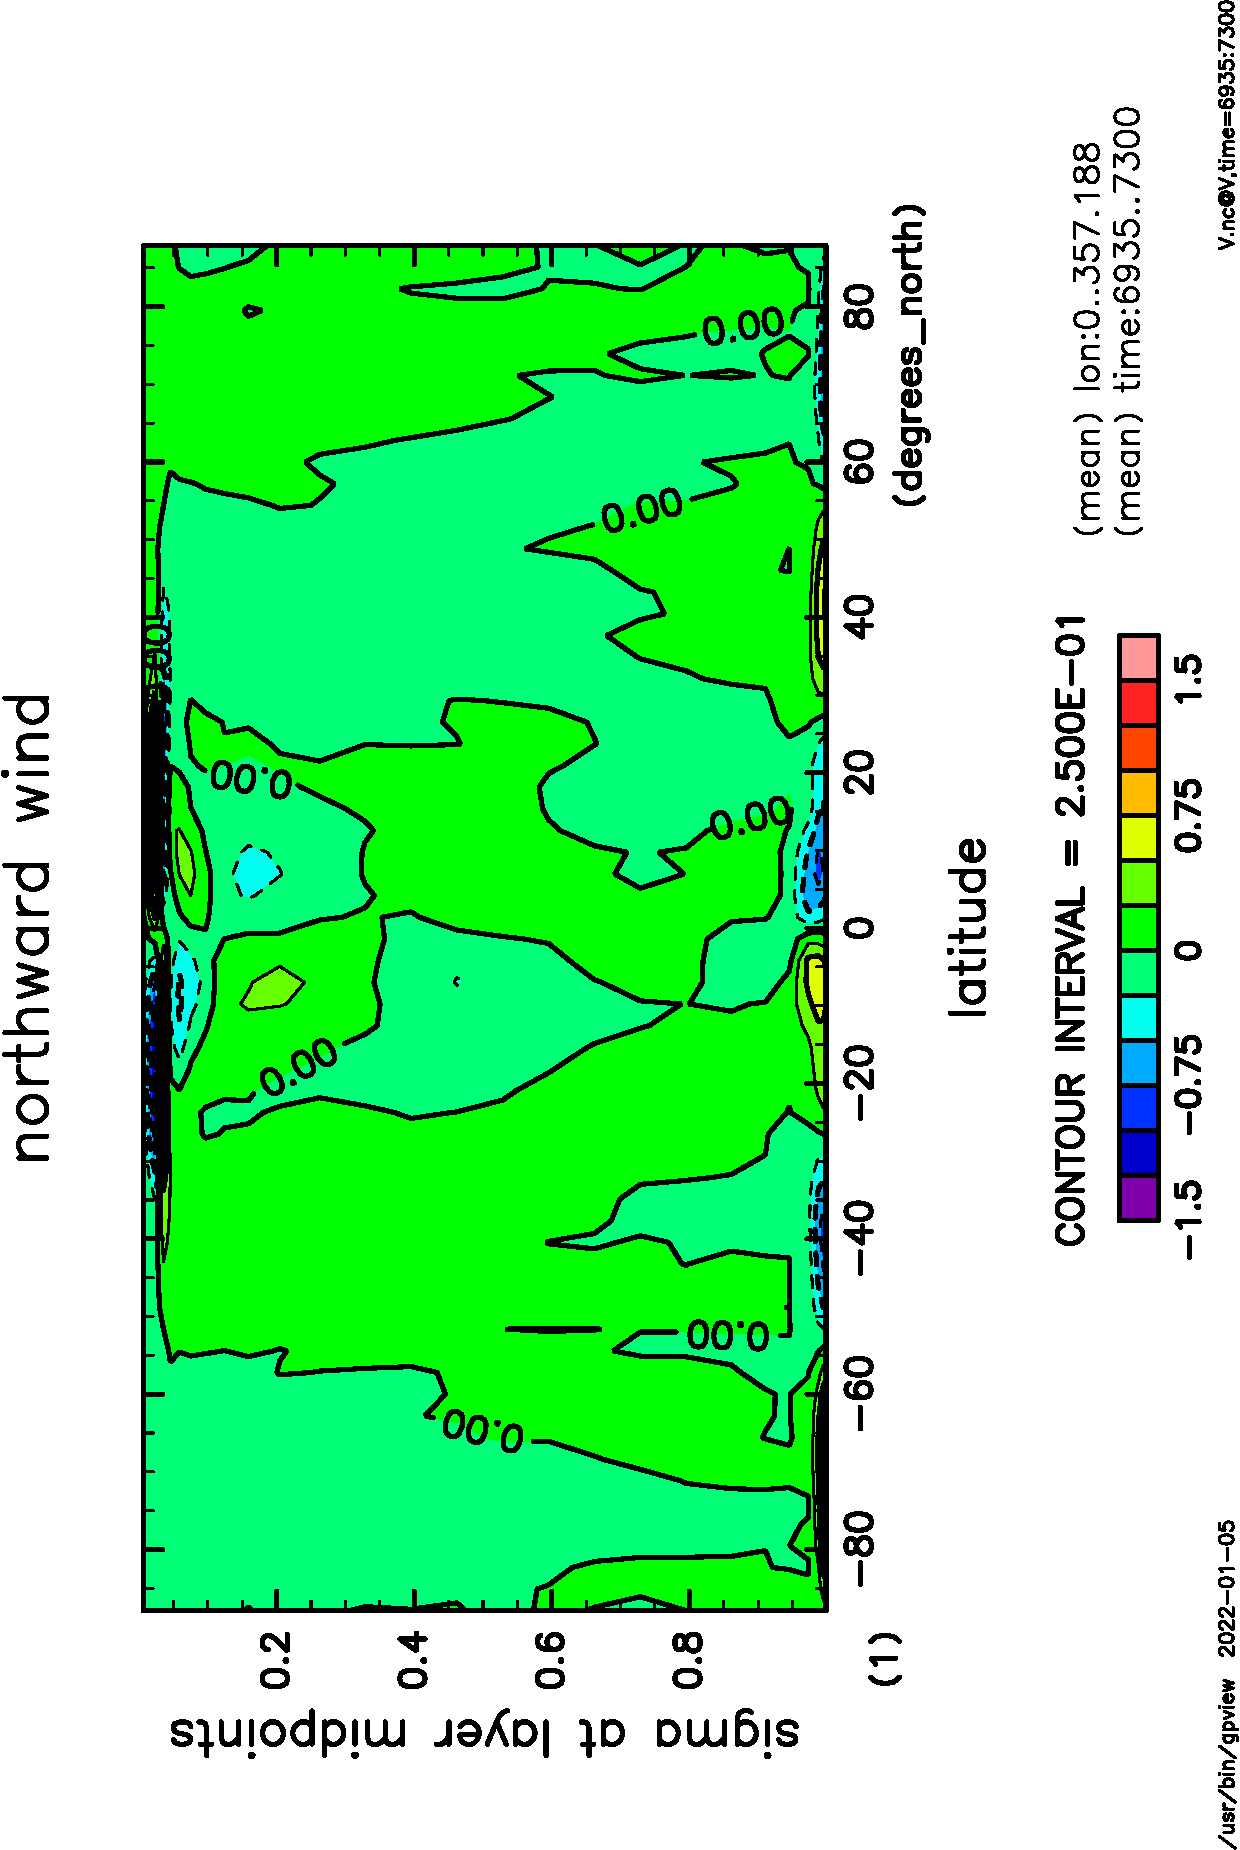
\includegraphics[height=\textwidth,angle=-90]{S2000/V,time=6935:7300-crop.pdf}
			\(S=2000\hmu{W/m^2}\)
		\end{column}
	\end{columns}
\end{frame}

\begin{frame}
	\frametitle{結果 (比湿; 計算終了年での平均)}
	\begin{columns}[T]
		\begin{column}{.3\textwidth}
			\centering
			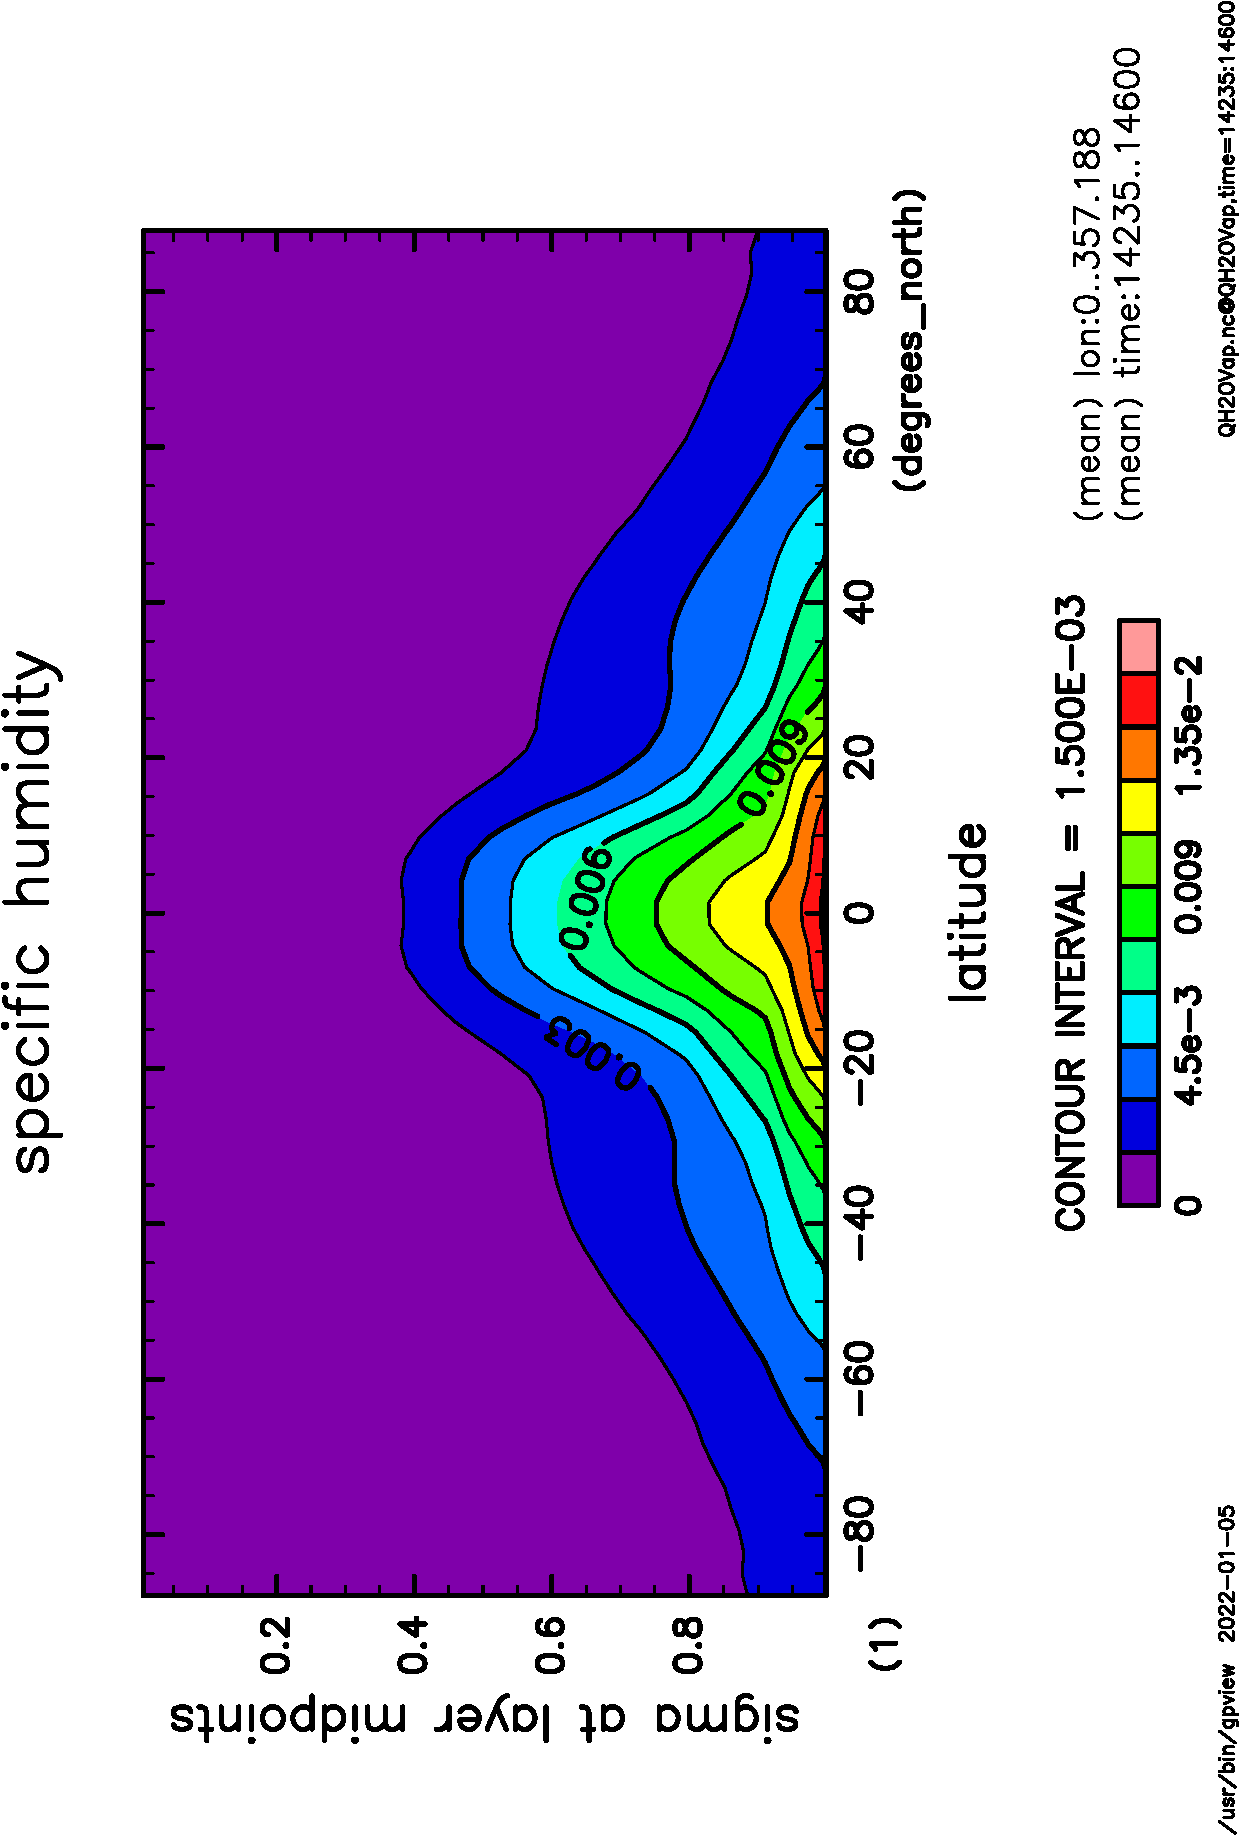
\includegraphics[height=\textwidth,angle=-90]{S1366/QH2OVap,time=14235:14600-crop.pdf}
			\(S=1366\hmu{W/m^2}\)\\
			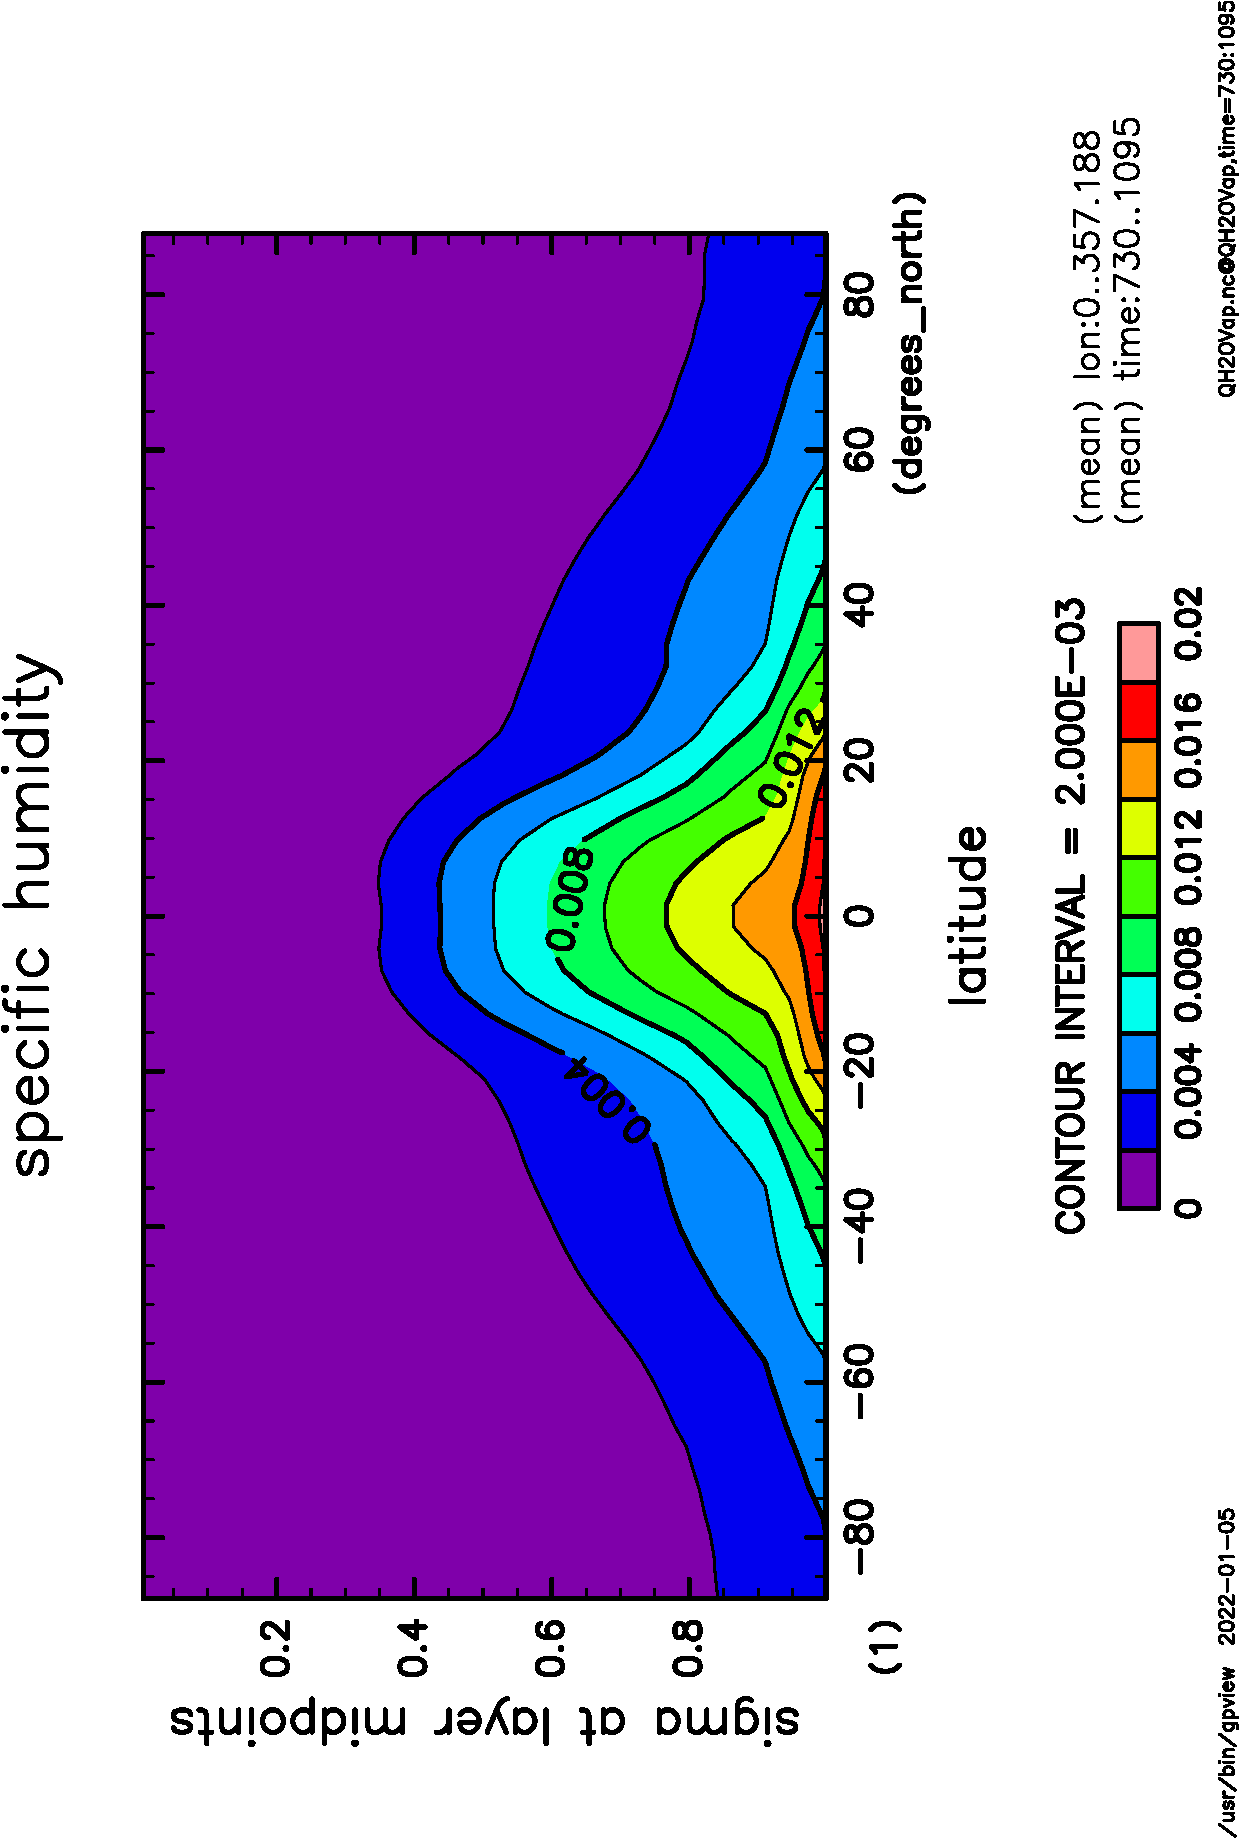
\includegraphics[height=\textwidth,angle=-90]{S1500/QH2OVap,time=730:1095-crop.pdf}
			\(S=1500\hmu{W/m^2}\)
		\end{column}
		\begin{column}{.3\textwidth}
			\centering
			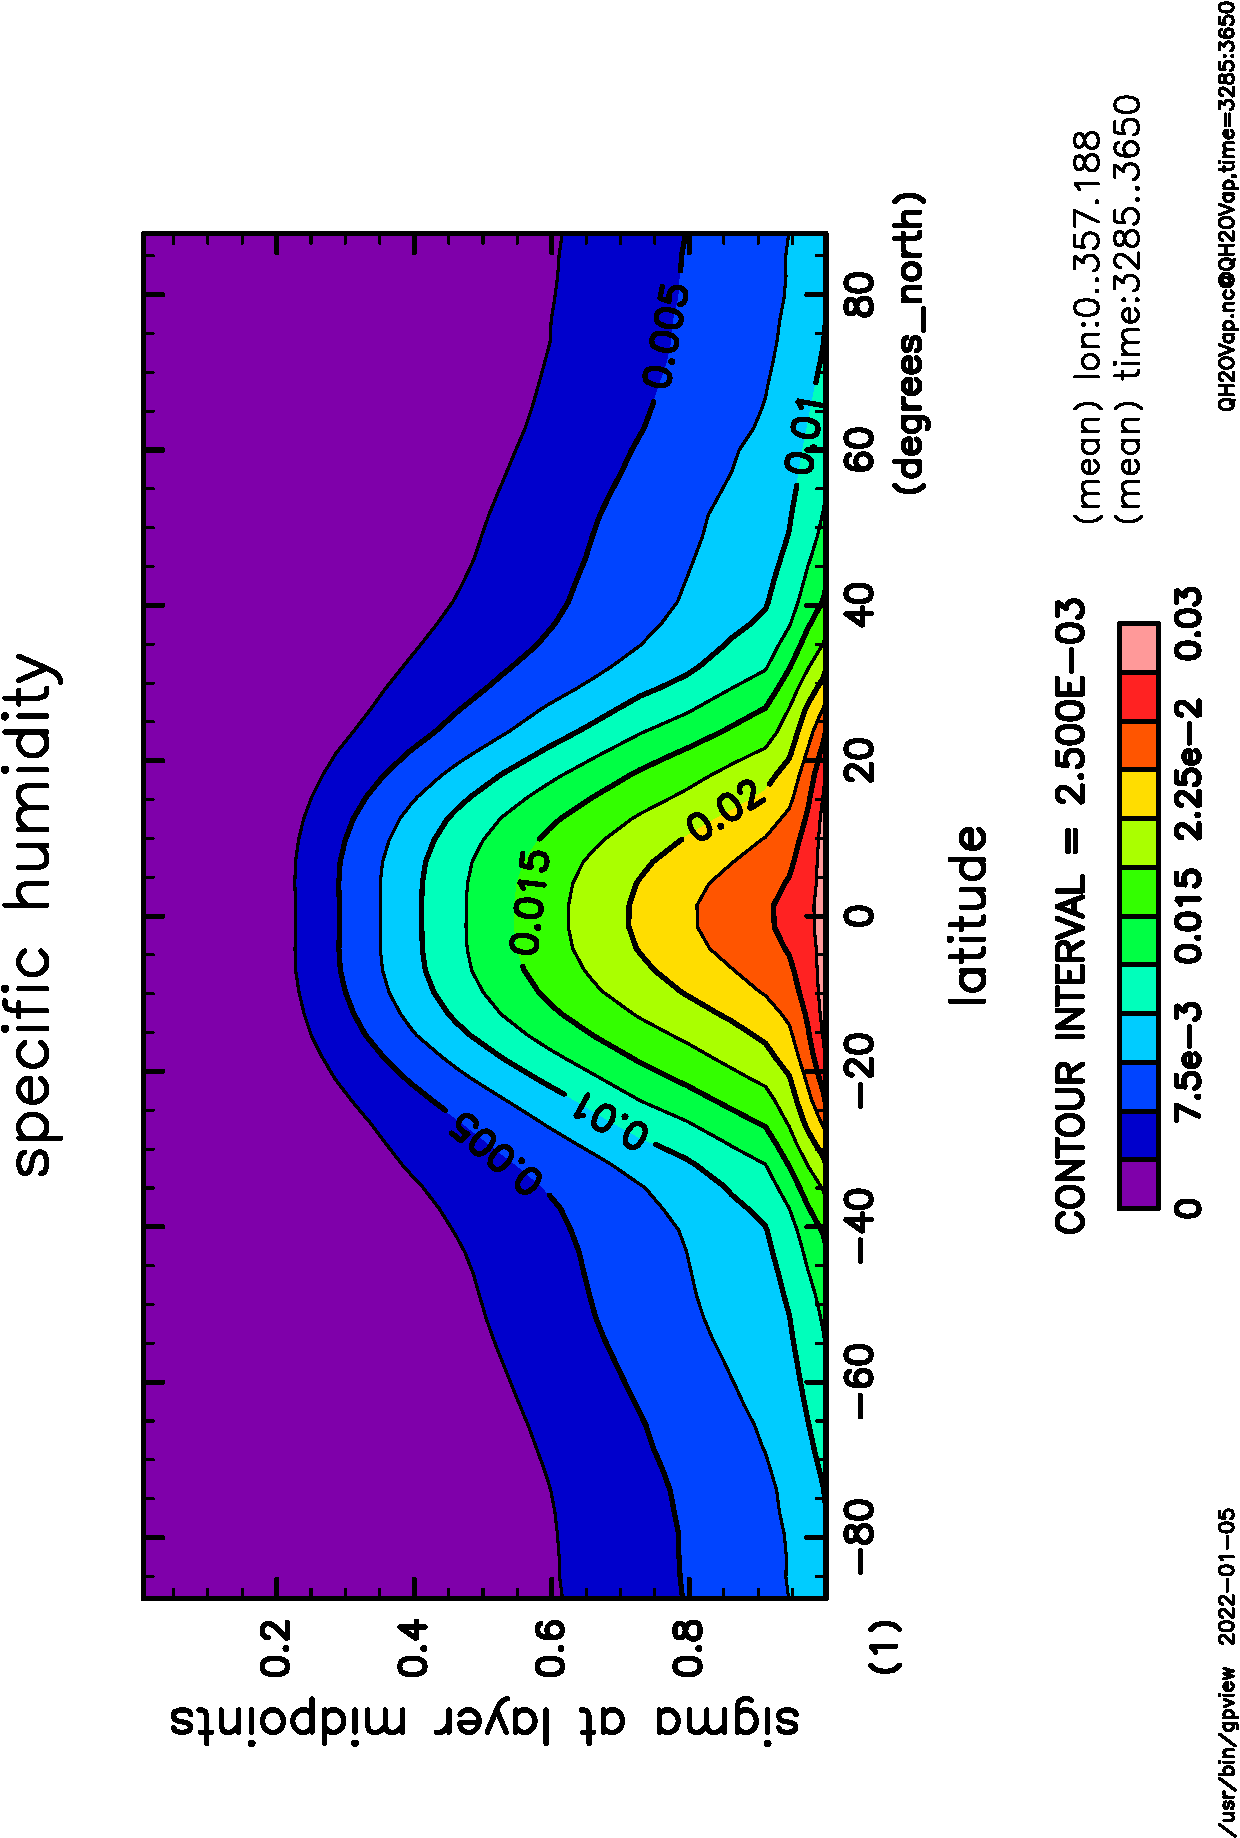
\includegraphics[height=\textwidth,angle=-90]{S1600/QH2OVap,time=3285:3650-crop.pdf}
			\(S=1600\hmu{W/m^2}\)\\
			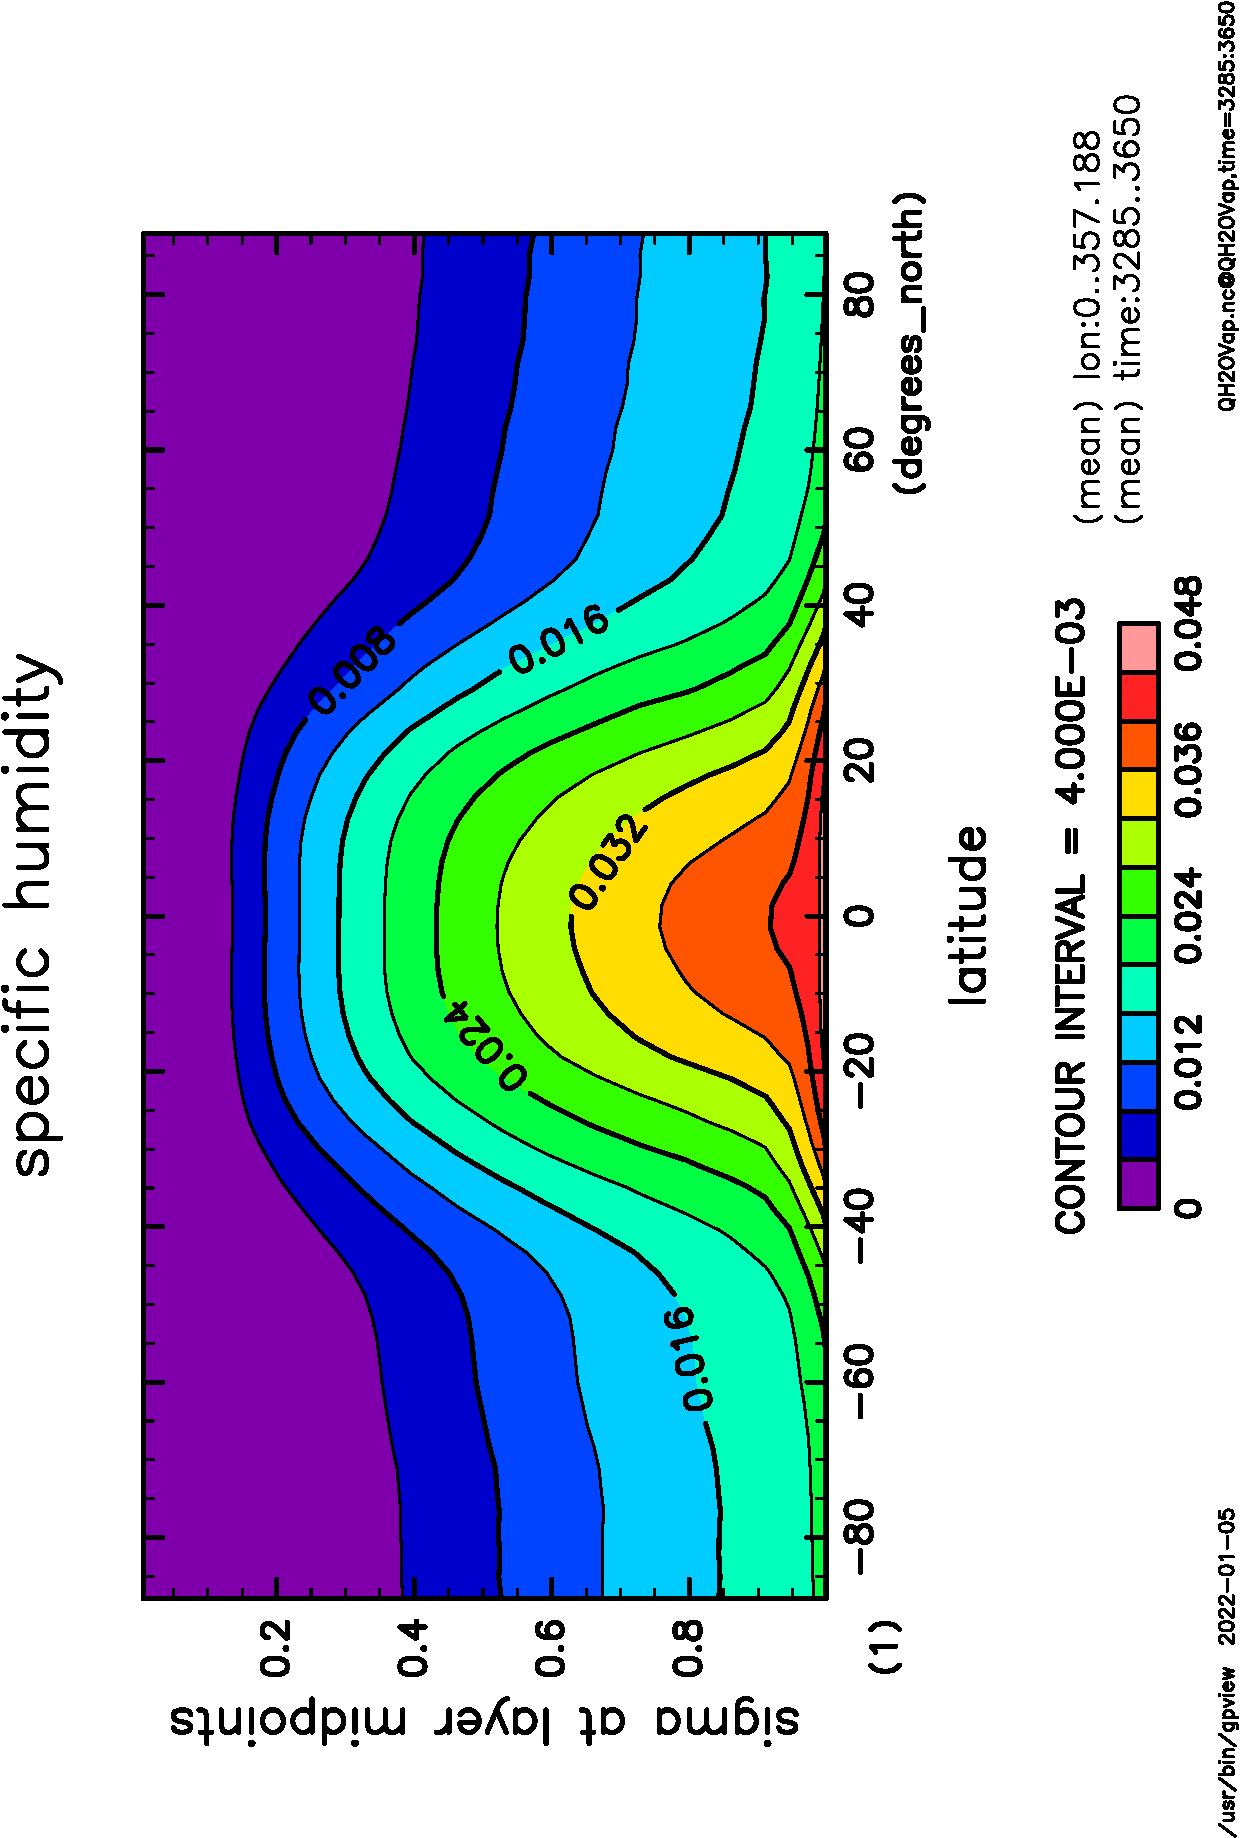
\includegraphics[height=\textwidth,angle=-90]{S1800/QH2OVap,time=3285:3650-crop.pdf}
			\(S=1800\hmu{W/m^2}\)
		\end{column}
		\begin{column}{.3\textwidth}
			\centering
			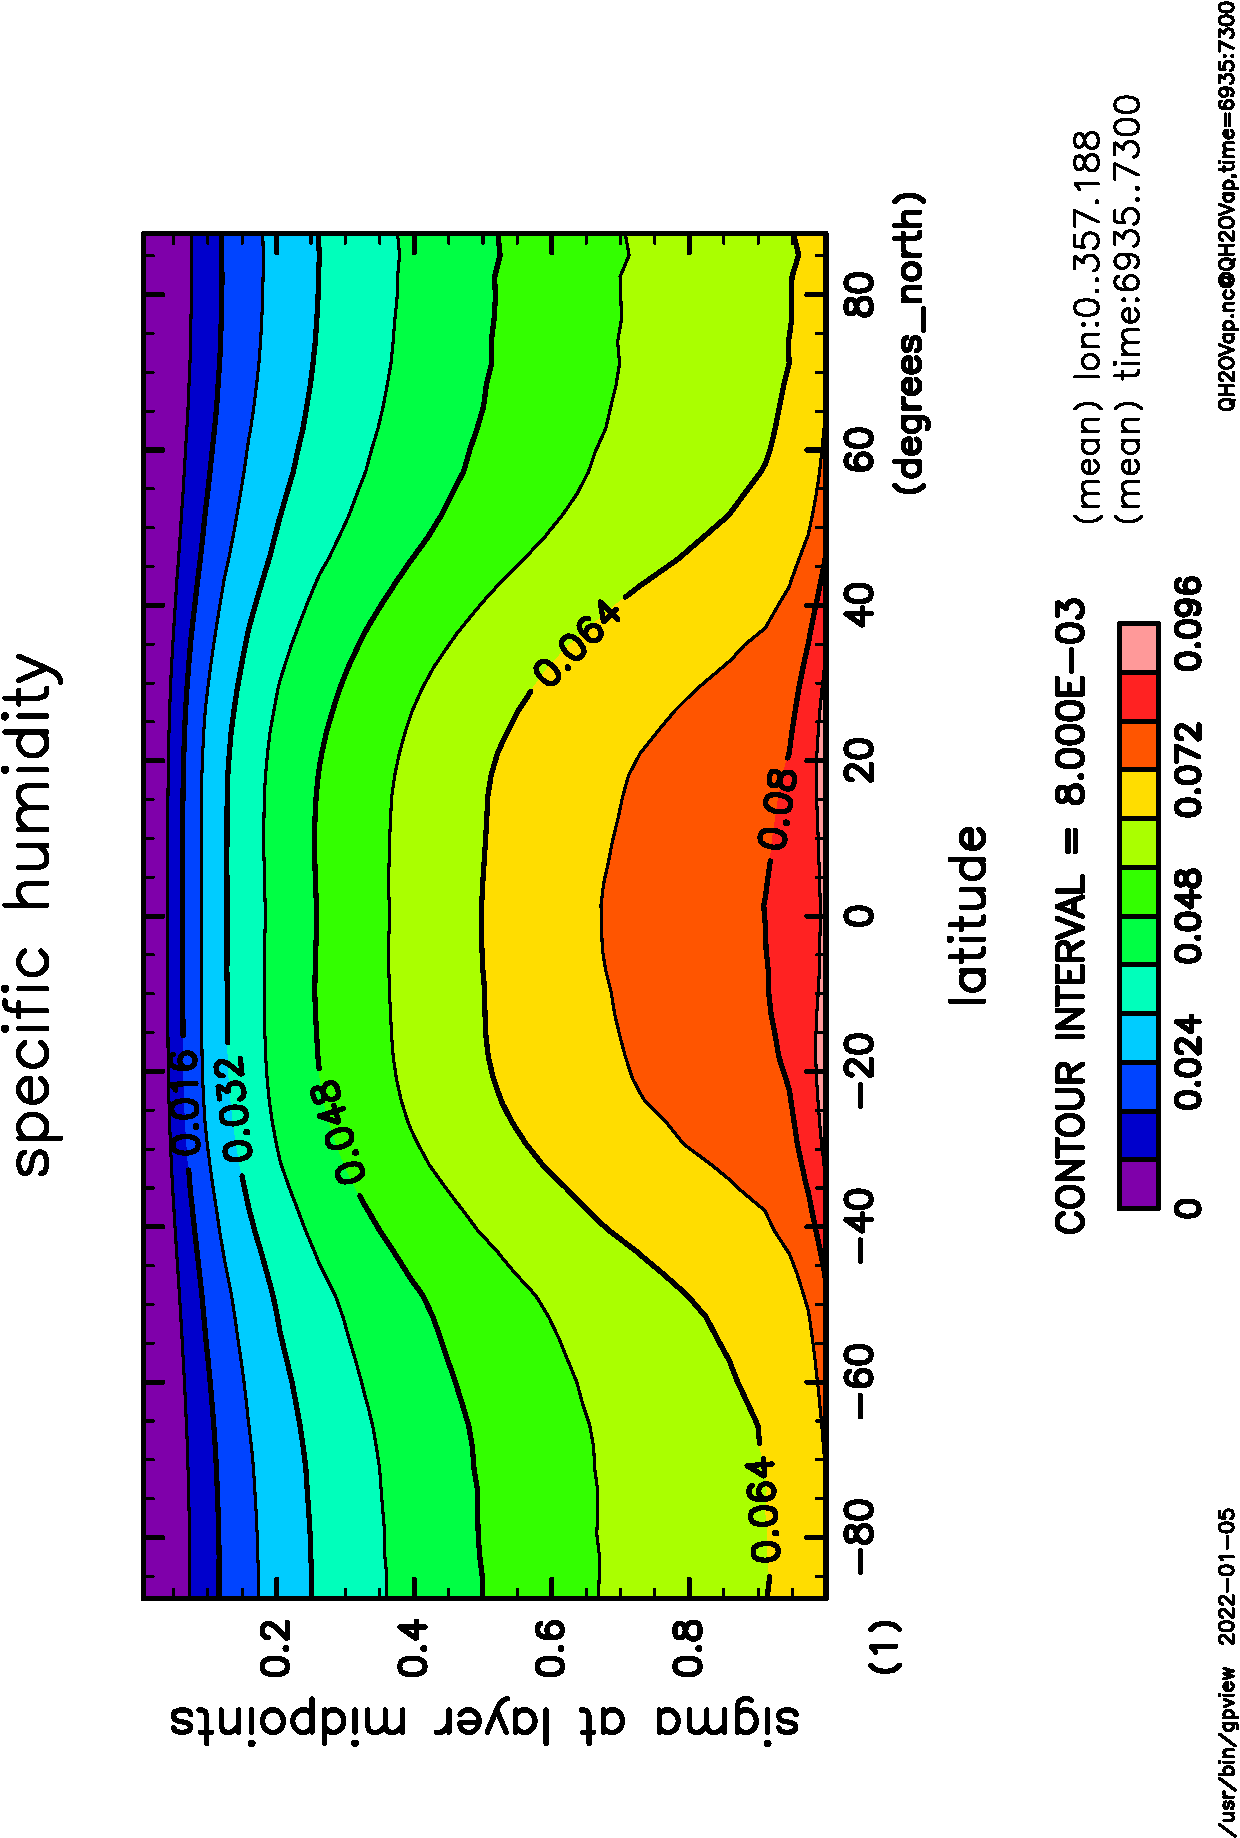
\includegraphics[height=\textwidth,angle=-90]{S2000/QH2OVap,time=6935:7300-crop.pdf}
			\(S=2000\hmu{W/m^2}\)
		\end{column}
	\end{columns}
\end{frame}

\begin{frame}
	\frametitle{結果 (気温; 計算終了年での平均)}
	\begin{columns}[T]
		\begin{column}{.3\textwidth}
			\centering
			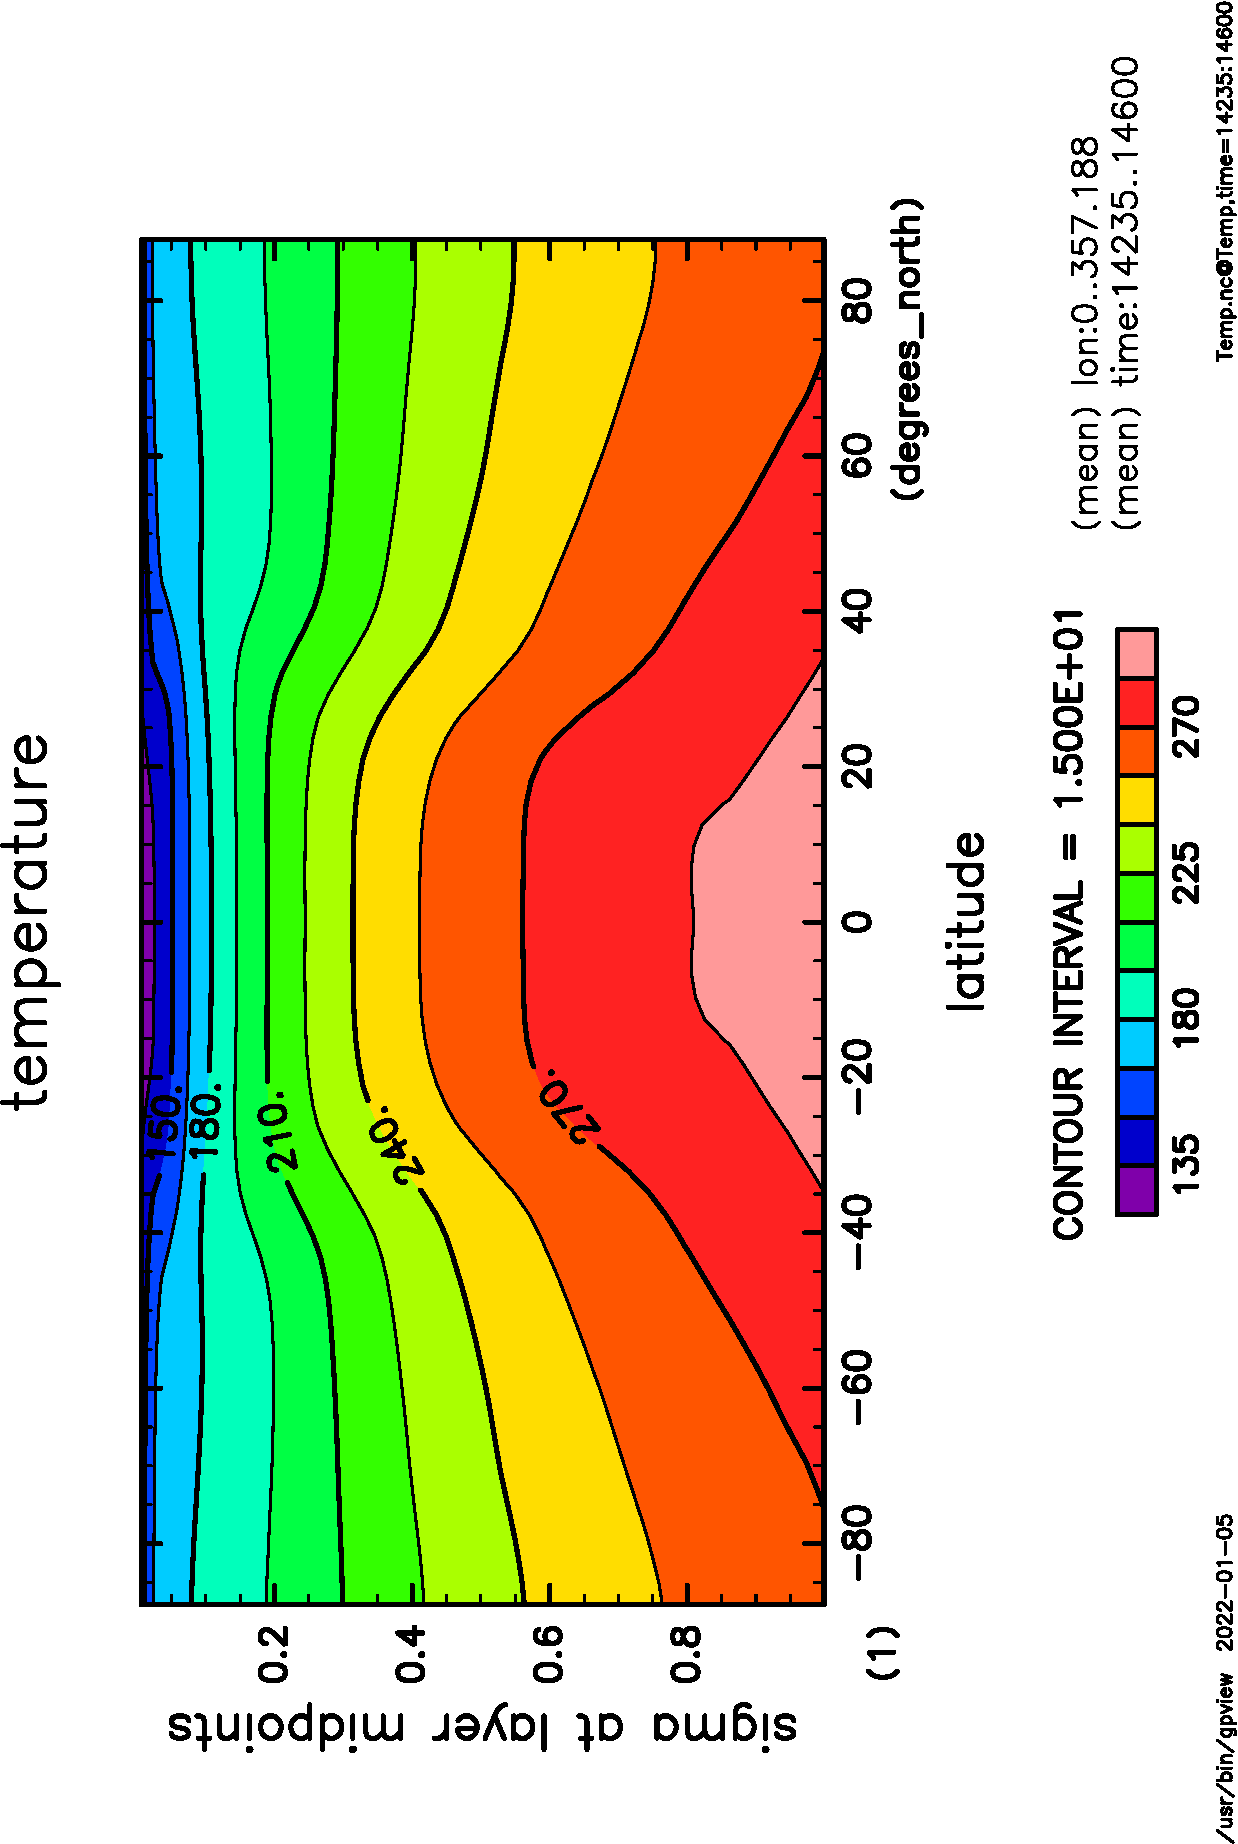
\includegraphics[height=\textwidth,angle=-90]{S1366/Temp,time=14235:14600-crop.pdf}
			\(S=1366\hmu{W/m^2}\)\\
			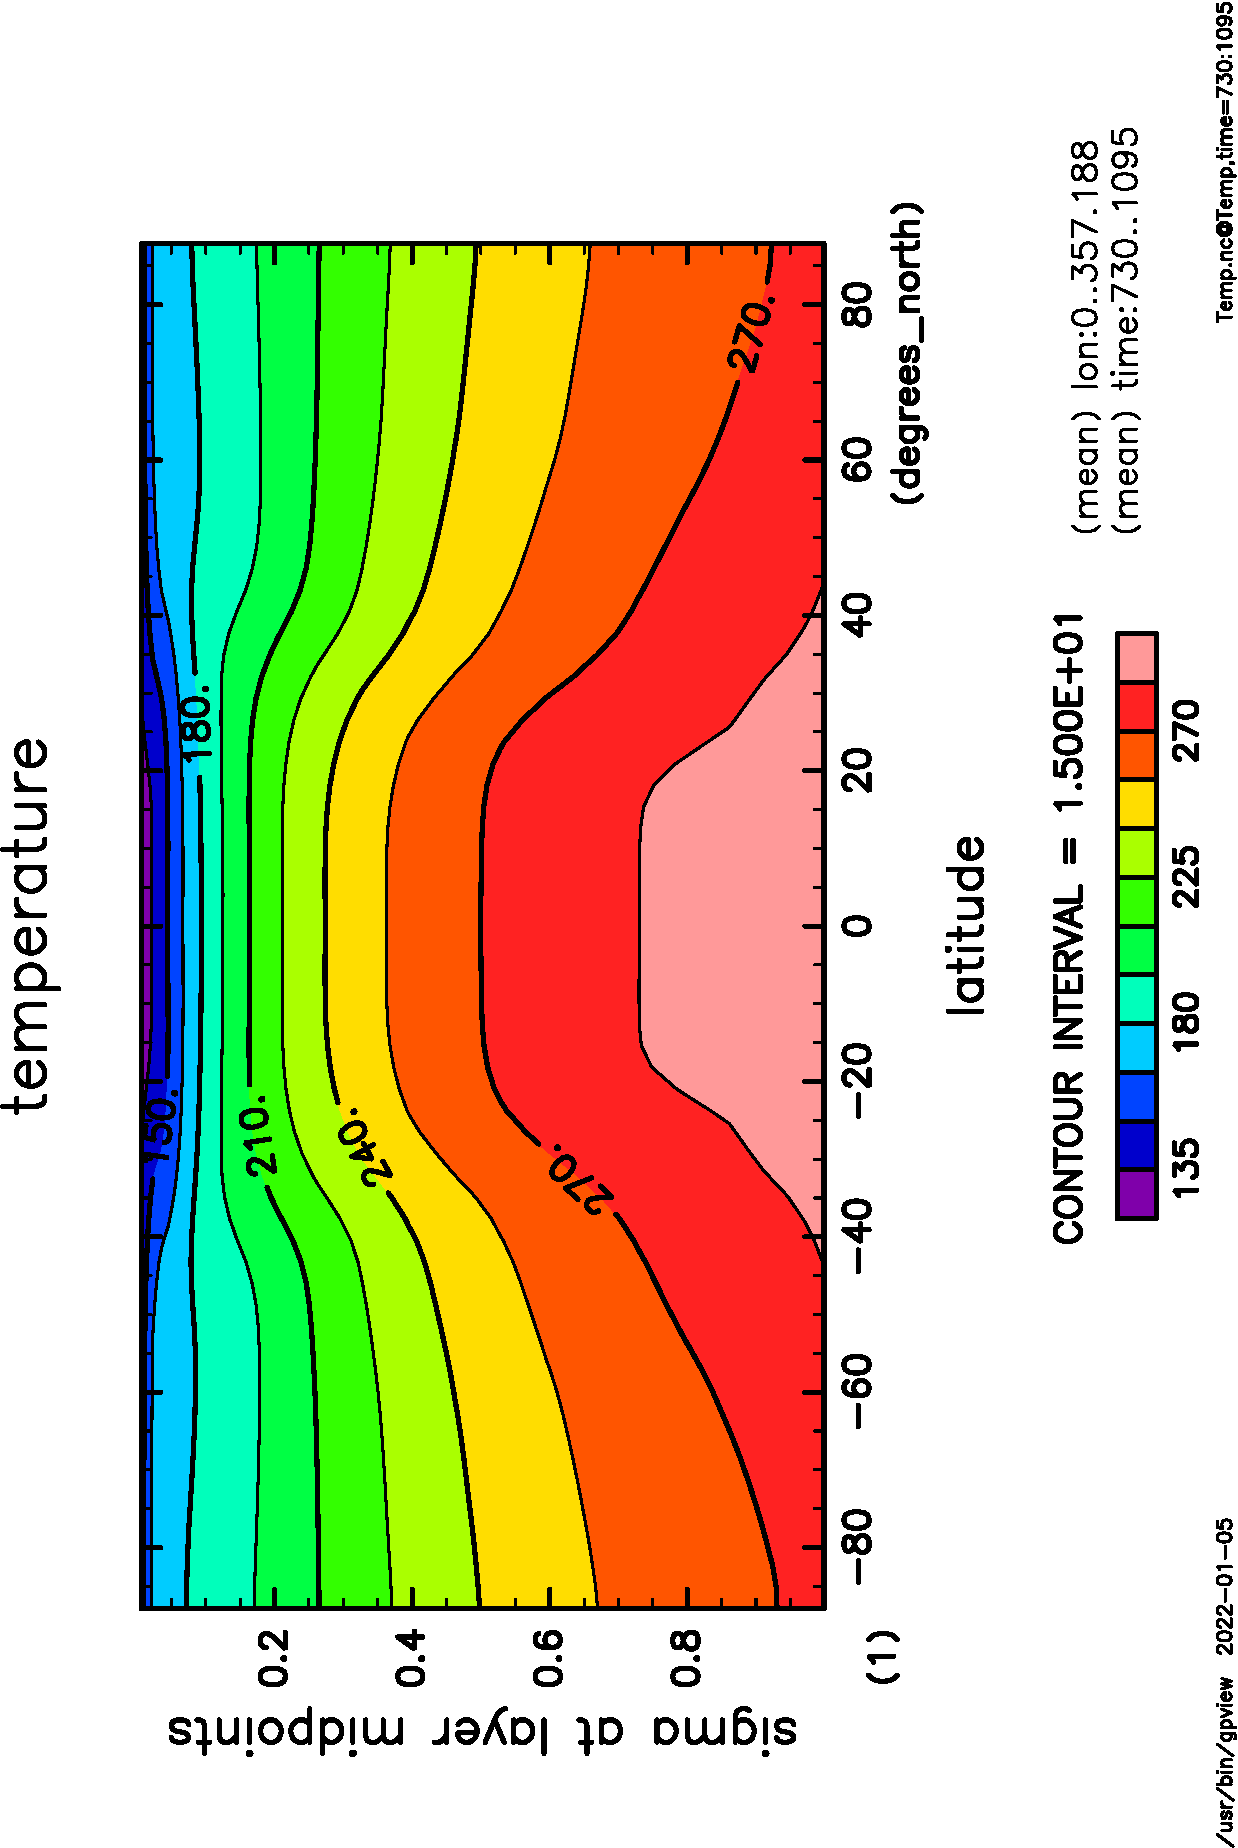
\includegraphics[height=\textwidth,angle=-90]{S1500/Temp,time=730:1095-crop.pdf}
			\(S=1500\hmu{W/m^2}\)
		\end{column}
		\begin{column}{.3\textwidth}
			\centering
			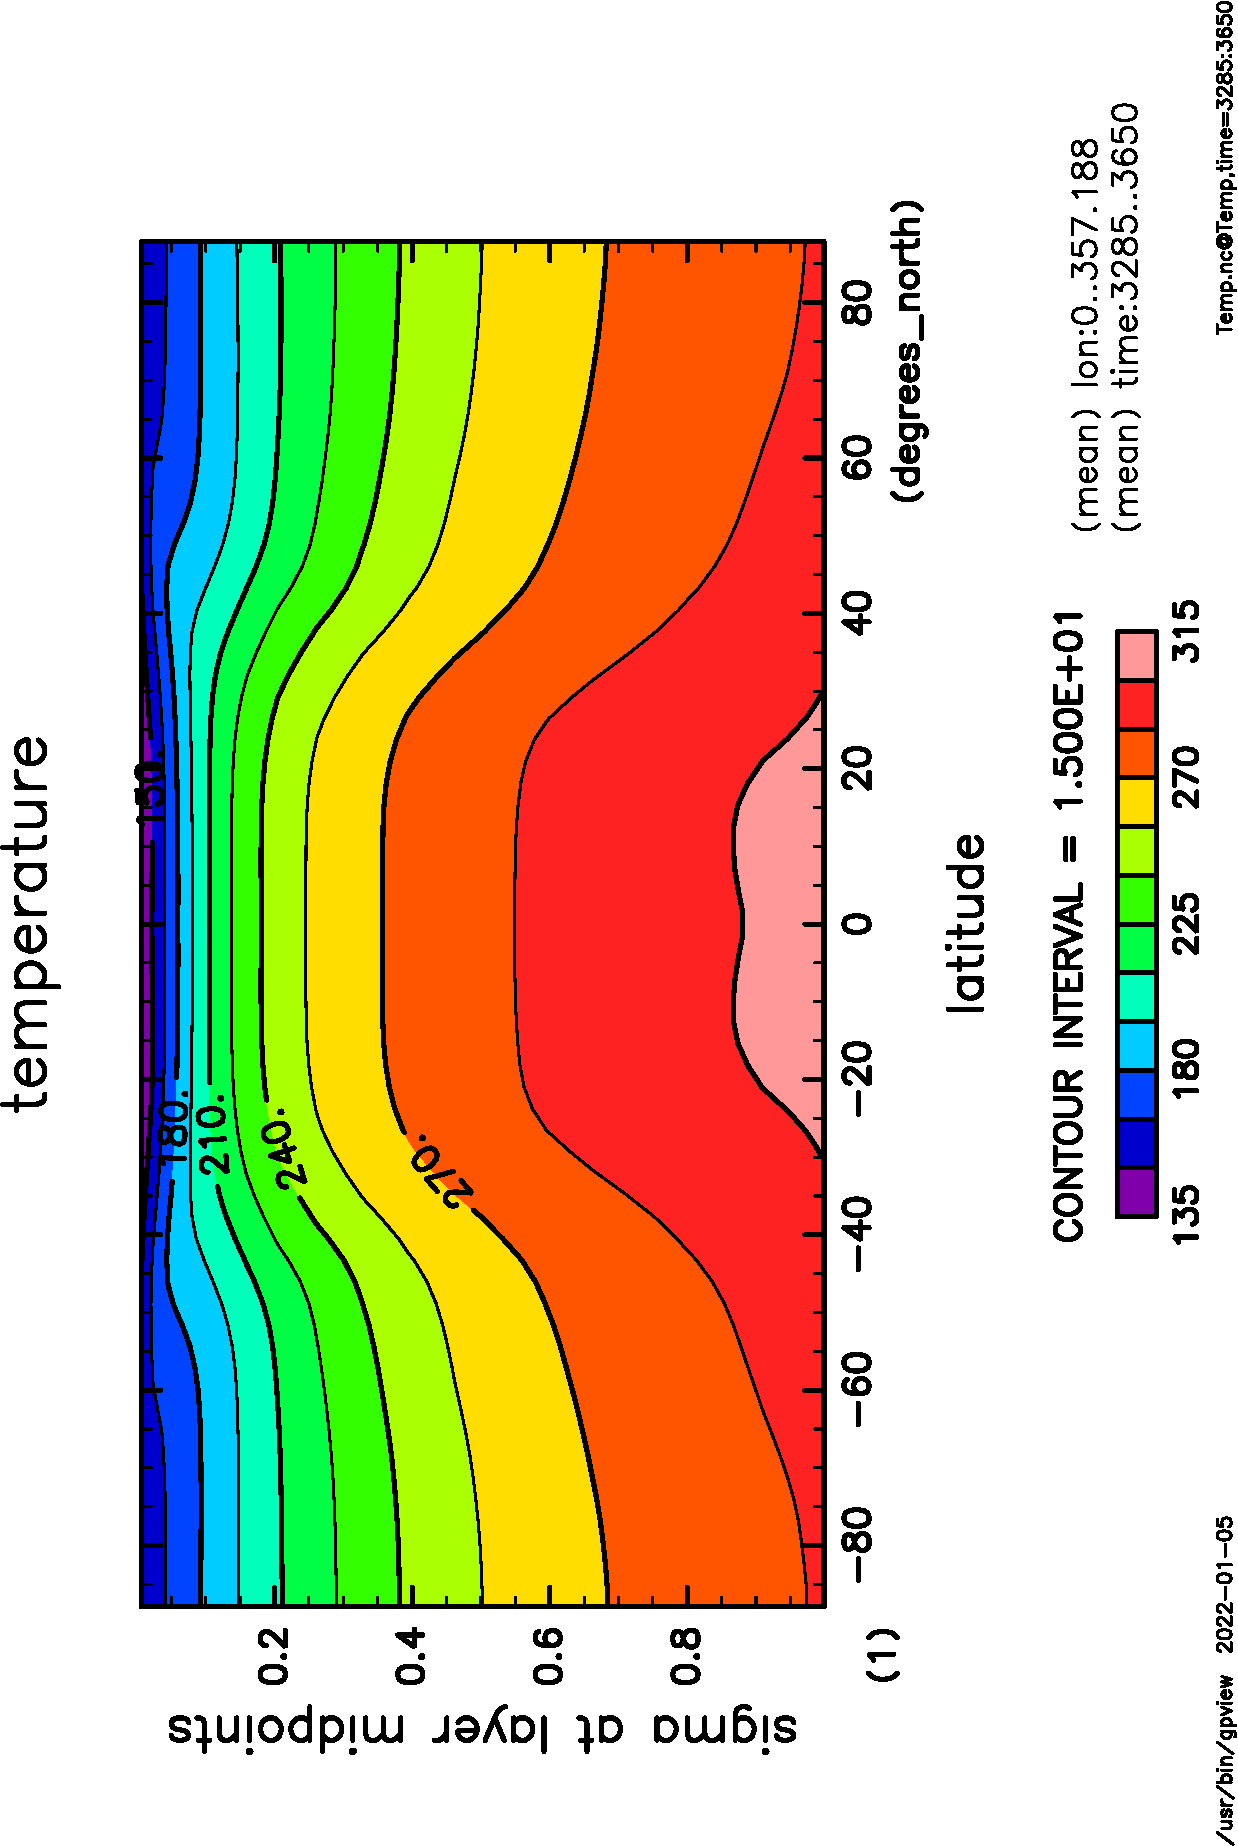
\includegraphics[height=\textwidth,angle=-90]{S1600/Temp,time=3285:3650-crop.pdf}
			\(S=1600\hmu{W/m^2}\)\\
			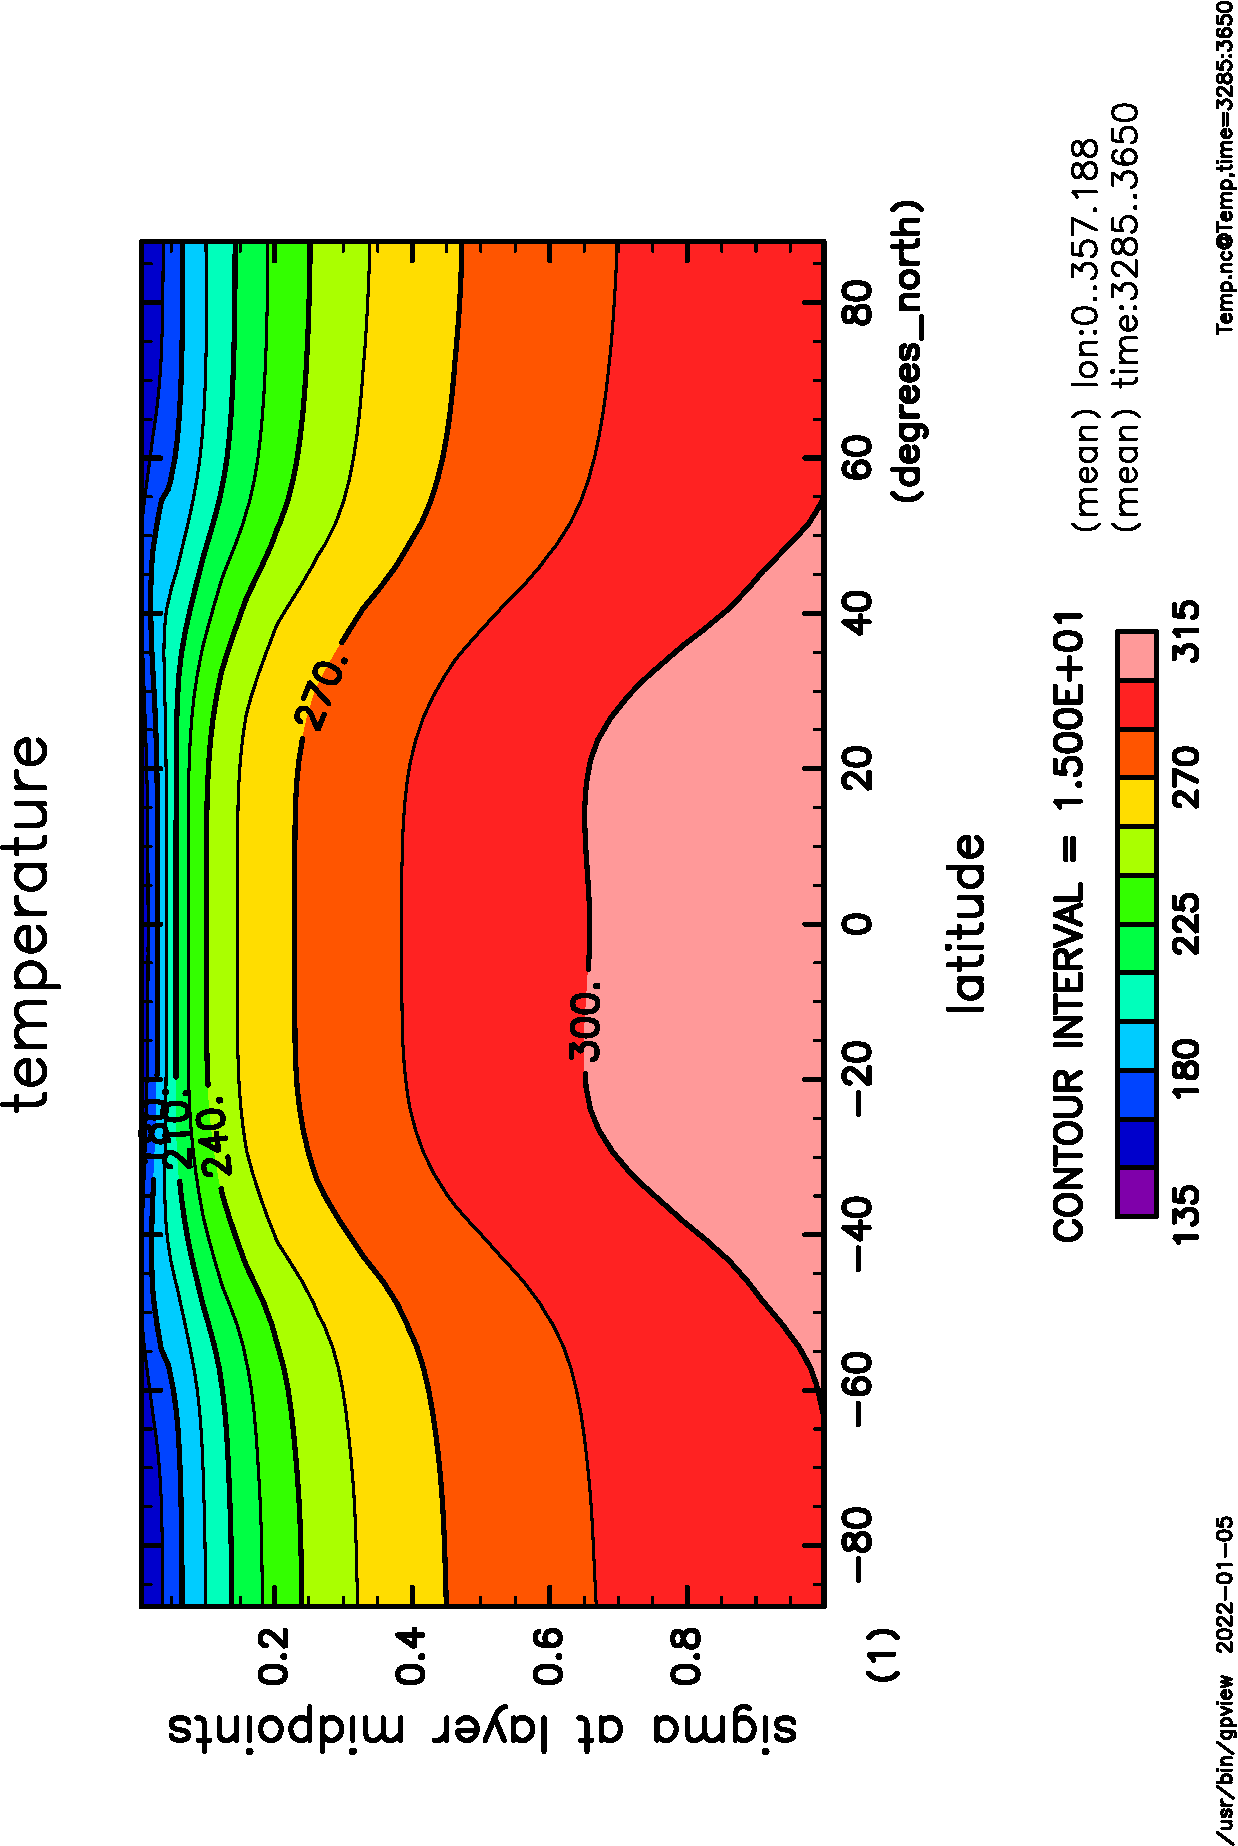
\includegraphics[height=\textwidth,angle=-90]{S1800/Temp,time=3285:3650-crop.pdf}
			\(S=1800\hmu{W/m^2}\)
		\end{column}
		\begin{column}{.3\textwidth}
			\centering
			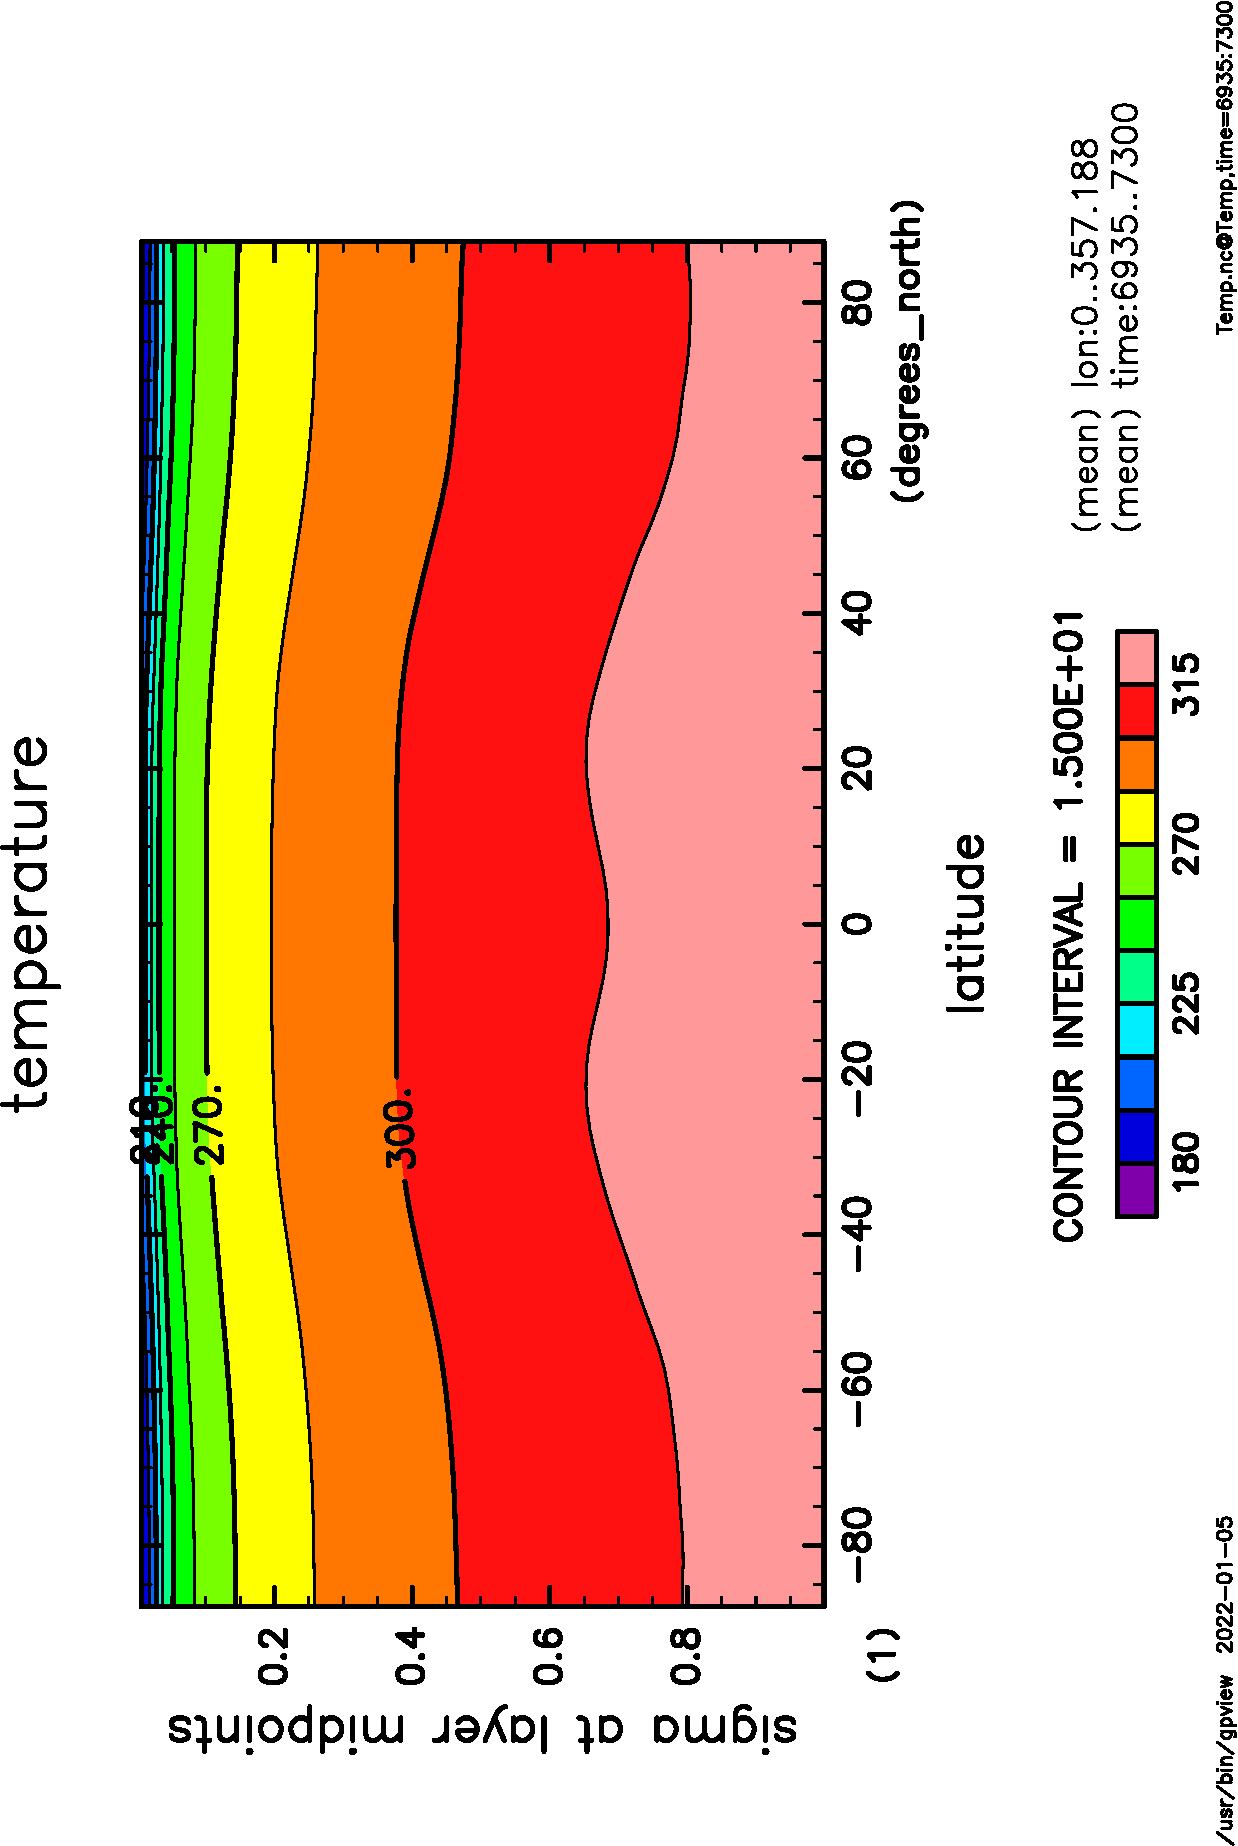
\includegraphics[height=\textwidth,angle=-90]{S2000/Temp,time=6935:7300-crop.pdf}
			\(S=2000\hmu{W/m^2}\)
		\end{column}
	\end{columns}
\end{frame}

\begin{frame}
	\frametitle{結果 (ジオポテンシャル高; 計算終了年での平均)}
	\begin{columns}[T]
		\begin{column}{.3\textwidth}
			\centering
			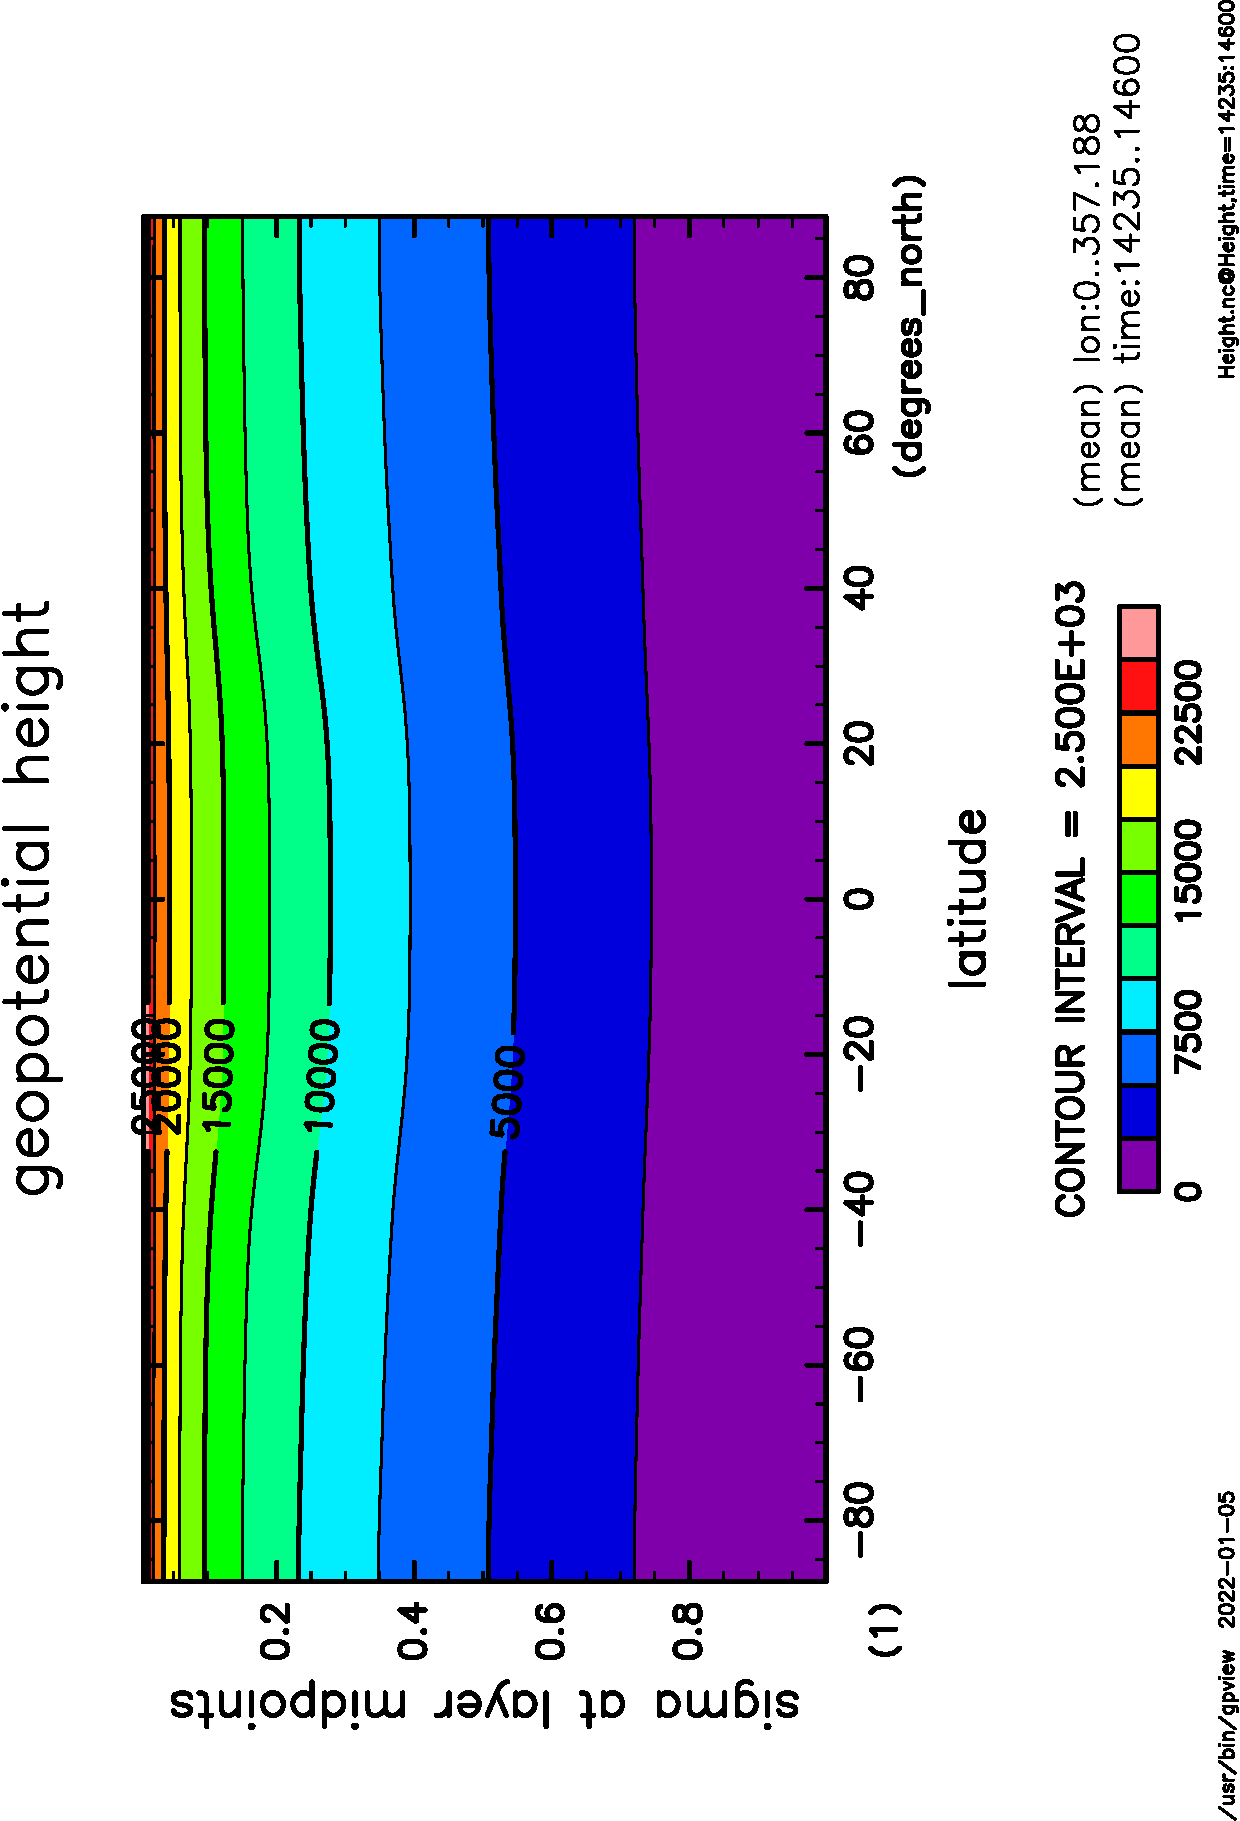
\includegraphics[height=\textwidth,angle=-90]{S1366/Height,time=14235:14600-crop.pdf}
			\(S=1366\hmu{W/m^2}\)\\
			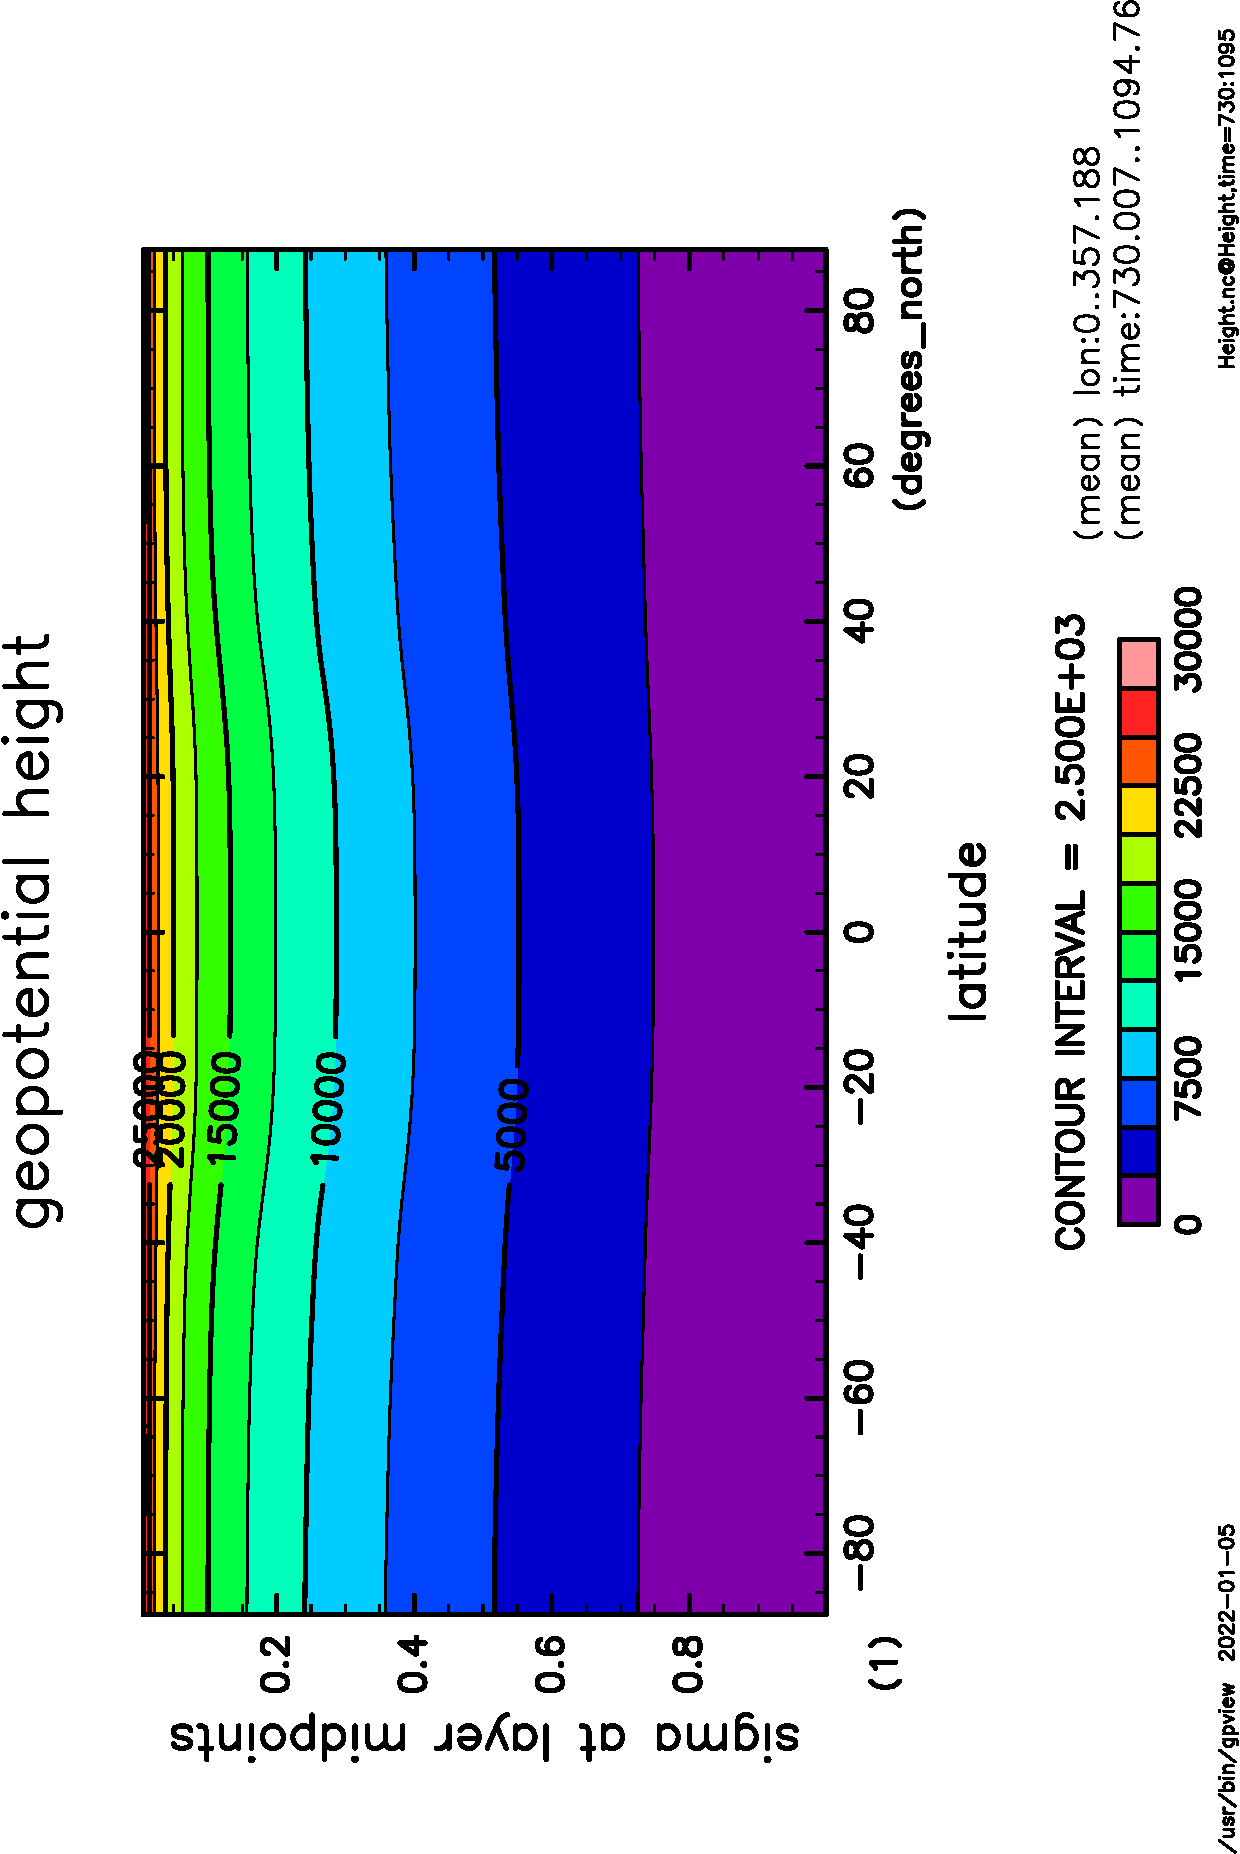
\includegraphics[height=\textwidth,angle=-90]{S1500/Height,time=730:1095-crop.pdf}
			\(S=1500\hmu{W/m^2}\)
		\end{column}
		\begin{column}{.3\textwidth}
			\centering
			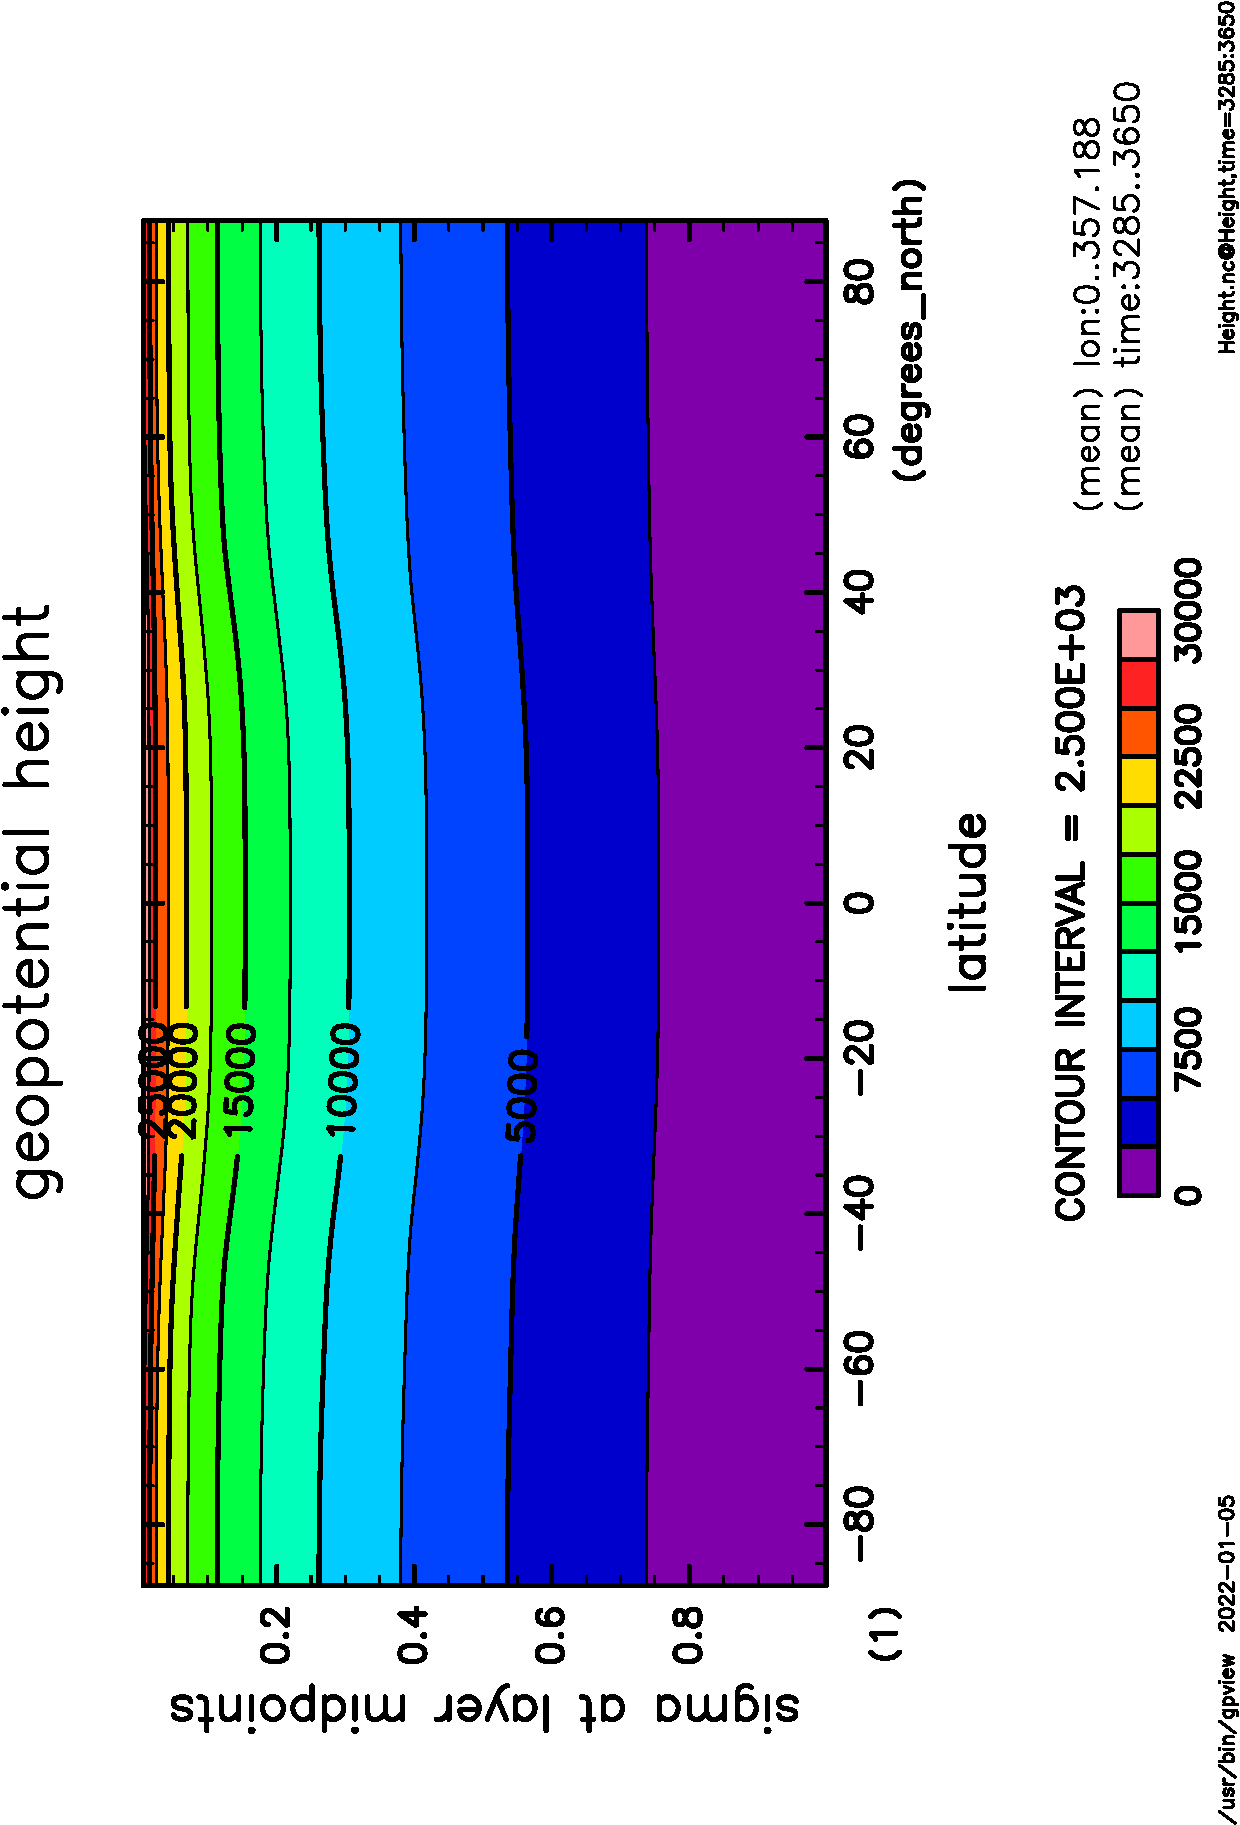
\includegraphics[height=\textwidth,angle=-90]{S1600/Height,time=3285:3650-crop.pdf}
			\(S=1600\hmu{W/m^2}\)\\
			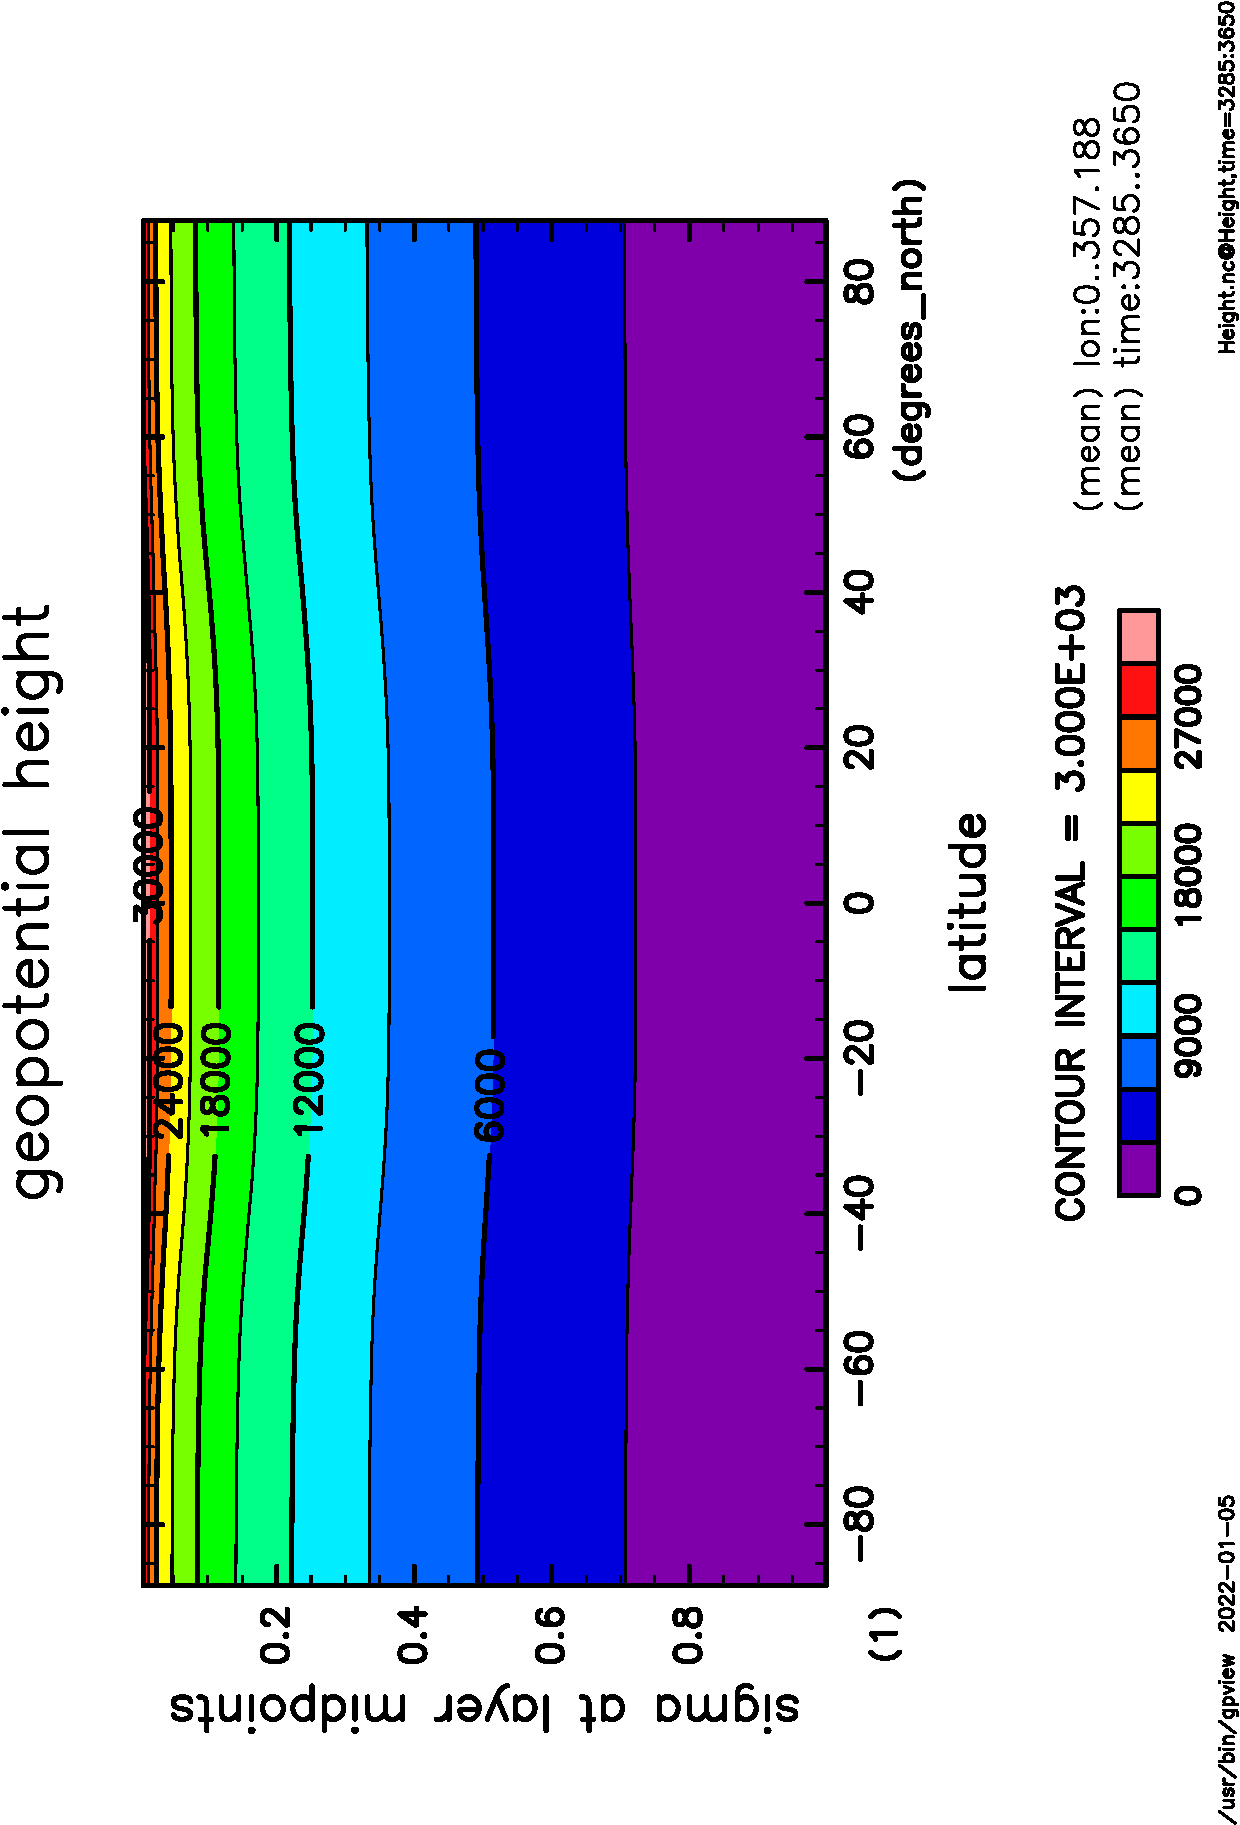
\includegraphics[height=\textwidth,angle=-90]{S1800/Height,time=3285:3650-crop.pdf}
			\(S=1800\hmu{W/m^2}\)
		\end{column}
		\begin{column}{.3\textwidth}
			\centering
			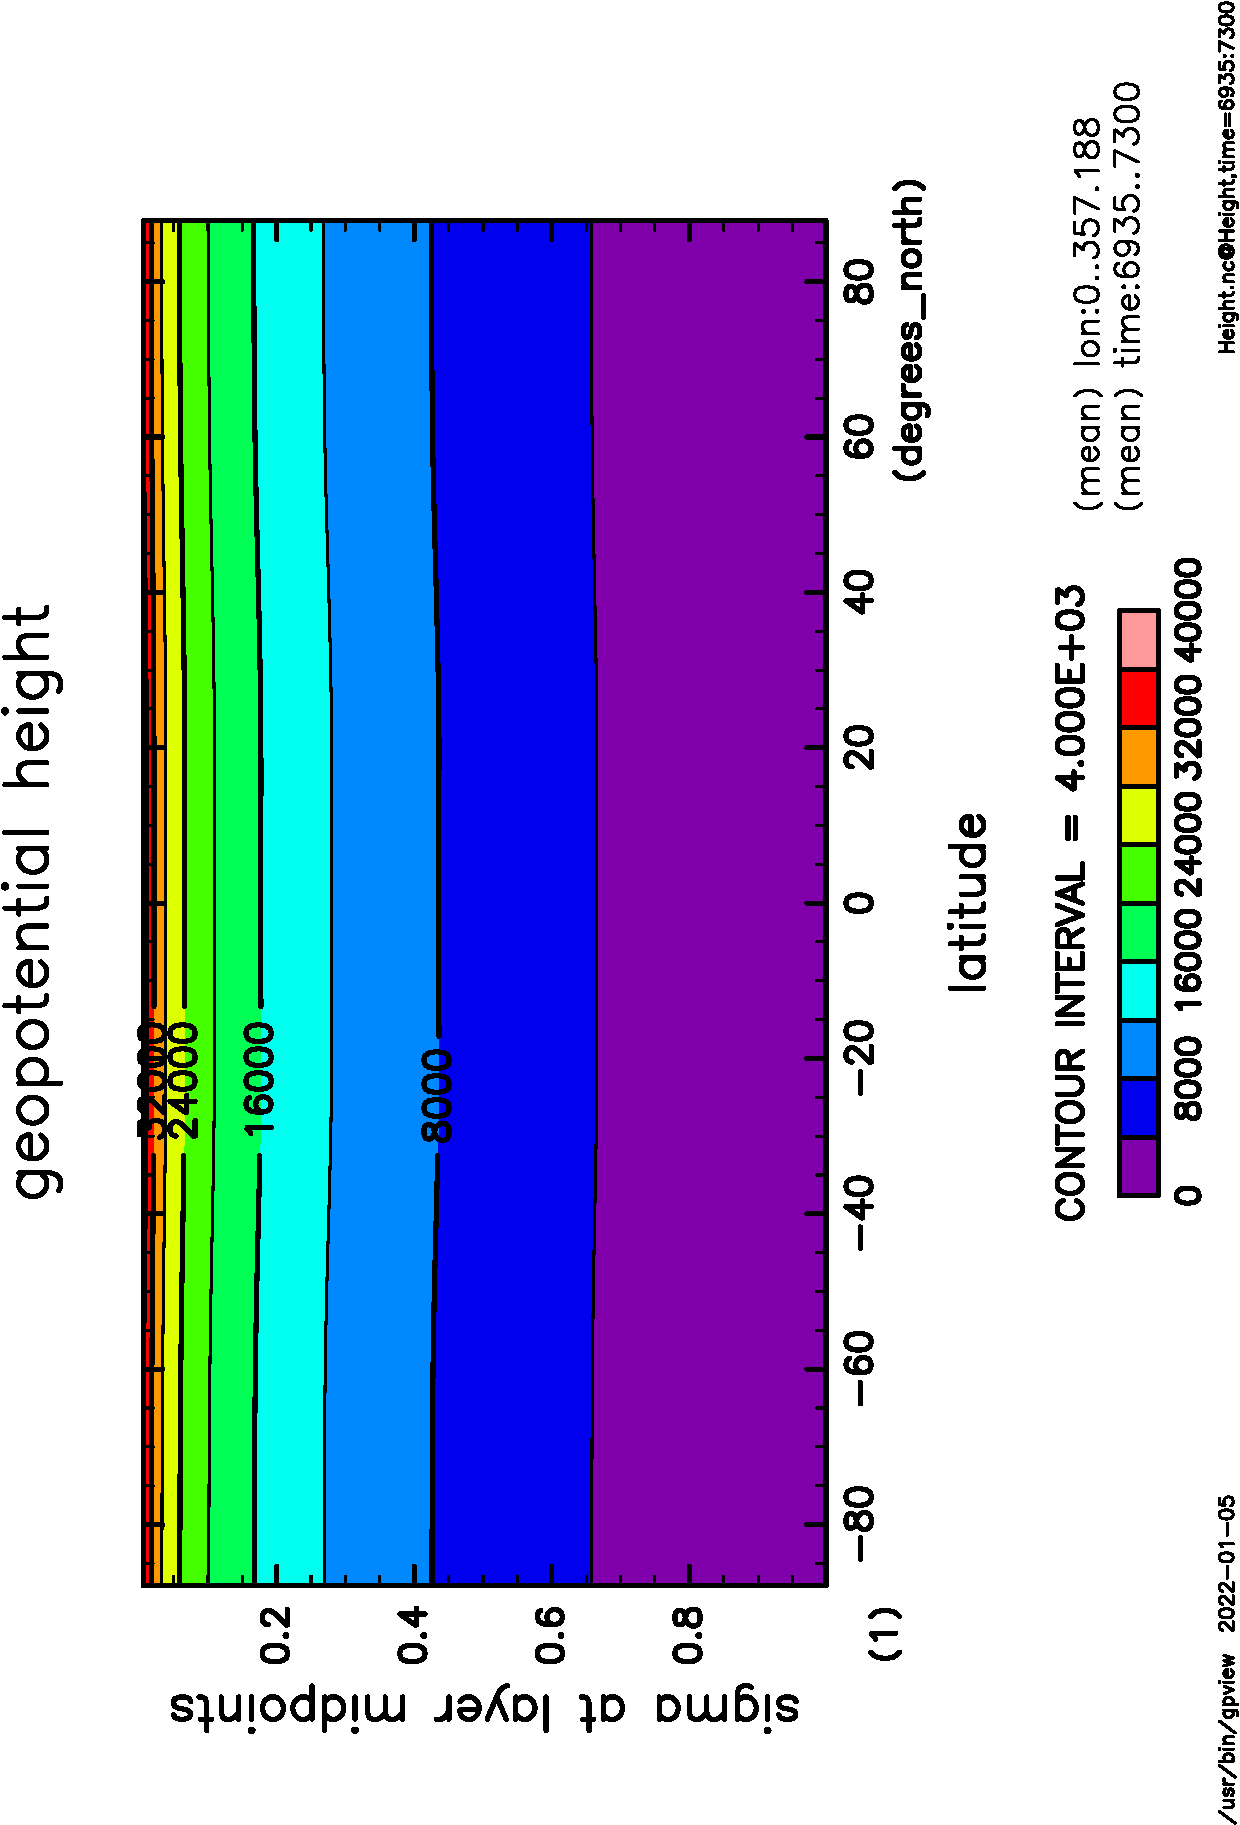
\includegraphics[height=\textwidth,angle=-90]{S2000/Height,time=6935:7300-crop.pdf}
			\(S=2000\hmu{W/m^2}\)
		\end{column}
	\end{columns}
\end{frame}

\begin{frame}
	\frametitle{考察}
	\begin{itemize}
		\item 太陽定数が大きくなると潜熱輸送が大きくなる
		\item 潜熱輸送を大きくしているのは何?(今後の課題)
		\item 地表面温度の差が小さくなるのに、どうして輸送量は増えるのか?
	\end{itemize}
\end{frame}

\end{document}
